\documentclass[brazil,hardcopy,openany]{ufscthesis} %,a5paper
\usepackage[brazil]{babel}
\usepackage{amsfonts, amsmath, amsthm, amsbsy,amssymb,bm,mathtools} % For math fonts, symbols and environments %
\usepackage{graphicx} 		% Required for including images
\usepackage{transparent}	% may be required for inkscape pdf figures (http://bit.ly/18i5Oga)
\usepackage{listings}
\usepackage{caption}
\usepackage{multirow}
\usepackage{lscape}
\usepackage[T1]{fontenc}
\sloppy
\usepackage{siunitx}
\usepackage{nameref}
\usepackage{float}
\usepackage{subfig}

\newcommand{\source}[1]{\small \caption*{Fonte: {#1}} } % Criar fonte embaixo da figura

\newsubfloat{figure}		% Allow subfloats in figure environment (http://bit.ly/1C20NAj)
\graphicspath{{figures/}} 	% Location of the graphics files

\usepackage{siunitx} % units package
\let\DeclareUSUnit\DeclareSIUnit
\let\US\SI
\let\us\si
\DeclareUSUnit\inch{in}
\sisetup{detect-all}  %it may be necessary to load it after loading the font package

%----------------------------------------------------------------------
% Comandos criados pelo usuário
\newcommand{\afazer}[1]{{\color{red}{#1}}} % Para destacar uma parte a ser trabalhada
\DeclareMathOperator*{\argmin}{\arg\!\min}
\DeclareMathOperator*{\argmax}{\arg\!\max}

\newcommand{\sasize}{1}
\newcommand{\annsize}{.7}
\newcommand{\figsize}{.6}
%\newcommand{\figsize}{.7}

%----------------------------------------------------------------------
% Identificadores do trabalho
% Usados para preencher os elementos pré-textuais
\instituicao[a]{Universidade Federal de Santa Catarina} % Opcional
\departamento[a]{Biblioteca Universitária}
\programa[o]{Programa de Pós-Graduação em Engenharia Civil} 
\curso{Engenharia de Engenharia Civil}
\documento[a]{Dissertação} % [o] para dissertação e trabalho de conclusão de curso [a] para tese
\grau{Mestre} % doutor, mestre, engenheiro, etc.
\titulo{PREDIÇÃO DE CONFORTO TÉRMICO EM ESCRITÓRIOS VENTILADOS NATURALMENTE POR MEIO DE REDES NEURAIS ARTIFICIAIS}
\subtitulo{} % Opcional
\autor{Marcelo Salles Olinger}
\local{Florianópolis} % Opcional (Florianópolis é o padrão)
\data{24}{junho}{2019}
\orientador[Universidade Federal de Santa Catarina]{Profa. Ana Paula Melo, Dra.}
\coorientador[Universidade Federal de Santa Catariana]{Prof. Roberto Lamberts, Phd.}
\coordenador[Universidade Federal de Santa Catariana]{Prof. Fulano de Tal, Dr.}
\orientadornabanca{sim} % Se faz parte da banca definir como sim
\coorientadornabanca{sim} % Se faz parte da banca definir como sim
\bancaMembroA{Prof. Saulo Guths, Dr.\\Universidade Federal de Santa Catarina}  %Nome do presidente da banca
\bancaMembroB{Prof. Membro Dois, Dr.\\Universidade Federal de Santa Catarina}   % Nome do membro da Banca
\bancaMembroC{Profa. Membro Três, Dra.\\Outra Universidade} % Nome do membro da Banca
% \bancaMembroD{Quarto membro\\Universidade ...} % Nome do membro da Banca
% \bancaMembroE{Quinto membro\\Universidade ...}  % Nome do membro da Banca
% \bancaMembroF{Sexto membro\\Universidade ...}   % Nome do membro da Banca
% \bancaMembroG{Sétimo membro\\Universidade ...}  % Nome do membro da Banca

%\dedicatoria{Dedico essa conquista aos amigos e familiares que tornaram isso possível.}

%\agradecimento{Inserir os agradecimentos aos colaboradores à execução do trabalho. Inserir os agradecimentos aos colaboradores à execução do trabalho.}

\epigrafe{All models are wrong, but some are useful.}{George E. P. Box}

\textoresumo { % CITAR ESCRITÓRIOS ETC
O condicionamento de ar para resfriamento de edificações é responsável por parcela significativa do consumo energético no mundo, e isso tende a aumentar nas próximas décadas. Uma solução para a mitigação do aumento no consumo de energia para resfriamento de ar é uso de ventilação natural (VN). 
A VN é uma técnica de resfiramento passivo com um potencial significativo de aplicação em países de clima quente. 
Apesar de seu pontencial de aplicabilidade, o uso de VN em edifícios de escritórios
vem diminuindo gradualmente no Brasil, pois edificações de escritórios recentes vêm sendo projetadas exclusivamente com sistemas de condicionamento de ar.

Para que seja aplicada de forma efetiva, é importante que a VN seja concebida desde a fase inicial de projeto. Durante a fase inicial de projeto, há pouco detalhamento relacionado ao projeto arquitetônico, e há necessidade de agilidade nas tomadas de decisão.
Diante deste cenário, uma ferramenta capaz de estimar o conforto térmico em edificações de forma simples e rápida pode ser de grande utilidade.

O objetivo deste estudo é desenvolver um metamodelo de rede neural artificial capaz de estimar o conforto térmico em edificações de escritórios ventilados naturalmente. 
O indicador de conforto térmico utilizado é a fração de horas do ano em que há desconforto térmico por calor no ambiente (EHF), de acordo com o método adaptativo da ASHRAE Standard 55 (2017), para 80\% de aceitabilidade entre os ocupantes.

O metamodelo é desenvolvido a partir de uma base de dados de simulações termoenergéticas obtidas através do programa computacional EnergyPlus. Os modelos que compõem a base de dados foram definidos a partir das características comumente encontradas em edificações de escritórios da cidade de São Paulo. A definição dos parâmetros variados no desenvolvimento dos modelos é estabelecida através da análise de sensibilidade global de Sobol.

O treinamento da rede neural artificial é realizado com uma base de dados de 100.000 simulações termoenergéticas, amostradas pelo método de amostragem do hipercubo latino. 
O desempenho do metamodelo foi avaliado para uma amostra de validação com 20.000 casos, e obteve resultados de EHF com um erro absoluto médio igual a 0,009, e um erro absoluto do 95º percentil igual a 0,024.

O metamodelo desenvolvido foi capaz de estimar o conforto térmico em edificações de escritórios ventilados naturalmente para a cidade de São Paulo com resultados próximos aos obtidos pelo programa de simulação computacional EnergyPlus.
Esse metamodelo pode ser utilizado por projetistas como uma ferramenta de fácil aplicação no suporte à tomada de decisão em fases iniciais de projeto.
}
\palavraschave{Ventilação natural. Metamodelo. Simulação termoenergética de edificações.}

\textabstract {
	Energy demand in the world for air cooling in buildings is significant, and it is expected to increase in the next decades.
	Natural ventilation (NV) could be a solution to mitigate energy use for air cooling, since it is a passive cooling strategy with significant potential for hot climates.
	Despite its potential, the use of NV has been decreasing in recent years for office buildings in Brazil, since the design of buildings with air conditioning prevails.
	
	It is important to conceive the use of NV since early-design phases of the building to guarantee its effectiveness.
	During early-design phases, there are uncertainties related to the many construction parameters, and the decision process has to occur fast.
	Given the current scenario, the development of a surrogate model capable of estimate thermal comfort in buildings in a simple and fast way could be of great use.
	
	The aim of this study is to develop an artificial neural network model to estimate thermal comfort in naturally ventilated office buildings.
	The annual fraction of occupied hours within the thermal zone with operative temperatures above the upper limit of ASHRAE's Standards 55 (2017) adaptive model, for 80\% of acceptability, is used as a thermal comfort index.
	
	The surrogate model is developed from a data set of building performance simulations, using the software EnergyPlus.
	Simulation models were defined based on a database of naturally ventilated office buildings in the city of São Paulo.
	The variables used as inputs in the surrogate model are defined by Sobol's sensitivity analysis.
	
	From data of 100,000 simulations, sampled by Latin hypercube sampling method, the neural network was trained.
	The performance of the surrogate model was measured with a validation data set of 20,000 cases.
	The mean absolute error for the fraction of hours outside ASHRAE's Standards 55 (2017) adaptive model limits for the validation data set was 0,009, and the absolute error of the 95$^{th}$ percentile was 0,024.
	
	The final surrogate model achieved estimates for thermal comfort in naturally ventilated office buildings in the city of São Paulo with results close to the simulations developed on the software EnergyPlus. This surrogate model can be used by building designers as a simple tool to support decision making in early-design phases.
}
\keywords{Natural ventilation. Surrogate model. Building performance simulation.}

%\gls{q} \Gls{latex} \Glspl{formula} \acrshort{gcd} \acrlong{DCC} \acrfull{lcm}
% Abreviaturas
\newacronym{vn}{VN}{ventilação natural}
\newacronym{iea}{IEA}{Agência Internacional de Energia}
\newacronym{aivc}{AIVC}{\textit{Air Infiltration and Ventilation Centre}}
\newacronym{hvac}{HVAC}{\textit{heating, ventilating and air conditioning}}
\newacronym{pmv}{PMV}{voto predito médio}
\newacronym{ann}{ANN}{redes neurais artificiais}
\newacronym{svm}{MVS}{máquinas de vetores de suporte}
\newacronym{cfd}{CFD}{\textit{Computer Fluid Dynamics}}
\newacronym{afn}{AFN}{\textit{Airflow Network}}
\newacronym{ct}{CT}{capacidade térmica}
\newacronym{cp}{$C_p$}{coeficientes de pressão do vento}
\newacronym{cq}{$C_Q$}{coeficiente de fluxo mássico de ar}
\newacronym{cpeq}{$C_{p,eq}$}{coeficiente de pressão equivalente}
\newacronym{cd}{$C_d$}{coeficiente de descarga}
\newacronym{tpu}{TPU}{Universidade Politécnica de Tóquio}
\newacronym{paf}{PAF}{percentual de abertura na fachada}
\newacronym{fs}{FS}{fator solar}
\newacronym{as}{AS}{análise de sensibilidade}
\newacronym{ehf}{EHF}{fração de horas de desconforto por calor}
\newacronym{ach}{ACH}{trocas de ar por hora}
\newacronym{rmse}{RMSE}{raiz quadrada do erro quadrático médio}
\newacronym{nrmse}{NRMSE}{raiz quadrada do erro quadrático médio normalizada}
\newacronym{r2}{R$^2$}{coeficiente de determinação}
\newacronym{abse}{MAE}{erro absoluto médio}
\newacronym{ae95}{AE95}{erro absoluto do 95º percentil}
\newacronym{ma}{MA}{método analítico}
\newacronym{inic}{INI-C}{Proposta de Instrução Normativa do Inmetro para a Classe de Eficiência Energética de Edificações Comerciais, de Serviços e Públicas}
 

%List of Symbols
\newglossaryentry{px}{	% how the symbol will be called in the text \gls{x}
	type=symbols,		% set the glossary entry type as "symbol"
	name={\ensuremath{P_x}},	
	description={pressão estática do ar em um ponto da fachada do edifício},
	user1=\unexpanded{\si{\pascal}}
}
\newglossaryentry{p0}{	% how the symbol will be called in the text \gls{x}
type=symbols,		% set the glossary entry type as "symbol"
name={\ensuremath{P_0}},	
description={pressão estática de referência do ar},
user1=\unexpanded{\si{\pascal}}
}
\newglossaryentry{pd}{	% how the symbol will be called in the text \gls{x}
type=symbols,		% set the glossary entry type as "symbol"
name={\ensuremath{P_d}},	
description={pressão dinâmica do ar},
user1=\unexpanded{\si{\pascal}}
}
\newglossaryentry{rho}{	% how the symbol will be called in the text \gls{x}
type=symbols,		% set the glossary entry type as "symbol"
name={\ensuremath{\rho}},	
description={densidade do ar},
user1=\unexpanded{\si{\kilogram/\cubic\meter}}
}
\newglossaryentry{vref}{	% how the symbol will be called in the text \gls{x}
type=symbols,		% set the glossary entry type as "symbol"
name={\ensuremath{V_{ref}}},	
description={velocidade de referência do vento},
user1=\unexpanded{\si{\meter/\second}}
}
\newglossaryentry{tinf}{	% how the symbol will be called in the text \gls{x}
type=symbols,		% set the glossary entry type as "symbol"
name={\ensuremath{T_{inf}}},	
description={limite inferior da temperatura operativa para 80\% de aceitabilidade no conforto térmico},
user1=\unexpanded{\si{\celsius}}
}
\newglossaryentry{tsup}{	% how the symbol will be called in the text \gls{x}
type=symbols,		% set the glossary entry type as "symbol"
name={\ensuremath{T_{sup}}},	
description={limite superior da temperatura operativa para 80\% de aceitabilidade no conforto térmico},
user1=\unexpanded{\si{\celsius}}
}
\newglossaryentry{tm}{	% how the symbol will be called in the text \gls{x}
type=symbols,		% set the glossary entry type as "symbol"
name={\ensuremath{T_m}},	
description={temperatura média do ar externo},
user1=\unexpanded{\si{\celsius}}
}
\newglossaryentry{tssup}{	% how the symbol will be called in the text \gls{x}
type=symbols,		% set the glossary entry type as "symbol"
name={\ensuremath{timesteps_{sup}}},	
description={número de \textit{timesteps} em que há ocupação na zona térmica e a temperatura operativa ultrapassa o limite superior determinado pelo método adaptativo}%,
%user1= {-} %\unexpanded{\si{\celsius}}
}
\newglossaryentry{tsocup}{	% how the symbol will be called in the text \gls{x}
type=symbols,		% set the glossary entry type as "symbol"
name={\ensuremath{timesteps_{sup}}},	
description={número de \textit{timesteps} em que há ocupação na zona térmica}%,
%user1= {-} %\unexpanded{\si{\celsius}}
}

\newglossaryentry{tsupv}{	% how the symbol will be called in the text \gls{x}
	type=symbols,		% set the glossary entry type as "symbol"
	name={\ensuremath{T_{sup,v}}},	
	description={temperatura limite superior na faixa de conforto, considerando-se a velocidade do ar},
	user1= \unexpanded{\si{\celsius}}
}
\newglossaryentry{tvar}{	% how the symbol will be called in the text \gls{x}
type=symbols,		% set the glossary entry type as "symbol"
name={\ensuremath{T_{v_{ar}}}},	
description={margem extra de temperatura permitida pela consideração da velocidade do ar},
user1= \unexpanded{\si{\celsius}}
}
\newglossaryentry{deltacp}{	% how the symbol will be called in the text \gls{x}
type=symbols,		% set the glossary entry type as "symbol"
name={\ensuremath{\overline{\Delta}_{Cp}}},
description={diferença absoluta média entre os valores dos Cp's obtidos pela base da TPU e obtidos pelo MA},
user1= {-}%\unexpanded{\si{\celsius}}
}
\newglossaryentry{alphaj}{	% how the symbol will be called in the text \gls{x}
type=symbols,		% set the glossary entry type as "symbol"
name={\ensuremath{\alpha_j}},	
description={ângulo de incidência do vento  sobre a fachada, e tem valor igual a $30 \cdot j$},
user1= \ensuremath{^{\circ}}
}
\newglossaryentry{meancptpu}{	% how the symbol will be called in the text \gls{x}
type=symbols,		% set the glossary entry type as "symbol"
name={\ensuremath{\overline{Cp}^{TPU}_{f_i,\alpha_j}}},	
description={valor médio dos Cp's disponibilizados pela base de dados da TPU para a fachada $i$ de uma edificação, para o ângulo de incidência do vento igual a $\alpha_j$}, %\glsname{tpu} \glsname{alphaj}}
user1= {-}%\unexpanded{\si{\celsius}}
}
\newglossaryentry{cpma}{	% how the symbol will be called in the text \gls{x}
type=symbols,		% set the glossary entry type as "symbol"
name={\ensuremath{Cp^{MA}_{f_i,\alpha_j}}},	
description={Cp calculado pelo MA para a fachada de uma edificação com proporções iguais às da fachada $i$, para o ângulo de incidência do vento igual a $\alpha_j$}, %\glsname{ma} \glsname{alphaj}
user1= {-}%\unexpanded{\si{\celsius}}
}
\newglossaryentry{fi}{	% how the symbol will be called in the text \gls{x}
type=symbols,		% set the glossary entry type as "symbol"
name={\ensuremath{f_i}},	
description={fachada $i$ da edificação avaliada},
user1= {-}%\unexpanded{\si{\celsius}}
}
\newglossaryentry{m}{	% how the symbol will be called in the text \gls{x}
type=symbols,		% set the glossary entry type as "symbol"
name={\ensuremath{\dot{m}_{i,j}}},	
description={fluxo de ar entre os pontos $i$ e $j$, quando a porta/janela está aberta},
user1=\unexpanded{\si{\kilogram/\second}}
}
\newglossaryentry{n}{	% how the symbol will be called in the text \gls{x}
type=symbols,		% set the glossary entry type as "symbol"
name={\ensuremath{\dot{n}_{i,j}}},	
description={fluxo de ar entre os pontos $i$ e $j$, quando a porta/janela está fechada},
user1=\unexpanded{\si{\kilogram/\second}}
}
\newglossaryentry{theta}{	% how the symbol will be called in the text \gls{x}
	type=symbols,		% set the glossary entry type as "symbol"
	name={\ensuremath{\Theta}},	
	description={fração de abertura da porta/janela},
	user1={-} %\unexpanded{\si{\kilogram/\second}}
}
\newglossaryentry{height}{	% how the symbol will be called in the text \gls{x}
type=symbols,		% set the glossary entry type as "symbol"
name={\ensuremath{H}},	
description={altura da abertura},
user1= \unexpanded{\si{\meter}}
}
\newglossaryentry{width}{	% how the symbol will be called in the text \gls{x}
type=symbols,		% set the glossary entry type as "symbol"
name={\ensuremath{W}},	
description={largura da abertura},
user1= \unexpanded{\si{\meter}}
}
\newglossaryentry{piz}{	% how the symbol will be called in the text \gls{x}
type=symbols,		% set the glossary entry type as "symbol"
name={\ensuremath{P_{i(z)}}},	
description={pressão de ar no ponto $i$, altura $z$},
user1= \unexpanded{\si{\pascal}}
}
\newglossaryentry{cqq}{	% how the symbol will be called in the text \gls{x}
type=symbols,		% set the glossary entry type as "symbol"
name={\ensuremath{C_Q}},	
description={coeficiente de fluxo mássico de ar da abertura},
user1={-} %\unexpanded{\si{\kilogram/\second}}
}
\newglossaryentry{cdd}{	% how the symbol will be called in the text \gls{x}
type=symbols,		% set the glossary entry type as "symbol"
name={\ensuremath{C_d}},	
description={coeficiente de descarga da abertura},
user1={-} %\unexpanded{\si{\kilogram/\second}}
}
\newglossaryentry{cpp}{	% how the symbol will be called in the text \gls{x}
type=symbols,		% set the glossary entry type as "symbol"
name={\ensuremath{C_p}},	
description={coeficiente de pressão},
user1={-} %\unexpanded{\si{\kilogram/\second}}
}
\newglossaryentry{cppeq}{	% how the symbol will be called in the text \gls{x}
type=symbols,		% set the glossary entry type as "symbol"
name={\ensuremath{C{_p,eq}}},	
description={coeficiente de pressão equivalente},
user1={-} %\unexpanded{\si{\kilogram/\second}}
}
\newglossaryentry{exp}{	% how the symbol will be called in the text \gls{x}
type=symbols,		% set the glossary entry type as "symbol"
name={\ensuremath{exp}},	
description={ expoente de fluxo de massa de ar},
user1={-} %\unexpanded{\si{\kilogram/\second}}
}
\newglossaryentry{pzn}{	% how the symbol will be called in the text \gls{x}
type=symbols,		% set the glossary entry type as "symbol"
name={\ensuremath{P_{zn}}},	
description={pressão do ar na zona térmica analisada},
user1=\unexpanded{\si{\pascal}}
}
\newglossaryentry{pi}{	% how the symbol will be called in the text \gls{x}
type=symbols,		% set the glossary entry type as "symbol"
name={\ensuremath{P_i}},	
description={pressão do ar na zona térmica, ligada pela porta $i$},
user1=\unexpanded{\si{\pascal}}
}
\newglossaryentry{np}{	% how the symbol will be called in the text \gls{x}
type=symbols,		% set the glossary entry type as "symbol"
name={\ensuremath{N_P}},	
description={número de portas que se conectam à zona térmica}
}
\newglossaryentry{nj}{	% how the symbol will be called in the text \gls{x}
type=symbols,		% set the glossary entry type as "symbol"
name={\ensuremath{N_J}},	
description={número de janelas que se conectam à zona térmica}
}
\newglossaryentry{li}{	% how the symbol will be called in the text \gls{x}
type=symbols,		% set the glossary entry type as "symbol"
name={\ensuremath{L_i}},	
description={perímetro da porta $i$},
user1= \unexpanded{\si{\meter}}
}
\newglossaryentry{area}{	% how the symbol will be called in the text \gls{x}
type=symbols,		% set the glossary entry type as "symbol"
name={\ensuremath{A_j}},	
description={área da janela $j$},
user1= \unexpanded{\si{\square\meter}}
}
\newglossaryentry{pext}{	% how the symbol will be called in the text \gls{x}
type=symbols,		% set the glossary entry type as "symbol"
name={\ensuremath{P_{ext}}},	
description={pressão do ar no ambiente externo},
user1=\unexpanded{\si{\pascal}}
}
\newglossaryentry{cpj}{	% how the symbol will be called in the text \gls{x}
type=symbols,		% set the glossary entry type as "symbol"
name={\ensuremath{C_{p,j}}},	
description={Cp na superície da janela $j$},
user1={-} %\unexpanded{\si{\kilogram/\second}}
}
\newglossaryentry{deltamet}{	% how the symbol will be called in the text \gls{x}
type=symbols,		% set the glossary entry type as "symbol"
name={\ensuremath{\delta_{met}}},	
description={espessura da camada limite para o perfil de vento na estação meteorológica},
user1=\unexpanded{\si{\meter}}
}
\newglossaryentry{alphamet}{	% how the symbol will be called in the text \gls{x}
type=symbols,		% set the glossary entry type as "symbol"
name={\ensuremath{\alpha_{met}}},	
description={expoente para o perfil de vento na estação meteorológica},
user1={-} %\unexpanded{\si{\kilogram/\second}}
} % para atualizar a lista, usar o comando "makeglossaries dissertacao" no terminal
\begin{document}

	
	%--------------------------------------------------------
	\frontmatter
	% Elementos pré-textuais
	\folhaderosto[] %[pre/Ficha_Catalografica.pdf]
%	\folhadeaprovacao{}{} %{pre/signature_page_color.pdf}{}
	%\paginadedicatoria
	%\paginaagradecimento
	\paginaepigrafe
	\paginaresumo
	\paginaabstract
	% ---
	\listadefiguras % as listas dependem da necessidade do usuário
	\listadetabelas 
	%\gls{q} \Gls{latex} \Glspl{formula} \acrshort{gcd} \acrlong{DCC} \acrfull{lcm}
	\listadeabreviaturas
	\listadesimbolos
	\sumario
	%--------------------------------------------------------
	\mainmatter

\chapter{Introdução}
\label{chapter:introducao}

De acordo com a \acrlong{iea} \cite{IEA2018a}, no ano de 2017 o setor de edificações representou mais de 30\% do consumo final total de energia no mundo. 
O relatória da \citeonline{IEA2018} aponta que a demanda por energia destinada ao resfriamento de ar em edificações mais que triplicou do ano de 1990 a 2016 e, se não houver mudanças no cenário atual, estima-se que essa demanda mais que triplicará até o ano de 2050, representando 37\% do aumento no consumo de eletricidade em edificações. Isso corresponderá a 11,5\% do consumo de energia total em edificações comerciais. 
O potencial de aumento na demanda por energia destinada ao resfriamento de ar em países de clima quente é ainda mais expressivo. Das 2,8 bilhões de pessoas que vivem nas partes mais quentes do mundo hoje, apenas 8\% possuem sistema de condicionamento de ar \cite{IEA2018}. No Brasil, a parcela do resfriamento de ar nas cargas de pico das redes elétricas em 2016 correspondia a 7,6\% do total, e a estimativa, considerando-se o cenário base, é de que essa parcela represente 30,8\% da carga de pico até o ano de 2050 \cite{IEA2018}. 
%No Brasil, desde 2009 o INMETRO possui um programa de etiquetagem de edificações voltado para padrões de eficiência energética de edificações \cite{BRASIL2009}.

Esse contexto evidencia a necessidade de medidas mitigadoras relacionadas ao consumo energético destinado ao resfriamento de edificações. O uso de técnicas de resfriamento passivo, como a \acrfull{vn}, pode ser uma solução. O resfriamento passivo é um conjunto de técnicas sustentáveis para resfriar edifícios por meios naturais \cite{Samani2016}, que consiste em qualquer sistema que busca minimizar, ou eliminar, se possível, o uso de sistemas de condicionamento de ar, com o objetivo de reduzir as altas temperaturas internas e o consumo de energia para resfriamento, proporcionando conforto térmico aos ocupantes.

Técnicas de \acrshort{vn} são encontradas ao longo de toda a história na arquitetura vernacular \cite{Pesic2018}, e hoje vêm sendo atualizadas de acordo com novos estudos no campo de conforto térmico e projetos sustentáveis de edificações.
Além de assegurar a qualidade do ar, a \acrshort{vn} promove o resfriamento da edificação, proporcionando conforto térmico aos usuários quando as condições do clima externo são favoráveis \cite{Yao2009}.

Apesar de um quinto da energia elétrica brasileira ser destinada a edificações comerciais, de serviços e públicas \cite{EPE2018}, o uso de \acrshort{vn} em edifícios de escritórios vem diminuindo gradualmente no Brasil. De acordo com \citeonline{Alves2017}, apesar do uso de sistemas de condicionamento de ar e iluminação mais eficientes, edifícios da cidade de Belo Horizonte construídos a partir dos anos 2000 tendem a ser os maiores consumidores de energia, por não adotarem estratégias de resfriamento passivo.

Para que o conforto térmico dos usuários seja garantido sem um consumo significativo de energia, é importante entender como ocorrem as variações térmicas em um edifício antes de construí-lo. Análises durante os estágios iniciais de projeto de uma edificação com \acrshort{vn} apontam decisões fundamentais para o desempenho térmico. No estágio inicial de projeto, o potencial de otimização é significativo, e nesta etapa qualquer estimativa do conforto e desempenho energético da edificação pode refletir nas tomadas de decisão \cite{Belleri2014, Roetzel2014}.

O método mais avançado de se estimar o desempenho termoenergético de edificações atualmente é por meio de simulações computacionais. No entanto, esse processo exige o conhecimento técnico de um especialista, pois simulações termoenergéticas dinâmicas requerem modelos detalhados e enfrentam diversos problemas, associados principalmente a informações necessárias para dados de entrada do modelo processado \cite{Corgnati2013}. No contexto brasileiro, a análise do desempenho térmico de edificações por meio de simulações computacionais é uma medida relevante, pois, assim como em outros países em desenvolvimento, a falta de acessibilidade a dados relacionados a padrões de consumo de energia e atributos físicos e operacionais de edifícios de escritório dificulta as análises a partir de bancos de dados \cite{Alves2018}. Uma alternativa para contornar essas questões é o desenvolvimento de modelos a partir de simulações computacionais, os metamodelos. Por meio de metamodelos é possível se obter resultados próximos aos de simulações complexas de desempenho energético.

Metamodelos para eficiência energética de edificações podem ser desenvolvidos a partir de diferentes métodos \cite{Ostergard2018}. A solução mais apropriada depende do contexto e propósitos de cada aplicação.
\citeonline{Versage2015} foi capaz de estimar as cargas térmicas de edificações comerciais através de diferentes métodos de metamodelagem.
\citeonline{Melo2016} desenvolveram um modelo de \acrfull{ann} para estimar graus hora de resfriamento e cargas térmicas de aquecimento e resfriamento em edificações residenciais.
O desenvolvimento de um metamodelo de máquina de vetores de suporte capaz de estimar conforto térmico em edificações comerciais foi proposto por \citeonline{Rackes2016}. Voltado principalmente a tipologias de escolas, o metamodelo estima a fração de horas em desconforto por calor dos ocupantes ao longo do ano.
%
%A \acrshort{vn} em edificações apresenta comportamentos complexos e a avaliação do seu potencial de resfriamento faz-se necessária desde a fase inicial de projeto. Possibilitar esse tipo de análise de forma simples e rápida é fundamental nas tomadas de decisão em projetos de edificações e na aplicação de políticas públicas voltadas à eficiência energética. Por meio de ferramentas de aprendizagem automática, surge a oportunidade de se desenvolver metamodelos capazes de obter resultados de conforto térmico em edificações.

O consumo de energia para resfriamento de edificações é expressivo no mundo, e a expectativa é de que a demanda por energia continue crescendo nas próximas décadas, principalmente em países de climas quentes.
Neste contexto, o uso de técnicas de \acrfull{vn} apresenta-se como uma solução para mitigar o uso de condicionamento de ar.
Entretanto, o desempenho térmico das edificações apresenta fenômenos termofísicos complexos, fazendo com que estimativas de conforto térmico devam ser consideradas preferencialmente desde as etapas iniciais de projeto. 	
Na busca por uma ferramenta capaz de auxiliar projetistas de maneira rápida e simples, surge a possibilidade de utilizar-se metamodelos.
Portanto, este trabalho apresenta o desenvolvimento de um metamodelo capaz de estimar o conforto térmico em edifícios de escritórios ventilados naturalmente.

\section{Objetivos}
\subsection{Objetivo geral}

O objetivo deste estudo é desenvolver um metamodelo capaz de estimar o conforto térmico em edifícios de escritórios ventilados naturalmente.

\subsection{Objetivos específicos}

Dentre os objetivos específicos deste trabalho, destacam-se:

\begin{itemize}
	\item Identificar as características construtivas encontradas em edifícios de escritórios ventilados naturalmente na cidade de São Paulo;
	\item Desenvolver um modelo de simulação termoenergética simplificado, com apenas uma zona térmica, capaz de representar as trocas térmicas de uma sala em um edifício de escritórios;
	\item Definir as variáveis com maior e menor influência no desempenho térmico dos edifícios ventilados naturalmente.
\end{itemize}

\chapter{Revisão de literatura}

\section{Ventilação natural}

A \acrfull{vn} ocorre quando diferenças de pressão geradas pelo vento ou por forças de empuxo agem em uma ou mais aberturas da envoltória de uma edificação \cite{CarrilhodaGraca2016}. Um sistema de \acrshort{vn} pode ser caracterizado pela estratégia de ventilação, locação das aberturas e suas áreas.  \citeonline{CarrilhodaGraca2016} comentam que, apesar de muitos regulamentos exigirem uma área mínima de ventilação, tipicamente definida em função da área de piso, essas exigências se baseiam em grandes simplificações. A área de abertura ideal depende da estratégia de ventilação (unilateral ou cruzada), do clima e dos objetivos relacionados ao período de uso da \acrshort{vn}.

A \acrshort{vn} pode ser aplicada por meio de grelhas, sistemas de dutos, ou simplesmente grandes aberturas, como janelas ou portas. No caso de grandes aberturas, duas configurações podem ser consideradas: ventilação cruzada, ou ventilação unilateral. Na estratégia ventilação unilateral, a turbulência do vento e as variações nos gradientes de pressão induzidos por rajadas podem afetar fortemente o fluxo de ar nas aberturas.
Como esses parâmetros não são estáveis, é mais complicado avaliar a ventilação unilateral em relação à ventilação cruzada \cite{Freire2013}.
\citeonline{CarrilhodaGraca2016} apontam que para otimização da \acrshort{vn} unilateral em edificações pequenas ou médias, para a mesma área total de abertura, duas ou mais aberturas são mais eficientes do que apenas uma, sendo que aberturas espaçadas funcionam melhor do que próximas.	% Ver Stabat, P., Caciolo, M., & Marchio, D. (2012). Progress on single-sided ventilation techniques for buildings. Advances in Building Energy Research, 6(2), 212–241. https://doi.org/10.1080/17512549.2012.740903
Além das diferentes estratégias relacionadas à configuração das aberturas na edificação, há também diferentes abordagens quanto aos períodos de funcionamento. Algumas edificações podem permitir o uso da \acrshort{vn} durante o dia, enquanto outras também permitem o uso de \acrshort{vn} noturna. Há também casos em que a \acrshort{vn} é exclusivamente noturna, e durante o dia utiliza-se sistemas de condicionamento de ar \cite{Pesic2018}.

O mecanismo de \acrlong{vn} noturna é baseado na transferência de calor por convecção da estrutura exposta do edifício para o fluxo de ar frio da noite (momento em que a diferença entre a temperatura do ar interno e externo é maior) \cite{Breesch2010}. Durante o dia, a massa térmica da	edificação é utilizada para acumular os ganhos de calor internos e do sol, e prevenir condições desconfortáveis durante as horas de operação da edificação.	
Isso leva a três consequências: para garantir o funcionamento, o calor deve ser armazenado na estrutura da edificação, e é necessário garantir uma ponte para que haja a transferência de calor para/da estrutura; a ventilação noturna é mais apropriada para climas moderados e frios, com maiores diferenças diárias de temperatura ao longo do dia; como essa tecnologia utiliza apenas calor sensível, é menos aplicável em climas quentes e úmidos.

Prover, efetivamente, \acrshort{vn} em edifícios pode economizar energia e custo em comparação à ventilação mecânica, devido à baixa manutenção e custo zero de operação \cite{Omrani2017}. O desempenho da \acrshort{vn} é medido, primariamente, através de parâmetros de dinâmica dos fluidos, como padrão do fluxo de ar, velocidade média, vazão de ar, distribuição de pressão, renovações de ar, fluxo volumétrico e outras qualidades que podem ser derivadas desses parâmetros.
Esses elementos do fluxo também podem ser usados para determinar características mais amplas do ambiente interno de edificações, como a qualidade do ar e o conforto térmico. Há diferentes métodos de avaliação de desempenho de \acrshort{vn}, cada um com suas vantagens e limitações. O método escolhido deve ser o mais apropriado, baseado nos recursos, exigências e estágio do projeto.

Estimar o desempenho da \acrshort{vn} no projeto da edificação envolve a consideração de fenômenos físicos complexos, o que pode ser dificultoso. Para a simulação computacional, há duas principais formas de descrever a \acrlong{vn}: \acrfull{cfd} e \acrfull{afn}. O \acrshort{cfd} utiliza equações de Navier-Stokes para resolver diretamente o problema do fluxo de ar através das propriedades da dinâmica dos fluidos \cite{Arendt2017}. Apesar do grande custo computacional, o \acrshort{cfd} disponibiliza informações detalhadas sobre a distribuição da velocidade do ar, temperatura, pressão e concentração de partículas na área analisada. No entanto, bons resultados com o uso dessa ferramenta dependem da qualidade da grade adotada, da aplicação correta das condições de contorno, e da aplicação correta das diversas suposições tomadas ao adotar-se modelo. 

O \acrshort{afn} funciona a partir de uma rede de nós, análoga a um circuito elétrico. A cada zona térmica da edificação é atribuído um nó, e os caminhos do fluxo recebem uma resistência equivalente para cada ligação entre as zonas.
Condições dentro da zona, como velocidade do ar, temperatura, umidade são então computadas com base nas diferenças de pressão entre as zonas definidas e são comumente resolvidas em condições estacionárias \cite{Omrani2017}.	
O uso de modelos multi-zona exige a suposição de que o ar dentro de cada zona é homogêneo, com temperatura, velocidade, concentração de contaminantes e umidade relativa uniformes. Modelos multi-zona são úteis na predição do desempenho de \acrshort{vn} do edifício, por prover resultados robustos. Porém, não podem prover informações detalhadas sobre o comportamento do ar dentro da zona. Apesar de ser uma abordagem muito mais simplificada, o \acrshort{afn} é muito utilizado em razão da facilidade de aplicação e por ter um custo computacional muito mais baixo, quando comparado ao \acrshort{cfd}. Ferramentas de simulação computacional, como o programa EnergyPlus, podem integrar o modelo térmico de um edifício com um modelo \acrshort{afn} \cite{Belleri2014}.

O modelo de pressão e fluxo de ar utilizado pelo EnergyPlus \cite{EnergyPlus2018} foi desenvolvido baseado no modelo AIRNET \cite{Walton1989}. Os cálculos de fluxo de ar multi-zona são realizados no \textit{timestep} do sistema \acrshort{hvac} (\textit{Heating, Ventilation and Air-Conditioning}). O modelo de rede de fluxo de ar consiste em três passos sequenciais:

1- cálculos de pressão e fluxo de ar;

2- cálculos de temperatura e umidade no nó;

3- cálculos de carga sensível e latente.

Os cálculos de pressão e fluxo de ar determinam, a partir das pressões de vento e fluxos de ar forçados, a pressão em cada nó e o fluxo de ar através de cada ligação. Baseando-se no fluxo de ar calculado para cada ligação, o modelo	calcula as temperaturas e umidades relativas em cada nó a partir das temperaturas e umidades relativas das zonas. 
Utilizando as temperaturas e umidades relativas calculadas, as cargas latentes e sensíveis conduzidas pelos	sistemas de fluxo forçado e das infiltrações são somadas em cada zona. As cargas latentes e sensíveis obtidas nessa etapa são utilizadas então nas equações de balanço energético das zonas para predizer possíveis cargas relacionadas ao sistema \acrshort{hvac} e calcular as temperaturas do ar, umidades relativas e pressões finais da zona.

Uma ligação utilizada no modelo do \acrshort{afn} tem dois nós, um de entrada e um de saída, e possui um componente que determina a relação entre o fluxo de ar e a pressão. A diferença de pressão entre cada componente em uma ligação é calculada pela equação de Bernoulli \cite{Walton1989}. Cada nó é atribuído a uma zona e cada ligação corresponde a um elemento de resistência entre os nós, que pode representar uma abertura, ou uma superfície com frestas. A Figura \ref{fig:nos_AFN} representa uma rede de fluxo de ar, com um nó externo por fachada, e zonas internas ligadas por portas. As setas representam a direção do fluxo de ar para uma condição estacionária em que a pressão no Nó Externo 1 é maior do que a pressão no Nó Externo 2.

\begin{figure}[]
	\centering
	\caption{Relação entre nós e ligações do \textit{Airflow Network}}
	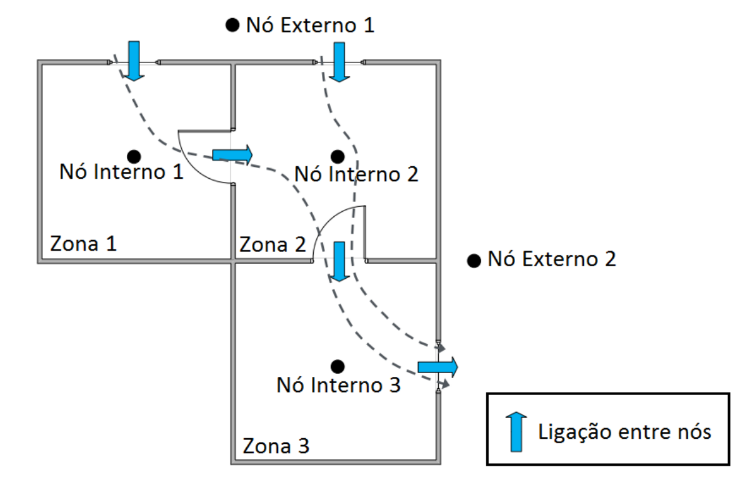
\includegraphics[width=.7\linewidth]{img/nos_AFN.png}
	\label{fig:nos_AFN}
	\source{adaptado de \citeonline{EnergyPlus2018}}
%	\begin{flushleft}
%		Fonte: adaptado de \citeonline{EnergyPlus2018}.
%	\end{flushleft}
\end{figure}

A velocidade na qual se considera que o vento atinge a edificação modelada é obtida a partir do arquivo climático utilizado na simulação computacional. A partir das medições de velocidade do vento na estação meteorológica, extrapola-se os valores para outras altitudes e perfis de terreno. Essa consideração em relação à velocidade do vento é baseada no \textit{Handbook of Fundamentals} da \citeonline{ASHRAE2005}.
Os coeficientes do perfil de velocidade do vento são variáveis que dependem das características de rugosidade do terreno no entorno. Os valores típicos são apresentados na Tabela \ref{tab:ventoterreno}.

\begin{table}[h]
	%		\vspace{-10pt}
	\caption{Coeficientes do perfil de velocidade do vento}
	\label{tab:ventoterreno}
	\centering
	\resizebox{\textwidth}{!}{
		\begin{tabular}{|c |c |c |c | } % \textwidth}{@{\extracolsep{\fill}} \hspace{-.33\columnwidth}
			\hline	
%			\textbf{Categoria} & {} & \textbf{Expoente,} & \textbf{Espessura da camada} \\
%			\textbf{do terreno} & {} & \textbf{$\alpha$} & \textbf{limite, $\delta$ ($m$)} \\
%			\hline	
			\textbf{Categoria} & {} & \textbf{Expoente,} & \textbf{Espessura da camada} \vspace{-5pt} \\
			{} & \textbf{Descrição do terreno} & {} & {} \vspace{-7pt} \\
			\textbf{do terreno} & {} & \textbf{$\alpha$} & \textbf{limite, $\delta$ ($m$)} \\
			\hline
			{} & Grandes centros urbanos nos quais & {} & \\
			1 & pelo menos 50\% das edificações são & 0,33 & 460 \\
			{} & maiores que 21 m. & {} & \\
			\hline
			{} & Terreno urbano, subúrbio, áreas com & {} & \\
%			2 & árvores, áreas com espaçamento & 0,22 & 370 \\

			{} & árvores, áreas com espaçamento & {} & {} \vspace{-5pt} \\ 
			2 & {} & 0,22 & 370 \vspace{-7pt} \\ 
%			
%			
%			{} & árvores, áreas com espaçamento & {} & {} \vspace{-2pt} \\ 
%			2 & {} & 0,22 & 370 \vspace{-3pt} \\ 
			
			{} & entre obstruções do tamanho ou & {} & \\
			{} & maiores do que casas unifamiliares. & {} & \\
			\hline
			{} & Terreno aberto com poucas & {} & \\
			3 & obstruções, geralmente menores do & 0,14 & 270  \\
			{} & que 10 m de altura. & {} & \\
			\hline
			{} & Área desobstruída plana exposta ao & {} & \\
			4 & vento. Entorno de corpos d’água de & 0,10 & 210  \\
			{} & mais de 1,6 km. & {} & \\
			\hline
			
		\end{tabular}
	}
	\source{adaptado de \citeonline{ASHRAE2005} (tradução do autor)}
%	\begin{flushleft}
%		Fonte: adaptado de \citeonline{ASHRAE2005} (tradução do autor).
%	\end{flushleft}
	%		\vspace{-12pt}
\end{table}

Os valores padrão para \gls{alphamet} e \gls{deltamet}, a partir dos quais se estima a velocidade do vento, são 0,14 e 270 m, respectivamente. Isso se deve ao fato de que estações meteorológicas são tipicamente estabelecidas em terrenos de categoria 3. A altura padrão é 10 m. 

Ao definir a velocidade do vento, o programa EnergyPlus calcula a pressão do vento sobre as edificações, determinada também pelo princípio da equação de Bernoulli \cite{Walton1989}.

A maior dificuldade no desenvolvimento do \acrshort{afn} é a necessidade de estimar as características do fluxo nas aberturas e o coeficiente de pressão do vento na edificação \cite{Arendt2017}. Os \acrfull{cp} descrevem como o vento interfere na distribuição externa de pressões em volta da edificação. 
De acordo com \citeonline{Costola2010}, os \acrshort{cp} se definem de acordo com Equação \ref{eq:CalcCp} e Equação \ref{eq:Pvel}.

%	\vspace{-8pt}
\begin{equation}\label{eq:CalcCp}
C_p = \frac{P_x - P_{\infty}}{P_d}
\end{equation}
%	\vspace{-5pt}
%	\vspace{-8pt}
\begin{equation}\label{eq:Pvel}
P_d = \frac{\rho V^{2}_{\infty}}{2}
\end{equation}
%	\vspace{-5pt}

Onde:

\gls{cpp} é o coeficiente de pressão ($-$);

\gls{px} é a pressão estática em um dado ponto da fachada do edifício ($Pa$);

\gls{p0} é a pressão estática no ambiente externo ($Pa$);

\gls{pd} é a pressão dinâmica ($Pa$);

\gls{rho} é a densidade do ar ($kg/m^3$);

\gls{vref} é a velocidade do vento no ambiente externo ($m/s$).
\\

Os \acrshort{cp} dependem principalmente da geometria da edificação, dos detalhes da fachada, do entorno da edificação, da velocidade e direção do vento, e da intensidade da turbulência. Na prática, destaca-se a dificuldade em determinar precisamente a relação entre o \acrshort{cp} e todos esses fatores. As abordagens mais realistas são os experimentos em escala real \textit{in-situ}. No entanto, esses experimentos possuem custo elevado e normalmente possuem grandes incertezas. 
Os dados dos \acrshort{cp} podem ser estimados pelas seguintes fontes: testes de túnel de vento; simulações com \acrshort{cfd}; modelos analíticos; e bases de dados.
Bases de dados de \acrshort{cp} são compilações de uma ou mais fontes, onde os dados são classificados de acordo com alguns parâmetros, como a forma da edificação e a orientação de incidência do vento. 

A dificuldade em se considerar toda a complexidade de variação do \acrshort{cp} faz com que os programas de simulação termoenergética de edificações com \acrshort{afn}, geralmente, incorporem métodos simplificados \cite{Costola2009}. Os experimentos de túnel de vento são as fontes primárias mais comuns. A qualidade dos resultados de túneis de vento são diretamente afetados pela calibração do túnel de vento, a garantia de qualidade dos procedimentos, e o conhecimento do pessoal para a preparação e execução dos testes.

Os túneis de vento permitem um bom grau de controle sobre os experimentos, assim como a repetitividade e reprodutibilidade dos testes conduzidos \cite{Omrani2017}. No entanto, a escala pode afetar o fluxo de ar e as transferências de calor se os parâmetros adimensionais corretos não são mantidos entre os modelos de diferentes tamanhos. Isso faz com que o ideal seja usar modelos em escala real.

Em casos em que não é possível obter os valores de \acrshort{cp} por fontes primárias, \citeonline{Costola2009} apontam as bases de dados como as fontes secundárias mais comuns.
A base de dados de pressão de vento da \acrfull{tpu} oferece dados experimentais obtidos a partir de experimentos em túnel de vento \cite{TPU2018}.
A base de dados possui os resultados de testes conduzidos utilizando-se modelos de acrílico em um túnel de vento de seção de 2,2 m de largura por 1,8 m de altura.
A camada limite atmosférica foi simulada por elementos geradores de turbulência e outros elementos de rugosidade. Diferentes perfis de vento foram usados para construir a base de dados. Na maioria dos experimentos a velocidade média e os perfis de intensidade de turbulência estavam de acordo com as de terreno suburbano. A intensidade de turbulência à altura de 10 cm foi cerca de 0,25, e a velocidade de vento teste a essa altura foi 7,4 m/s. O número mínimo de Reynolds foi 25340, que é acima do limite 11000 para o fluxo independente.
A base de dados da \acrshort{tpu} oferece valores de \acrshort{cp} para modelos de edificações com geometrias de diferentes proporções. Para cada modelo, valores diferentes de \acrshort{cp} são disponibilizados para diversos pontos sobre suas superfícies. 
A localização dos pontos sobre as superfícies dos modelos é apresentada de acordo com o exemplo da Figura \ref{fig:TPU_points}. Na imagem, 240 pontos de medição se distribuem sobre um modelo de dimensões igual a 0,2 m x 0,1 m x 0,2 m. As linhas pontilhadas representam as arestas do modelo.


\begin{figure}[h]
	\centering
	\caption{Distribuição de pontos de medição dos $C_p$ sobre a fachada}
	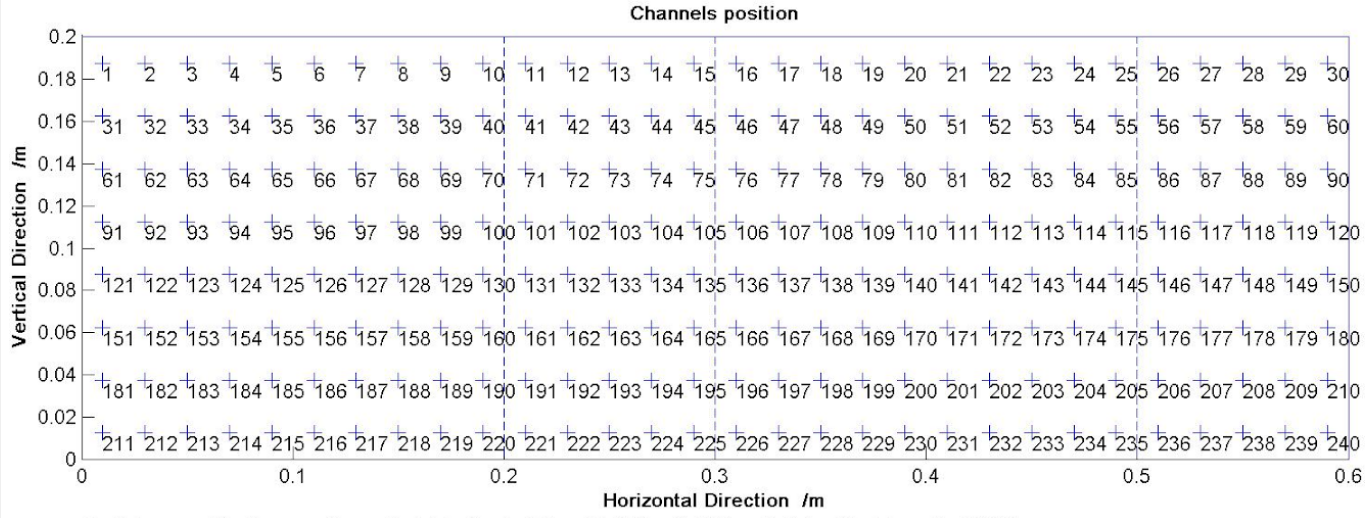
\includegraphics[width=1\linewidth]{img/tpu_points.png}
	\label{fig:TPU_points}
	\source{\citeonline{TPU2018}}
\end{figure}

Diversos fatores que afetam o valor do \acrshort{cp} são comumente simplificados, como apontado por \citeonline{Costola2010} na Tabela \ref{tab:CpSimp}.

\begin{table}[h]
	%		\vspace{-10pt}
	\caption{Fatores que afetam o $C_p$ e simplificações comuns}
	\label{tab:CpSimp}
	\centering
%	\resizebox{\textwidth}{!}{
		\begin{tabular}{|c |c |} % \textwidth}{@{\extracolsep{\fill}} \hspace{-.33\columnwidth}
			\hline	
			\textbf{Fatores que afetam o \acrshort{cp}} & \textbf{Simplificações comuns} \\
			\hline
			Ponto de interesse na superfície da & Dado médio para a superfície \\
			fachada da edificação (\acrshort{cp} local) & (\acrshort{cp} médio)\\
			\hline
%			Perfil do vento & Adoção de coeficientes que determinam \\
			{} & Adoção de coeficientes que determinam \vspace{-5pt}\\
			Perfil do vento & {} \vspace{-7pt}\\
			{} & o perfil de vento de acordo com o local \\
			\hline
			Elementos de obstrução da edificação & Obstruções com formas genéricas  \\
			\hline
%			Geometria da edificação e detalhes & Dados genéricos usados para \\
%			da fachada & qualquer forma, e sem detalhes na \\
%			{} & fachada considerados \\
%			\hline
			{} & Dados genéricos usados para \vspace{-5pt} \\
			Geometria da edificação e detalhes & {} \vspace{-7pt} \\
			{} & qualquer forma, e sem detalhes na \vspace{-5pt} \\
			da fachada & {} \vspace{-7pt} \\
			{} & fachada considerados \\
			\hline
			Direção do vento & Resolução angular baixa \\
			\hline
			
		\end{tabular}
%	}
	\source{adaptado de \citeonline{Costola2010} (traduzido pelo autor)}
	%		\vspace{-12pt}
\end{table}

Nas simulações termoenergéticas de edificações, há muita incerteza relacionada ao \acrshort{cp}. Isso deve-se à influência do \acrshort{cp} em muitos dos indicadores de desempenho, como consumo de energia ou conforto térmico, que são frequentemente sensíveis à vazão de ar \cite{Costola2009}. 
As bases de dados de \acrshort{cp} são amplamente disponíveis, particularmente para o cálculo de carga de vento em estruturas. Esses valores de \acrshort{cp} para edificações sem obstruções, com geometria simples, podem ser utilizados quando experimentos em túneis de vento não são disponíveis. Uma abordagem similar é usada para bases de dados de ventilação e infiltração na literatura. Nenhuma das bases de dados e modelos analíticos lidam com os efeitos da topografia local, detalhes da fachada, ou informam a incerteza dos dados disponibilizados. Os efeitos das edificações do entorno são considerados com muitas limitações e simplificações.

O estudo de \citeonline{Costola2010} quantifica a incerteza na vazão de ar devido ao uso do \acrshort{cp} médio da fachada, considerando 15 formas de edifícios e diferentes configurações de aberturas. O foco se deu em ventilação e infiltração movidas por vento, e a força de empuxo não foi considerada. Este estudo apresentou a estimativa de incerteza para edificações com duas aberturas idênticas, e uma zona interna, baseando-se em uma grande faixa de formas e ângulos de incidência do vento. A incerteza na vazão de ar calculada utilizando-se os coeficientes médios da superfície para edificações isoladas com duas aberturas varia entre 0,23 e 5,05 vezes o fluxo se comparada ao uso do \acrshort{cp} local, para um intervalo de confiança de 95\%. As grandes incertezas relativas devem-se às pequenas taxas de fluxo de ar. Quando se considera apenas as superfícies com maiores diferenças de pressão relativa, a incerteza diminui para  valores entre 0,52 e 1,42 vezes. Conclui-se que a magnitude da incerteza é alta, mas o julgamento em relação à aplicabilidade desses dados depende do problema em análise e do indicador de desempenho escolhido.

O trabalho de \citeonline{Arendt2017} estuda a influência dos dados de \acrshort{cp} de diferentes fontes na precisão de um modelo \acrshort{afn}. Uma edificação real com um sistema de ventilação movido por vento e força de empuxo foi adotado para um estudo de caso. Oito casos com diferentes dados de \acrshort{cp} foram estudados. Os resultados de temperatura do ar e fluxo do ar interno foram então comparados com as medições na escala real. Uma edificação residencial de dois pavimentos, localizada em Skarszewy, no norte da Polônia, foi escolhida para o estudo de caso. A edificação possui janelas e chaminés de ventilação. A densidade de construção na área de entorno da edificação não foi especificada no estudo. As simulações foram efetuadas para um período de tempo de 7 dias no fim da primavera. 
A modelagem da edificação foi realizada através do programa EnergyPlus 8.1 \cite{EnergyPlus2015}. Os valores de \acrshort{cp} foram obtidos de duas fontes: CPCALC+, que é um modelo analítico; e \acrshort{aivc}, que oferece uma base de dados. A partir dos dados do \acrshort{aivc}, considerou-se duas possibilidades: área plana aberta; e área rural com barreiras de vento espalhadas. A partir do CPCALC+ considerou-se as seguintes densidades de construção: 1\%, 10\% e 20\%. Para cada densidade de construção utilizada,considerou-se mais um caso onde o \acrshort{cp} para o ângulo de incidência de 180$^{\circ}$ teve seu valor alterado em -0,1. Essa foi uma variação arbitrária para verificar a influência nos resultados, uma vez que 180$^{\circ}$ era a direção de incidência predominante do vento no local. Em todos os casos considerou-se o \acrfull{cd} das aberturas igual a 0,6. 
Os casos mais precisos foram: o que considerou os valores da \acrshort{aivc} para terrenos com barreiras esparsas; e o que considerou os valores do CPCALC+ para 1\% de densidade, e variação de -0,1 no \acrshort{cp} para o ângulo de incidência de 180$^{\circ}$. O caso mais próximo do real obteve uma diferença relativa de 10\%, enquanto o pior caso (CPCALC+ 1\% de densidade) obteve um erro relativo de 169\%. Os erros do CPCALC+ foram maiores do que o do \acrshort{aivc}, mesmo considerando-se o \acrshort{cp} para a posição exata da abertura, enquanto o \acrshort{aivc} considerou a média na superfície da fachada. Nos melhores resultados, a diferença calculada para a temperatura do ar foi menor do que 0,5 $^{\circ}$C, enquanto nos piores, foi entre 1,1 $^{\circ}$C e 1,2 $^{\circ}$C. A correlação entre a precisão relativa do fluxo de ar e da temperatura do ar não foi linear. A conclusão final foi que simulações com \acrshort{afn} na fase inicial de projeto, quando não há dados experimentais disponíveis para a validação do modelo, possuem significantes incertezas.

\citeonline{Freire2013} avaliaram diferentes modelos de ventilação cruzada e unilateral (\textit{British Standard}, Gids e Phafe, e Larsen) e compararam com resultados de medições \textit{in-situ} e em túneis de vento. Também foram avaliadas as bases utilizadas para obtenção dos \acrshort{cp}. 
O modelo de Larsen mostrou-se mais apropriado para a ventilação unilateral, por considerar variações em função do ângulo de incidência do vento. Os \acrshort{cp} do CPCALC (\acrshort{cp} local) obtiveram resultados mais precisos do que os das equações de \citeonline{Swami1988} (\acrshort{cp} médio), que é o método padrão do programa EnergyPlus \cite{EnergyPlus2018} para a obtenção do \acrshort{cp}. Porém, ambos obtiveram erros relativos por volta de 30\%.

O fluxo de ar por grandes aberturas envolve diferentes obstáculos, que inclui desde fluxos gravitacionais estáveis, até fluxos flutuantes devido à turbulência do vento. A solução utilizada pelo programa EnergyPlus 8.9 \cite{EnergyPlus2018} para a modelagem de grandes aberturas é baseada no modelo COMIS \cite{Feustel1990}. As principais premissas para esse modelo são:

\begin{itemize}
	\item fluxo estável, fluido não-viscoso e incompressível;
	\item estratificação linear da densidade em ambos os lados da abertura;
	\item efeitos de turbulência representados por um perfil de diferença de pressão equivalente;
	\item efeitos de redução da área efetiva de abertura representados por um coeficiente.
\end{itemize}

O componente \textit{Detailed Opening} do EnergyPlus \cite{EnergyPlus2018} assume que, além da diferença de pressão entre os nós ligados pela abertura, há diferenças de pressão em função da altura da abertura, relacionadas à densidade do ar e à velocidade do vento. Por isso, é possível haver dois planos neutros de pressão ao longo da abertura, permitindo que o fluxo de ar se divida em três partes. 
Na Figura \ref{fig:DetailedOpening}, $P_{01}$ e $P_{02}$ representam as pressões nos nós, $\rho_{1}$ e $\rho_{2}$ representam funções que definem a diferença de densidade do ar em relação à altura, e $P_z$ representa uma função que define a diferença de pressão em relação à altura, causada pela turbulência do vento.


\begin{figure}[h]
	\centering
	\caption{Fenômenos considerado pelo EnergyPlus ao modelar fluxo de ar através de grandes aberturas}
	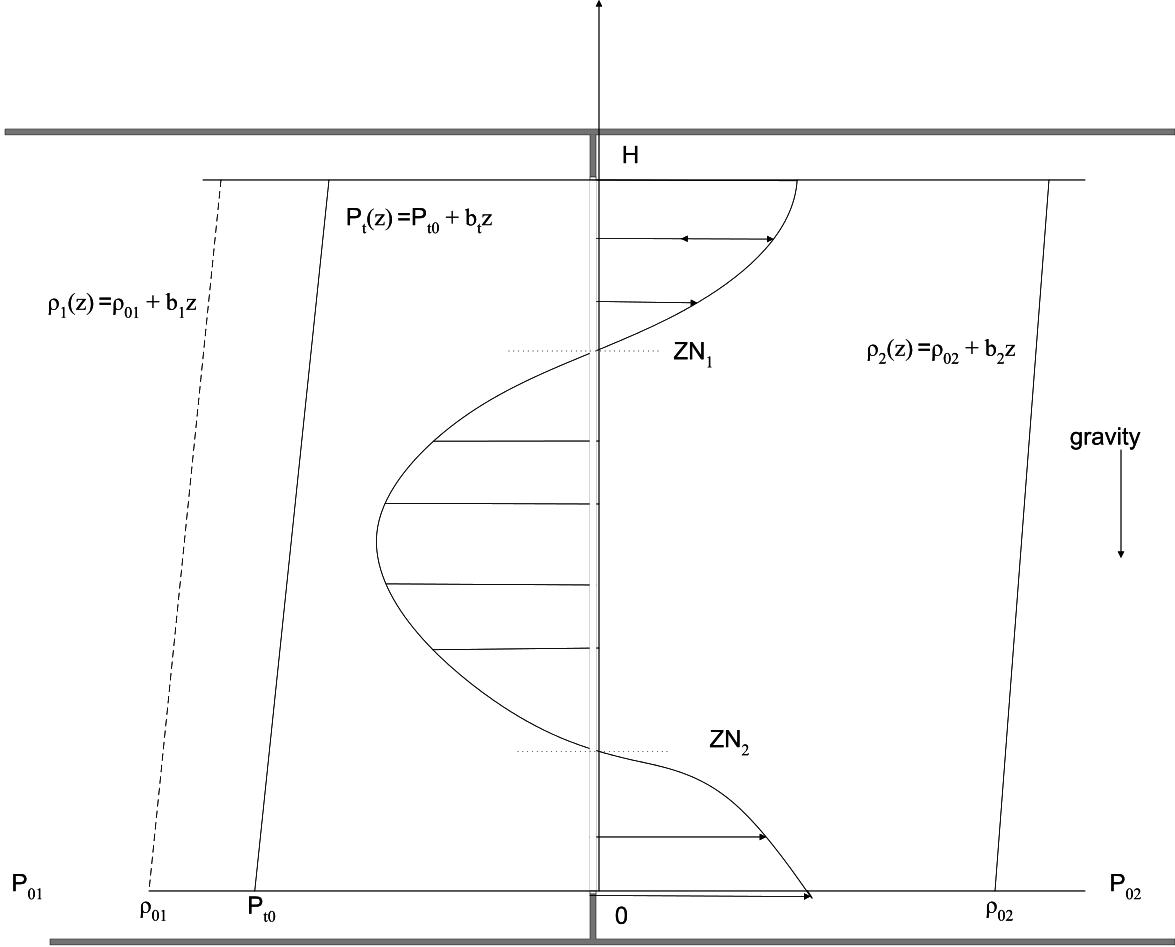
\includegraphics[width=\figsize\linewidth]{img/detailed_opening.png}
	\label{fig:DetailedOpening}
	\source{EnergyPlus2018}
%	\begin{flushleft}
%		Fonte: \citeonline{EnergyPlus2018}.
%	\end{flushleft}
\end{figure}

O \acrfull{cd} é utilizado para representar a característica do fluxo na abertura quando a abertura é grande. Para frestas, utiliza-se o coeficiente de fluxo mássico de ar (\acrshort{cq}) \cite{Arendt2017}.
Esses coeficientes são definidos como a razão entre o fluxo real em relação ao	ideal, quando a vazão mássica de ar de referência é definida para a diferença de pressão de 1 Pa. Ambos os parâmetros dependem da geometria da abertura, velocidade do ar, orientação geográfica, edificações do entorno, morfologia urbana e a forma do edifício em questão.
O valor do \acrshort{cd} é o produto entre o coeficiente de velocidade e o coeficiente de contração \cite{Flourentzou1998}. Ele pode ser determinado experimentalmente quando a vazão de ar é medida diretamente, com gás rastreador, por exemplo. O coeficiente de velocidade também pode ser determinado similarmente medindo-se as velocidades do ar.

\citeonline{Iqbal2015} apontam que o \acrshort{cd} representa os efeitos não ideais de fluxo, que são causados principalmente pela fricção no caminho do fluxo de ar e o efeito de contração devido a mudanças na direção do fluxo. Devido à dificuldade de se estimar esses efeitos separadamente, normalmente apenas o \acrshort{cd} é usado para especificar vazão de ar através de aberturas. O valor de \acrshort{cd} para janelas operáveis não é constante, mas varia consideravelmente de acordo com a área de abertura, o tipo de janela e a diferença de pressão entre a abertura. O uso de valores constantes de \acrshort{cd} podem levar a estimativas errôneas do fluxo de ar.

De acordo com o manual do COMIS \cite{Feustel1990}, os valores de \acrshort{cd} podem variar de 0,61, para orifícios de arestas vivas,	até 0,98 para tubos com forma de trompete. Os valores encontrados podem variar de 0,25 até 0,75 para grandes aberturas. Normalmente assume-se o valor de 0,6 para aberturas retangulares em simulações  \cite{Flourentzou1998, Heiselberg2001, Breesch2010, Iqbal2015, Krzaczek2015, Arendt2017}.

O objetivo de \citeonline{Flourentzou1998} foi identificar os valores de coeficientes de resistência de fluxo para uma edificação de escritórios de três pavimentos naturalmente ventilada na Suíça. A ventilação por força do vento foi desconsiderada devido à sua instabilidade, o que fez com que os experimentos fossem conduzidos em noites sem vento. O estudo considerou apenas ventilação por força de empuxo, de fluxo levemente turbulento, buscando validar algoritmos simples de ventilação e dar uma base experimental para diretrizes de projeto para técnicas de resfriamento noturno. Nos experimentos, mediu-se a velocidade do ar e linha de pressão neutra, observando-se os coeficientes de contração e de velocidade usados no modelo de Bernoulli. As medições foram efetuadas levando-se em conta a ventilação unilateral e cruzada. As escadas funcionaram como uma chaminé de exaustão nas trocas de ar por empuxo. Os valores de \acrshort{cd} encontrados estão de acordo com o valor geralmente aceito de 0,6 ${\pm}$ 0,1.

\citeonline{Heiselberg2001} descreveram e sumarizaram os resultados de uma série de medições em laboratório, desenvolvidas para determinar as características do fluxo de ar em janelas abertas, e da distribuição de ar na sala, além de fornecer dados para projetos. O trabalho focou na estimativa dos \acrshort{cd}, nas condições de fluxo de ar no ambiente e no desenvolvimento de um modelo semi-empírico de fluxo para estimar parâmetros de conforto em zonas ocupadas. As medições foram aplicadas a dois tipos de janelas, e em função do ângulo de abertura e diferenças de pressão e temperatura através da abertura. Os resultados mostram que o \acrshort{cd} não pode ser considerado constante, pois varia consideravelmente em função da área de abertura, do tipo de janela e das diferenças de temperaturas. Isso pode levar a erros relacionados à capacidade de fluxo. O valor normalmente adotado de 0,6 é obtido apenas para áreas de abertura grandes. Áreas de abertura menores possuem valores maiores.

O estudo de \citeonline{Iqbal2015} avalia o efeito do ângulo de abertura na vazão de ar em janelas pivotantes em telhados. Os valores de \acrshort{cd} são obtidos para os diferentes ângulos, com e sem vento, para fluxos de entrada e saída. Utilizou-se medições em túnel de vento para o estudo, com o modelo de uma residência em escala 1:20. Os resultados são apresentados para fluxo unidirecional. Na ausência de vento, o \acrshort{cd} diminui com o aumento do ângulo de abertura. O \acrshort{cd} mostrou-se variar em função do número de Reynolds. Para fluxo turbulento totalmente desenvolvido, o \acrshort{cd} também diminui com o aumento no ângulo de abertura. Para fluxos de ar movidos por vento, o \acrshort{cd} da janela depende da turbulência na vazão de ar que passa pela abertura. Concluiu-se que o valor de \acrshort{cd} varia em função da fração de velocidade (velocidade média do ar em relação à velocidade do vento de referência). Os valores de \acrshort{cd} para fluxos de entrada e saída foram diferentes. Quando a velocidade do ar é superior à velocidade do vento de referência, o \acrshort{cd} é independente da fração de velocidade e da direção do fluxo, e os valores de \acrshort{cd} são idênticos aos valores para velocidade do vento igual a zero. Para ângulos de abertura pequenos o \acrshort{cd} era próximo a 1, enquanto o valor mínimo de \acrshort{cd} foi igual a 0,6 para abertura máxima, valor geralmente utilizado nos modelos de \acrshort{afn} para grandes aberturas. Concluiu-se que janelas pivotantes podem auxiliar na obtenção de valores maiores para o \acrshort{cd}, que varia em relação ao ângulo de abertura.
%
%O fluxo de ar por aberturas horizontais no programa EnergyPlus 8.9 \cite{EnergyPlus2018} é baseado no trabalho de \citeonline{Cooper1989}. Considera-se fluxo de ar por diferença de pressão entre as zonas, por diferença de densidade (causada pelas diferenças de temperatura), ou ambos os fenômenos simultaneamente. A troca de ar total entre as zonas é a soma do fluxo gerado pela diferença de pressão, mais o fluxo da força de empuxo. Porém, o fluxo de ar que desce pela força de empuxo é igual ao fluxo de ar que sobe, cancelando a parcela da força de empuxo no somatório da massa de ar que entra e sai da zona. Para a modelagem de uma escada, há a possibilidade de se considerar um plano inclinado na abertura horizontal. Essa consideração é realizada pela substituição da área de abertura por uma área de abertura efetiva.

A \acrlong{vn} é um fenômeno complexo, dependente de diversos fatores. O uso de modelos \acrshort{afn} tem algumas limitações, assim como os coeficientes adotados para a aplicação dos modelos. Apesar das condições de contorno e simplificações adotadas, o \acrshort{afn} apresenta-se como uma solução mais compatível com programas de simulação termoenergética de edificações como o EnergyPlus, devido ao relativo baixo custo computacional e à integração já	existente aos demais algoritmos do programa.

\section{Conforto térmico}

Dentro de uma edificação, diversos fatores podem influenciar no conforto dos ocupantes, como características acústicas, visuais ou térmicas. Devido ao foco deste trabalho, serão discutidas questões relacionadas ao conforto térmico.
A busca por conforto térmico tem influência significativa na construção de edificações e na escolha dos materiais construtivos. Esse conforto depende de fatores físicos, fisiológicos e psicológicos. De acordo com a \citeonline{ASHRAEStandard552017}, conforto térmico é o estado da mente que expressa satisfação da pessoa com o ambiente térmico que a circunda, e é estimado através de avaliação subjetiva. No estudo do conforto térmico há duas abordagens principais: o modelo estático e o modelo adaptativo. % \textit{Standard 55}
O modelo estático foi desenvolvido por \citeonline{Fanger1970a}, a partir de estudos realizados em câmaras climatizadas. As câmaras climatizadas tinham temperatura, umidade relativa e velocidade do ar controladas, e os objetos de estudo exerciam atividades e utilizavam vestimentas específicas. Neste estudo, as variáveis mais importantes que influenciam no conforto térmico são: nível de atividade; resistência térmica das roupas; temperatura do ar; temperatura radiante média; velocidade do ar; umidade relativa no ambiente.

Para determinar o nível de conforto térmico no ambiente construído, \citeonline{Fanger1970a} desenvolveu a partir dessas variáveis o “Voto Médio Predito” (\acrshort{pmv}), uma escala para otimizar as condições de conforto térmico em um ambiente construído. A escala do \acrshort{pmv} prediz se os ocupantes do ambiente estarão sentindo frio, calor ou neutros. Para que haja conforto térmico, é necessário que haja neutralidade térmica. A neutralidade térmica é a condição na qual a pessoa prefere que o ambiente à sua volta não esteja nem mais frio, nem mais quente.

A abordagem no modelo adaptativo é diferente da proposta no modelo estático. \citeonline{Dear1997} afirmam que uma premissa importante do modelo adaptativo é que o ocupante da edificação não é simplesmente um receptor passivo de um dado ambiente térmico, como no caso das câmaras climáticas, mas em vez disso é um agente ativo, que interage em diversos níveis do sistema “pessoa-ambiente” via ciclos retroalimentados. As expectativas térmicas resultam da confluência de experiências correntes e passadas, e práticas técnicas e culturais. Sendo assim, leva-se em conta diferenças não apenas quantitativas, mas também qualitativas entre o conforto térmico em edificações condicionadas artificialmente e naturalmente ventiladas. Baseando-se em um estudo de um banco de dados de 21 mil medições realizadas em edificações comerciais, \citeonline{Dear1997} concluíram que, em edificações ventiladas naturalmente, a tolerância dos usuários em relação à variação de temperatura é maior, e o conforto depende diretamente das temperaturas médias externas.

A \citeonline{ASHRAEStandard552017} define os limites inferior e superior de temperatura operativa do ambiente, para 80\% de aceitabilidade, em ambientes ventilados naturalmente, a partir das Equações \ref{eq:limInf} e \ref{eq:limSup}.

%	\vspace{-8pt}
\begin{equation}\label{eq:limInf}
T_{inf} = 14,3 + 0,31 T_m
\end{equation}
%	\vspace{-5pt}
%	\vspace{-8pt}
\begin{equation}\label{eq:limSup}
T_{sup} = 21,3 + 0,31 T_m
\end{equation}
%	\vspace{-5pt}`

Onde:

\gls{tinf} é o limite inferior da temperatura operativa para que haja conforto térmico ($^{\circ}C$);

\gls{tsup} é o limite superior da temperatura operativa para que haja conforto térmico ($^{\circ}C$);

\gls{tm} é a temperatura média do ar no ambiente externo ($^{\circ}C$).
\\

A temperatura média do ar externo representa o ambiente climático externo com o qual os ocupantes da edificação estão fisiologicamente,
comportamentalmente e psicologicamente adaptados. Essa variável de entrada é baseada na média aritmética das temperaturas médias externas diárias em um período de dias, e pode ser considerada como a temperatura média mensal.

O movimento do ar influencia no conforto térmico, causando desconforto por frio em algumas situações, mas também reduzindo o desconforto por calor.
Isso ocorre devido ao aumento da convecção sobre as superfícies, o que causa maior evaporação, fenômeno endotérmico. Devido a essa influência no conforto térmico, a \citeonline{ASHRAEStandard552017} permite considerar a velocidade do ar como um fator determinante na busca por um ambiente termicamente confortável. Essa consideração é baseada nos valores do  \textit{Standard Effective Temperature} (SET), que relaciona a velocidade do ar e a temperatura operativa do ambiente para ambientes climatizados.

\citeonline{DeVecchi2015} aplicaram o método adaptativo da \citeonline{ASHRAEStandard552013} para o contexto climático brasileiro, caracterizado como quente e úmido. Os resultados indicam que é possível encontrar níveis aceitabilidade térmica significativamente abaixo dos limites inferiores do método adaptativo. Essa tolerância a temperaturas mais baixas deve-se ao aumento de vestimentas por parte dos ocupantes, antes de se recorrer ao aquecimento artificial. Os autores sugerem que a fixação do limite inferior de temperatura operativa em no máximo 19,5 $^{\circ}$C, para umidade relativa de 80\%, representaria mais adequadamente o comportamento dos usuários no contexto climático brasileiro.

\section{Ventilação natural em edifícios de escritórios}

Nesta parte da revisão, buscou-se identificar estudos sobre o uso da \acrshort{vn} em edificações de escritórios. Foram identificadas as características dos edifícios relacionadas à geometria, envoltória, padrões de uso, ganhos internos, configuração das aberturas da fachada, entre outros.

Ao longo da maior parte da história, as edificações eram projetadas de forma que o potencial da \acrshort{vn} fosse explorado ao máximo. Com a invenção do ar condicionado, a partir da segunda metade do século 20, houve um crescimento do uso de ventilação mecânica e condicionamento de ar no mundo e, com isso, a arquitetura das edificações comerciais começou a sofrer mudanças \cite{CarrilhodaGraca2016}. Associado a essas mudanças do desenho vernacular tradicional, o desenvolvimento urbano resultou em problemas particulares relacionados à demanda de resfriamento nos meses mais quentes. Os grandes centros urbanos são considerados como uma ilha de poluição. Em muitas cidades, o ambiente externo é contaminado com ruído sonoro, partículas finas, calor e gases tóxicos. A dificuldade na aplicação da \acrshort{vn} em edifícios comerciais atualmente se deve ainda a aspectos como a necessidade da concepção do conceito desde as fases iniciais de projeto, ou até mesmo a questões estéticas.

A intensidade de ocupação em edifícios de escritórios varia de acordo com as atividades exercidas. Alguns escritórios são continuamente ocupados por computadores e equipamentos ligados constantemente, enquanto outros são pouco ocupados e têm pouco uso de computadores e iluminação \cite{Elharidi2018}.

\citeonline{Neves2019} desenvolveram um banco de dados com informações levantadas em edifícios de escritórios que operam com ventilação híbrida (\acrshort{vn} e condicionamento artificial de ar). Para isso, 153 edifícios construídos após o ano de 1995 na cidade de São Paulo foram selecionados. Dentre os edifícios selecionados, foi realizado um levantamento de campo em 50 edifícios, obtendo-se informações relacionadas às dimensões das salas de escritórios, ao tipo de esquadria utilizado e à presença de elementos de sombreamento. As informações disponíveis em todos os edifícios do banco de dados incluem: áreas, dimensões, formato e número de pavimentos das edificações; absortância das paredes externas e coberturas; e \acrfull{paf}. Os autores observaram as correlações entre as características encontradas nestes edifícios. As estratégias de \acrshort{vn} adotadas não parecem ser algo que procura-se otimizar nos projetos dos edifícios analisados. Tampouco há indicação de uma mudança nesse cenário em edificações de anos mais recentes. O que se nota é o aumento de elementos de sombreamento na fachada em razão do uso de equipamentos condicionadores de ar do tipo \textit{split}. Os autores concluem que o levantamento realizado permite a identificação das características mais recorrentes nos edifícios analisados, e os intervalos de variação nos parâmetros observados.
Isso possibilita que trabalhos relacionados ao desempenho térmico de edificações sejam desenvolvidos considerando-se características de edificações reais.

\citeonline{Belleri2014} compararam predições de desempenho de \acrshort{vn} em estágio inicial de projeto pelo programa EnergyPlus com medições de campo. O escritório estudado localiza-se no segundo andar de um edifício de dois andares na Califórnia, Estados Unidos, e tem seu espaço dividido em dois planos abertos de 130 m$^2$, conectados por duas grandes aberturas. Não há ventilação forçada ou sistema de resfriamento. As quatro fachadas são providas de janelas, que podem ser operadas pelos ocupantes. Há ventiladores de teto com controle variável disponíveis. Os autores partiram da simulação de um modelo simples, e modificaram gradativamente os seguintes dados de entrada, de acordo com medições em campo: temperaturas internas; controle das janelas; dados climáticos (com intervalos de 5 minutos); fatores de abertura das janelas, coeficientes de pressão do vento (baseados em medições em túnel de vento). Enquanto a simulação inicial superestimou a média das trocas de ar em 1671\%, a simulação com todas as modificações superestimou as trocas de ar em apenas 148\%. O estudo conclui que, com dados suficientes, a utilização do programa EnergyPlus com o \acrshort{afn} pode oferecer  estimativas informativas relacionadas ao desempenho da \acrshort{vn}. No entanto, para melhores estimativas é necessário obter dados relacionados ao vento e ao comportamento dos ocupantes, o que pode ser inviável na fase de projeto.

O trabalho realizado por \citeonline{Elharidi2018} buscou identificar o desempenho energético e a qualidade do ar interno de edifícios de escritórios no Egito, propondo medidas para minimizar o uso de energia. Os dados foram levantados a partir de questionários realizados em 59 escritórios, sendo complementados por dados da literatura. Os dados registrados incluem: área interna, atividade exercida no escritório, tipo de serviço prestado na edificação, tipo de edificação, e contas de energia elétrica. Dentre as atividades nos escritórios, inclui-se contadores, agências de viagem, vendas, administração da saúde, seguros, consultores, administração de bancos, recursos humanos, e governo. As edificações de escritórios foram classificadas em quatro tipos: \acrshort{vn} sem resfriamento; \acrshort{vn} com resfriamento local; ventilação mecânica com resfriamento local; ventilação mecânica e resfriamento central. A maioria das edificações estudadas possui apenas \acrlong{vn}, ou \acrshort{vn} com resfriamento local. A estratégia adotada para resfriamento e ventilação dos edifícios foi identificada como o fator mais impactante no consumo de energia. A eficiência dos equipamentos, iluminação e sistemas de resfriamento, relacionada ao comportamento dos ocupantes, pode reduzir significativamente o consumo elétrico da edificação. 
Os edifícios com apenas \acrshort{vn} têm os menores consumos de energia, sendo que há a possibilidade de desconforto térmico em certas épocas do ano sob essas condições. Os edifícios com \acrshort{vn} e resfriamento local têm maior consumo de energia nos meses de verão, mas demandam menos da metade do consumo de energia dos edifícios com resfriamento central.

O estudo de \citeonline{Roetzel2014} investigou o impacto do projeto da edificação e da ocupação no conforto térmico e desempenho energético em escritórios, para identificar padrões que ajudem nas considerações relacionadas aos estágios iniciais de projeto. O estudo baseia-se no cenário A2 do \textit{International Panel on Climate Change} (IPCC), para o ano de 2030.
Uma sala de escritório celular foi modelada e simulada para três climas através do programa EnergyPlus. Os locais considerados são: Hamburgo, Alemanha; Atenas, Grécia; e Alice Springs, Austrália. Dentre as variações no projeto, considerou-se três tipos de construções: de luxo; de baixo custo inicial; e sustentável. As considerações relacionadas ao comportamento dos ocupantes foram duas: de pior cenário; e de cenário ideal. Para avaliar o conforto térmico e o desempenho energético, as simulações foram realizadas para duas condições: sem consideração de resfriamento e aquecimento para análise de conforto; e incluindo-se \textit{setpoints} para aquecimento e resfriamento.
O estudo conclui que os comportamento dos ocupantes é o que mais influencia no consumo final de energia para todos os climas investigados.
Para buscar um melhor desempenho e melhores níveis de conforto, as seguintes estratégias para o projeto da edificação são indicadas: proteção solar externa que permita iluminação natural; \acrshort{paf} maiores que 70\% e janelas localizadas acima do plano de trabalho; massa térmica aplicada ao piso, paredes e cobertura. Em relação ao comportamento dos ocupantes, as estratégias sugeridas são: operar ativamente as janelas durante o dia e também para a ventilação noturna; operar venezianas para aproveitar a iluminação natural, prevenindo-se de ofuscamento e calor; operar iluminação artificial dependendo da luz natural; e utilizar equipamentos de escritório com baixa potência de consumo.

\citeonline{Pesic2018} descrevem a aplicabilidade geoclimática da \acrshort{vn} na região da Catalunha, na costa do Mediterrâneo. O objetivo é providenciar diretrizes e parâmetros básicos de eficiência energética para arquitetos, engenheiros e políticos, para que possam visualizar o potencial da \acrshort{vn}. Três cidades foram analisadas: Barcelona; Terrassa; e Tarragona. O modelo de escritório representa um edifício de três pavimentos \textit{open-plan}. A ventilação cruzada é modelada considerando-se a passagem de ar por janelas operáveis, com movimento gerado primariamente por força do vento. A orientação da edificação foi definida perpendicularmente à principal direção do vento nos meses em que a \acrshort{vn} é mais favorável. O \acrshort{paf} é definido como 40\% e a infiltração na envoltória é considerada constante, com 0,25 \acrfull{ach} por hora. As temperaturas limite de aceitabilidade do ar externo para \acrshort{vn} são entre 10 $^{\circ}$C e 33,5 $^{\circ}$C. O horário de ocupação é das 8h00 às 18h00, e a ventilação noturna é das 21h00 às 7h00. Considerou-se a possibilidade de uso de condicionamento de ar para aquecimento e resfriamento, ou ventilação mecânica (\acrshort{hvac}) entre as 6h00 e 18h00. A ocupação foi considerada apenas durante os dias de semana. A construção e isolamento da edificação foram definidos de acordo com os padrões da Passivhaus, padrão de construção baseado no uso de isolamento térmico da edificação. A \acrshort{vn} foi considerada entre os dias 1º de abril e 31 de outubro (meses quentes). Seis modos de resfriamento foram considerados na análise: apenas \acrshort{hvac}; \acrshort{vn} ou \acrshort{hvac}; \acrshort{vn} ou \acrshort{hvac}, e ventilação noturna; \acrshort{vn} e \acrshort{hvac} simultaneamente; \acrshort{vn} e \acrshort{hvac} simultaneamente, e ventilação noturna; apenas ventilação noturna. O maior potencial de redução de energia foi observado para o uso simultâneo de \acrshort{hvac} e \acrshort{vn}, com ventilação noturna. Em relação ao caso com apenas \acrshort{hvac}, a redução relativa foi de 28,4\%, em Tarragona, a 40,9\%, em Barcelona.

O estudo de \citeonline{Yao2009} buscou um método de analisar estrategicamente o uso de \acrshort{vn} nas etapas iniciais de projeto. Consideraram-se as condições climáticas locais, tipo de edificação, padrões de ocupação e ventilação. O trabalho é desenvolvido a partir de um modelo de escritório para cinco climas da China: muito frio; frio; verão quente e inverno frio; verão quente e inverno ameno; e ameno. Os escritórios na China se dividem em dois tipos principais: de alto padrão com sistema central de ar condicionado; e escritório tradicional com ar condicionado \textit{split}. O modelo de escritório utilizado para o estudo possui as seguintes características: sala com dimensões 3,6 m x 5,4 m x 3,0 m; orientação sul-norte; \acrshort{paf} de 0,35 na parede sul e 0,25 na parede norte; ocupação das 8h00 às 18h00; capacidade térmica média; elementos de sombreamento interno na fachada sul no verão; tipo de terreno urbano; ganhos internos igual a 25 W/m$^2$. Os autores concluem que em zonas de clima ameno a \acrshort{vn} é altamente recomendável para edifícios de escritório em ambos os turnos. A ventilação cruzada tem maior eficiência do que a ventilação unilateral.
Em zonas de verão quente e inverno ameno, o uso de \acrshort{vn} não satisfaz as exigências para conforto térmico. Portanto, o resfriamento mecânico é recomendado. Observou-se que o uso unicamente da ventilação noturna não é adequada para edifícios de escritórios, pois os ganhos internos gerados ao longo do dia não podem ser liberados, causando desconforto térmico. 

\citeonline{Yun2008} comentam a dificuldade de se modelar o comportamento dos ocupantes, e como esse aspecto é uma barreira na exploração do uso de técnicas passivas e mistas de eficiência energética. Um estudo de caso foi conduzido durante o verão em seis salas de escritório com \acrshort{vn}, localizados em Cambridge, Reino Unido. Os escritórios são ocupados por uma ou duas pessoas, e têm o \acrshort{paf} variando entre 0,12 e 0,57. Dentre os objetivos do estudo, buscou-se examinar o potencial da \acrshort{vn} como estratégia de conforto e resfriamento. Foram coletados dados relacionados à posição das janelas e temperaturas internas e externas, além da aplicação de questionários.
Dos casos analisados, o que obteve melhor índice de conforto foi o escritório com brise externo e com possibilidade de aplicação de ventilação noturna. O caso com maior desconforto por calor possui uma janela com \acrshort{paf} de 0,57 orientada para oeste, sem sombreamento externo. As análises mostram que elementos do projeto como a orientação da fachada, o tamanho da janela em relação à orientação, a possibilidade de \acrlong{vn} pela janela, e o sombreamento externo por brise ou edificações vizinhas são fatores determinantes no desempenho térmico. Os autores apontam que áreas envidraçadas menores podem melhorar o desempenho térmico, mas podem comprometer o uso da iluminação natural. Portanto, é crucial buscar um equilíbrio entre o uso de iluminação natural e a busca por minimizar os ganhos de calor pela fachada. Os resultados sugerem que a \acrshort{vn} como um método de resfriamento passivo nem sempre é efetiva, pois os ocupantes nem sempre operam as janelas de acordo com as condições ideais para o resfriamento por ventilação. Portanto, destaca-se a importância de se elaborar um projeto robusto para a edificação, para compensar comportamentos desfavoráveis por parte dos ocupantes.

De acordo com \citeonline{CarrilhodaGraca2016}, nos climas quentes, que é o caso do Brasil, há maior potencial de economia e maior desafio na aplicação de \acrshort{vn}. \citeonline{Roetzel2014} afirmam que o modelo adaptativo da \citeonline{ASHRAEStandard552017} tem uma faixa maior de aplicabilidade em climas mais quentes, o que pode propiciar um maior potencial de otimização.
Esta parte da revisão bibliográfica apresentou estudos que abordam o potencial de \acrshort{vn} como uma solução para o resfriamento passivo em edificações de escritórios. Nos diferentes casos e configurações dos sistemas de resfriamento considerados, algumas características avaliadas e soluções propostas são predominantes, como o uso de ventilação cruzada ou de sombreamento das aberturas.
No entanto, a variação de determinadas características das edificações podem resultar em desempenhos térmicos diferentes de acordo com as combinações de parâmetros, ou características climáticas. 

\section{Análise de sensibilidade}

\Acrfull{as} é uma ferramenta valiosa na simulação termoenergética de edificações. Por isso, a \acrshort{as} é usada amplamente para explorar as características do desempenho térmico em edificações em diversas aplicações, como projetos, calibração de modelos, \textit{retrofits}, impacto das mudanças climáticas, entre outros \cite{Tian2013a}. A metodologia para a aplicação da \acrshort{as} tipicamente adota os seguintes passos: determinar as variações dos dados de entrada; determinar os modelos das edificações; executar as simulações dos modelos; coletar os resultados; executar a \acrshort{as}; apresentar os resultados da \acrshort{as}. Os métodos de \acrshort{as} podem ser divididos entre as abordagens local e global. A \acrshort{as} local é focada nos efeitos da incerteza de parâmetros de entrada em torno de um caso base, enquanto a \acrshort{as} global é mais interessada na influência dos parâmetros de entrada sobre todo o espaço de parâmetros de entrada possíveis. Por isso, a \acrshort{as} global é considerada mais confiável. A \acrshort{as} global inclui métodos de regressão, baseados em screening, em variância e metamodelos.

O primeiro passo para realizar uma \acrshort{as} é determinar a faixa dos dados de entrada. Quando o objetivo é determinar diferentes opções de projeto,  \citeonline{Tian2013a} sugere distribuições uniformes nos dados de entrada, pois assume-se que os diferentes valores para os dados de entrada são igualmente prováveis.

O método da variância decompõe a incerteza dos dados de saída para seus correspondentes dados de entrada  \cite{Tian2013a}. Nessa abordagem, os dois métodos mais comuns são o FAST \cite{Saltelli2004} e o de \citeonline{Sobol1993}. 
Por esses métodos, é possível avaliar efeitos de primeira ordem e de ordens superiores.
Os efeitos de primeira ordem são determinados observando-se o quanto a variância nos dados de saída dependem da variação de cada parâmetro, isoladamente.
Os efeitos de segunda ordem consideram as interações entre dois parâmetros na variância dos dados de saída, e a mesma lógica segue para os efeitos de ordens superiores.
Os efeitos totais, para cada parâmetro, são a soma dos efeitos de todas as ordens.
Ao somar os efeitos de primeira ordem mais os efeitos de ordens superiores, de todos os parâmetros do modelo, o valor obtido deve ser igual a 1.
Quando o objetivo é fixar parâmetros não impactantes nos resultados, os efeitos totais devem ser considerados \cite{Saltelli2004}. Métodos de variância são de abordagem livre, fazendo com que sejam adequados para modelos não-lineares e com correlações entre variáveis.

\section{Metamodelos de eficiência energética e desempenho térmico em edificações}
Projetistas encontram dificuldades no uso de ferramentas de simulação de desempenho energético, que podem não ser compatíveis com suas necessidades e métodos de trabalho. Por isso, \citeonline{Picco2014a} propõem simplificar a descrição do edifício e converter um modelo detalhado em um modelo simplificado, com apenas um número limitado de entradas. Em um estudo de caso, simplificações foram assumidas quanto às envoltórias, superfícies transparentes, zonas térmicas e pavimentos de um edifício comercial. As diferenças encontradas em relação ao modelo detalhado, no pior caso, foram de 15,6\% para cargas de aquecimento e 14,6\% para cargas de resfriamento. Com diferenças menores de 4\% e 9\% para cargas de pico, respectivamente. Apesar das margens de erro, os autores observaram que simplificações no modelo podem auxiliar em estágios iniciais de projeto, quando certas características no projeto do edifício ainda não estão bem definidas.

Há modelos baseados em equações físicas, que simulam os sistemas de transferência de calor, e modelos baseados em funções estatísticas, que deduzem esses comportamentos. Modelos estatísticos funcionam apenas com entradas e saídas, sem correlacionar causa e efeito, mas têm maior agilidade. 
Os modelos escritos com equações físicas seguem os princípios da conservação de energia e são os que mais se aproximam do comportamento real, mas podem ser dificultosos de se aplicar por serem complexos. Para adaptar as principais funcionalidades de ambos os modelos, existem modelos híbridos, chamados metamodelos.

Modelos preditivos são funções matemáticas que, aplicadas a uma quantidade significativa de dados, conseguem identificar padrões ocultos e prever o que poderá ocorrer. Os métodos de inteligência artificial mais utilizados para predição de desempenho energético de edificações são \acrfull{ann} e \acrfull{svm} \cite{Zhao2012}. São modelos altamente eficazes na solução de problemas não-lineares. Esses métodos podem oferecer predições altamente precisas, desde que as definições do modelo e parâmetros estabelecidos estejam definidos adequadamente. Modelos de \acrshort{ann} já foram usados para analisar vários tipos de consumo de energia em edificações em diversas condições, como em cargas de aquecimento e resfriamento, consumo de eletricidade, operação e otimização de componentes, e estimativa de parâmetros de uso. O uso de \acrshort{svm} vem crescendo em pesquisas e indústria. Em muitos casos as \acrshort{svm} mostram performances superiores às das \acrshort{ann}, mesmo com pequena quantidade de dados para treinamento.

Os resultados de simulações podem ser avaliados a partir de características específicas. Essas características podem incluir pico da demanda de energia, consumo anual de energia, conforto, custo do ciclo de vida, entre outros. No desenvolvimento de um metamodelo analítico para otimização de modelos de energia de edificações, \citeonline{Eisenhower2012} utilizaram o \acrshort{pmv} para a avaliação dos resultados. A caracterização dos dados e técnica de regressão do modelo foram baseadas em princípios de aprendizagem automática. Aprendizagem automática é uma classificação de algoritmos que tentam identificar características dentre os dados, sem conhecimento prévio dessas características. 
Dentre diferentes possíveis abordagens (\acrshort{ann}, Programação Genética, Redes Bayesianas) a escolhida para o caso foi a \acrshort{svm}. 
A identificação dos parâmetros mais influentes no processo de otimização foi realizada através de uma análise de sensibilidade global, baseada em derivadas locais. O metamodelo gerado foi capaz de identificar a minimização do consumo de energia, mantendo ou melhorando o conforto, sem necessidade de extensivas repetições de simulações de energia.

\citeonline{Rackes2016} propõem um metamodelo para analisar edificações comerciais e escolas de poucos pavimentos, ventiladas naturalmente. Primeiramente, foi construído um banco de dados com aproximadamente 50.000 simulações. As simulações foram executadas a partir dos modelos termoenergéticos e \acrshort{afn} do programa EnergyPlus, e do modelo de conforto adaptativo da  \citeonline{ASHRAEStandard552013}, que determina a zona de conforto que satisfaz 80\% dos ocupantes. As características dos edifícios simulados foram variadas a partir de 55 dados de entrada relacionados à tipologia do edifício, layout interno, geometria das janelas e sombreamento, propriedades do fluxo de ar, materiais de construção, cargas internas e transferência de calor pelo solo. Os arquivos de IDF utilizados pelo EnergyPlus foram desenvolvidos a partir de uma rotina escrita no programa MatLab. Foram utilizados 427 arquivos climáticos do Brasil para a representação geográfica. 
O indicador de desempenho em conforto térmico escolhido foi o \textit{Exceedance Hour Fraction} (\acrshort{ehf}), que é a fração de horas de desconforto em relação às horas de ocupação. Na etapa seguinte, 93 parâmetros preditores foram definidos para a análise do banco de dados. A principal ferramenta para a análise de sensibilidade foi a regressão linear múltipla da variável resposta em relação aos preditores. O método de aprendizagem automática escolhido foi a \acrshort{svm}. Após treinar e avaliar diversos modelos, 53 parâmetros preditores foram selecionados para a versão final. Esses parâmetros podem ser obtidos a partir de 29 dados de entrada e um arquivo climático. Comparando as simulações do EnergyPlus com as predições, o metamodelo apresentou \acrfull{rmse} igual a 0,059 e \acrfull{ae95} igual a 0,126. Quando testado com outros 2000 casos não usados no treinamento do metamodelo, o \acrshort{rmse} foi 0,060 e o \acrshort{ae95} foi 0,129, o que indica consistência nos resultados. 

\citeonline{Versage2015} desenvolveu um metamodelo para estimar a carga integrada anual de energia de refrigeração para avaliação de desempenho energético de edificações condicionadas artificialmente através do desempenho individual de suas zonas térmicas. Foi desenvolvida uma base de dados de aproximadamente 1,29 milhões de casos simulados, com parâmetros construtivos variados, para o clima de Florianópolis. Uma amostra dos dados foi adotada para a elaboração de metamodelos com as técnicas de regressão linear múltipla, regressão adaptativa multivariada por \textit{splines}, processo gaussiano, máquina de vetores de suporte, \textit{random forest} e \acrlong{ann}. Para avaliar e comparar os metamodelos, quatro índices de desempenho foram escolhidos: tempo de treinamento, coeficiente de determinação (\acrshort{r2}), \acrshort{rmse} e \acrfull{nrmse}. O metamodelo de \acrshort{ann} obteve o melhor desempenho entre os testados. A rede neural artificial treinada com 1\% dos casos do banco de dados, e com 72 nós na camada interna, obteve o melhor desempenho global, e foi capaz de reproduzir resultados com erros menores que 10\% para 99,2\% dos casos. O metamodelo elaborado a partir de \acrshort{svm} obteve o pior desempenho. Porém, o autor destaca que outras configurações e tratamentos dos dados poderiam mudar o desempenho dos metamodelos avaliados.

\chapter{Metodologia}
\label{chapter:metodologia}

\section{Definição dos parâmetros de entrada e saída}

\subsection{Parâmetros de entrada}\label{subsec:par}

A princípio, a definição dos parâmetros adotados para gerar a base de dados de simulações para o desenvolvimento do metamodelo foram obtidos a partir do banco de dados com 153 edificações de escritórios com \acrfull{vn} disponibilizado por \citeonline{Neves2019}.  		
Dentre as informações  disponíveis no banco de dados, obtém-se:

\begin{itemize}
	\item orientação solar do edifício;
	\item número de pavimentos;
	\item forma dos pavimentos e das salas;
	\item áreas das salas;  % dos pavimentos e
	\item altura do pé-direito das salas;
	\item relações entre as dimensões dos pavimentos e entre as dimensões das salas;
	\item absortância das paredes externas; % 0.2 - 0.8
	%			\item espessura das paredes externas;
	\item cor da cobertura;
	\item tipo de vidro nas janelas;
	\item tipo de esquadria;
	\item fator de abertura das janelas;
	%			\item altura das esquadrias;
	\item \acrfull{paf};  % 0 - 80
	\item tipo de sombreamento;  % 0 - 80
	\item tipo de estratégia de \acrlong{vn} (unilateral ou cruzada).
\end{itemize} 

Os valores desses parâmetros foram observados através de suas distribuições de ocorrência. Desta forma definiu-se os limites mínimos e máximos para o desenvolvimento das simulações termoenergéticas, com parâmetros variando de acordo com o que se encontra comumente em edifícios reais. Como as edificações do banco de dados localizam-se na cidade de São Paulo, esse foi o clima para qual o metamodelo foi desenvolvido.

Certas informações não estão disponibilizadas pelo banco de dados analisado, como algumas relacionadas às propriedades termofísicas dos materiais da envoltória, às densidades de potência de iluminação e equipamentos, e aos padrões e taxas de ocupação. Frente a essa limitação, os valores desses parâmetros foram definidos a partir da \acrlong{inic} \cite{INIC}. %, através da Tabela 4.1, da Tabela A.1 do anexo A e da Tabela B.I.1 do anexo B.  % Hora início e fim: 8 - 18,  INI-C

A Tabela \ref{table:paramconst} apresenta os parâmetros que mantiveram-se com valores constantes no desenvolvimento do trabalho. Esses valores foram escolhidos a partir do que é apresentado na \citeonline{INIC} para a simulação das edificações nas condições de referência. A cobertura tem suas propriedades termofísicas baseadas na consideração de uma laje de concreto de 10 cm de espessura e telha de fibrocimento, separadas por uma câmara de ar. O padrão de ocupação foi definido de acordo com o que é estabelecido para a análise de conforto térmico em edificações de escritórios pelo método simplificado, considerando-se apenas dias de semana. Valores relacionados às propriedades termofísicas do piso em contato com solo e da laje entre pavimentos não são especificados pela \acrshort{inic} para o caso de referência, portanto foi considerado, para ambos os casos, uma laje de concreto de 12cm de espessura com uma camada de piso cerâmico.

\begin{table}[h]
	\centering
	\caption{Parâmetros com valores constantes}
	\label{table:paramconst}
	\begin{tabular}{|l |c |c |}
		\hline
		\textbf{Parâmetros} & \textbf{Valores} & \textbf{Unidades} \\
		\hline
		Capacidade térmica da cobertura & 233 & kJ/m$^2$K \\
		\hline
		Transmitância da cobertura & 2,06 & W/m$^2$K \\
		\hline
		Capacidade térmica do piso / laje & 306 & kJ/m$^2$K \\
		\hline
		Transmitância do piso / laje & 4,30 & W/m$^2$K \\
		\hline
		Transmitância do vidro & 5,7 & W/m$^2$K \\
		\hline 
		Densidade de potência de iluminação & 14 & W/m$^2$ \\
		\hline 
		Densidade de potência de equipamentos & 97 & W/pessoa \\
		\hline 
		Hora de início de ocupação & 8 & horas \\
		\hline 
		Hora final de ocupação & 18 & horas \\
		\hline 
	\end{tabular}
	%			\begin{flushleft}
	%				Fonte: \citeauthoronline{INIC} \cite{INIC}, adaptado pelo autor.
	%			\end{flushleft}				
\end{table}

Os parâmetros da Tabela \ref{table:paraminic} tiveram seus limites mínimos e máximos baseados nos limites apresentados na \citeonline{INIC} para a aplicação do método simplificado. Tanto edificações condicionadas artificialmente, quanto edificações naturalmente ventiladas ou híbridas têm limites semelhantes para a aplicação do método.
A única excessão é a taxa de ocupação, que é sempre considerada com o valor fixo de 0,10 pessoas/m$^2$ na \citeonline{INIC}. No entanto, sabendo-se da influência que a carga térmica proveniente dos ocupantes e equipamentos elétricos pode ter nas temperaturas internas das zonas térmicas, optou-se por variar a taxa de ocupação entre a metade e o dobro do que é definido pela Instrução Normativa. A densidade de potência dos equipamentos foi definida com um valor constante, mas varia de acordo com a taxa de ocupação, como apresentado previamente na Tabela \ref{table:paramconst}.

\begin{table}[h]
	\centering
	\caption{Limites mínimos e máximos de valores dos parâmetros variáveis não disponíveis no banco de dados}
	\label{table:paraminic}
	\begin{tabular}{|l |c |c |}
		\hline
		\textbf{Parâmetros} & \textbf{Faixa de valores} & \textbf{Unidades} \\
		\hline
		Capacidade térmica da parede & 0,22 - 450 & kJ/m$^2$K \\
		\hline
		Transmitância da parede & 0,50 - 4,40 & W/m$^2$K \\
		\hline
		Fator solar do vidro & 0,20 - 0,87 & - \\
		\hline 
		Ângulo horizontal de sombreamento & 0 - 80 & graus \\
		\hline 
		Taxa de ocupação & 0,05 - 0,20 & pessoas/m$^2$ \\
		\hline 
	\end{tabular}
	%			\begin{flushleft}
	%				Fonte: \citeauthoronline{INIC} \cite{INIC}, adaptado pelo autor.
	%			\end{flushleft}				
\end{table}

\subsection{Parâmetro de saída}

A variável de saída do metamodelo desenvolvido é a \acrfull{ehf}. Neste trabalho, o indicador escolhido para o limite superior da temperatura é estabelecido pelo método de conforto adaptativo da \citeonline{ASHRAEStandard552017}, para 80\% de aceitabilidade entre os ocupantes. O desconforto por frio não foi considerado.
A Figura \ref{fig:temp_means} apresenta as temperaturas externas da cidade de São Paulo, com suas médias mensais, e os limites superiores de temperatura pelo método de conforto adaptativo da \citeonline{ASHRAEStandard552017}, para 80\% de aceitabilidade entre os ocupantes.

\begin{figure}[H]
%	\vspace{0pt}
	\centering
	\caption{Temperaturas externas da cidade de São Paulo, e limites superiores de aceitabilidade}
	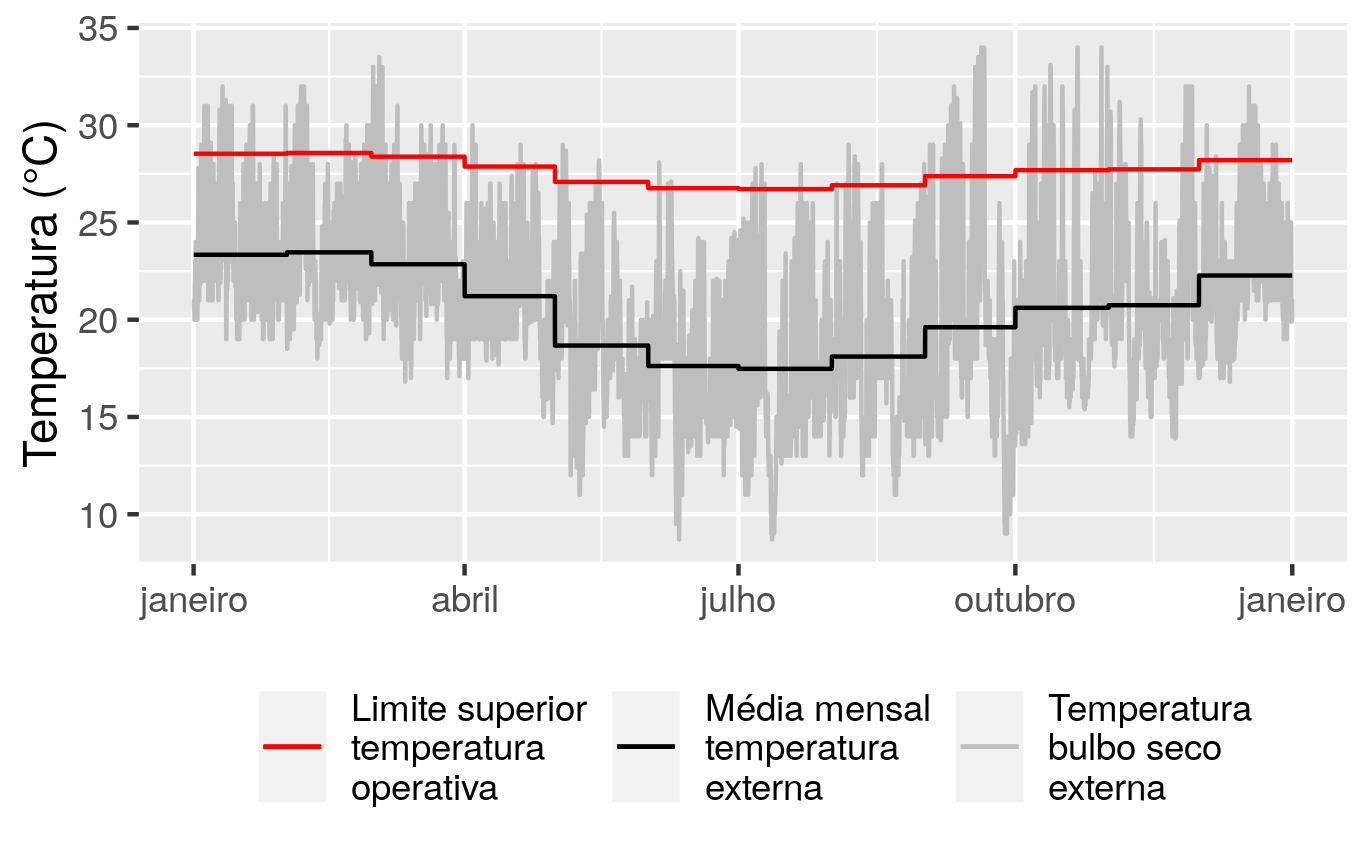
\includegraphics[width=.8\linewidth]{img/temp_means.png}
	\label{fig:temp_means}
%	\vspace{-5pt}
\end{figure}

A partir dos resultados das simulações, para cada \textit{timestep} com ocupação na sala, foi calculado se as temperaturas operativas das zonas térmicas ultrapassaram o limite superior determinado pelo método adaptativo da \citeonline{ASHRAEStandard552017}. A fração de horas de desconforto foi obtida para cada zona térmica modelada, de acordo com a Equação \ref{eq:EHF}:

\begin{equation}
\label{eq:EHF}
EHF = \frac{timesteps_{sup}}{timesteps_{ocup}}
\end{equation}

Onde:

$EHF$ é igual a fração de horas de desconforto por calor na zona térmica;

\gls{tssup} é igual ao número de \textit{timesteps} em que há ocupação na zona térmica e a temperatura operativa ultrapassa o limite superior determinado pelo método adaptativo;

\gls{tsocup} é igual ao número de \textit{timesteps} em que há ocupação na zona térmica.
\\

Para avaliar o potencial do uso de ventiladores, o movimento do ar foi considerado no desenvolvimento do metamodelo.
A \citeonline{ASHRAEStandard552017} considera um aumento no limite superior da faixa de conforto térmico de acordo com a velocidade do ar.
O aumento de aceitabilidade da temperatura operativa foi considerado para os três valores de velocidade do ar apresentados na Tabela \ref{table:var}, além da possibilidade se assumir o valor de velocidade do ar igual a zero, caso o uso de ventilador não tenha sido considerado.

\begin{table}[h]
	\centering
	\caption{Aumento no limite superior da faixa de conforto em relação à velocidade do ar}
	\label{table:var}
	\begin{tabular}{|c |c |}
		\hline
		\textbf{Velocidade média do ar} & \textbf{Temperatura} \\
		\hline
		0,6 m/s & 1,2 $^{\circ}C$ \\
		\hline
		0,9 m/s & 1,8 $^{\circ}C$ \\
		\hline
		1,2 m/s & 2,2 $^{\circ}C$ \\
		\hline 
	\end{tabular}
	\source{\citeonline{ASHRAEStandard552017}}
\end{table}

Como o modelo de \acrlong{vn} do programa EnergyPlus não calcula a velocidade do ar dentro das zonas, a consideração foi aplicada após as simulações, no momento da avaliação do conforto térmico em cada \textit{timestep}. A consideração da velocidade do ar foi realizada de acordo com a Equação \ref{eq:Tsup}.

\begin{equation}
\label{eq:Tsup}
T_{sup,v} = T_{sup} + T_{v_{ar}}
\end{equation}

Onde:

\gls{tsupv} é igual à temperatura limite superior na faixa de conforto, considerando-se a velocidade do ar ($^{\circ}C$);

\gls{tsup} é igual à temperatura limite superior na faixa de conforto definida pelo método adaptativo, sem considerar a velocidade do ar ($^{\circ}C$);

\gls{tvar} é igual à margem extra de temperatura permitida pela consideração da velocidade do ar ($^{\circ}C$).
\\

\section{Simulação termoenergética}

\subsection{Simulação detalhada}

Sabendo-se que o metamodelo estima o conforto térmico baseado no método adaptativo da \citeonline{ASHRAEStandard552017}, o principal dado de saída a se obter nas simulações foi a temperatura operativa da zona térmica, assim como a temperatura do ar externo. Portanto, todo o desenvolvimento das simulações termoenergéticas do trabalho foi voltado para que se obtivesse, com boa exatidão, a temperatura operativa das zonas térmicas e, posteriormente, a sua relação com a temperatura do ar externo, chegando-se ao indicador de conforto térmico.

%		A Tabela \ref{table:parametros} apresenta os parâmetros que serão considerados no desenvolvimento dos modelos, com suas faixas de valores admitidos.	
%		
%		\begin{table}[h]
%			\centering
%			\caption{Parâmetros considerados e variação nos valores}
%			\label{table:parametros}
%			\begin{tabular}{|l |r |}
%				\hline
%				\textbf{Parâmetro} & \textbf{Valores admitidos} \\
%				\hline
%				Área da zona & 12 - 100 [m$^2$] \\
%				\hline
%				Razão entre largura e profundidade & 0,5 - 2,0 [-] \\
%				\hline
%				Altura do pavimento & 0 - 30 [m] \\
%				\hline 
%				Azimute do eixo principal & 0 - 359 [$^{\circ}$] \\
%				\hline 
%				Pé-direito & 2,4 - 3,2 [m] \\
%				\hline 
%				Percentual de abertura da fachada & 0,1 - 0,6 [-] \\
%				\hline 
%				Fator de abertura da janela & 0,1 - 1 [-] \\
%				\hline 
%				Fator solar do vidro & 0,30 - 0,87 [-] \\
%				\hline 
%				Transmitância da parede & 0,5 - 4,7 [W/m$^2$K] \\
%				\hline 
%				Capacidade térmica da parede & 20 - 400 [kJ/m$^2$K] \\
%				\hline 
%				Absortância da parede & 0,2 - 0,9 [-] \\
%				\hline 
%				Sombreamento & 0 - 50 [$^{\circ}$] \\
%				\hline 
%				Densidade de ocupação & 0,05 - 0,50 [pessoas/m$^2$] \\
%				\hline 
%			\end{tabular}
%			\begin{flushleft}
%				Fonte: o autor.
%			\end{flushleft}				
%		\end{table}

As simulações foram realizadas através do programa de simulação computacional EnergyPlus 8.9 \cite{EnergyPlus2018} e os modelos simulados foram obtidos a partir da parametrização de uma tipologia base, que permite a variação de diferentes parâmetros.  % variados pelo método de amostragem do hipercubo latino (HCL).
A maioria desses parâmetros são numéricos e podem ser variados de forma contínua. 
Inicialmente, cada simulação representou um pavimento de uma edificação com seis salas de escritórios, onde cada sala representava uma zona térmica (Figura \ref{fig:croqui}).
O solo foi modelado pelos objetos do \textit{Ground Domain}, nos casos onde o contato com solo foi considerado. As superfícies superiores e inferiores consideradas adjacentes a outros pavimentos do edifício foram modeladas como adiabáticas.

\begin{figure}[h]
	\centering
	\caption{Croqui da tipologia base}
	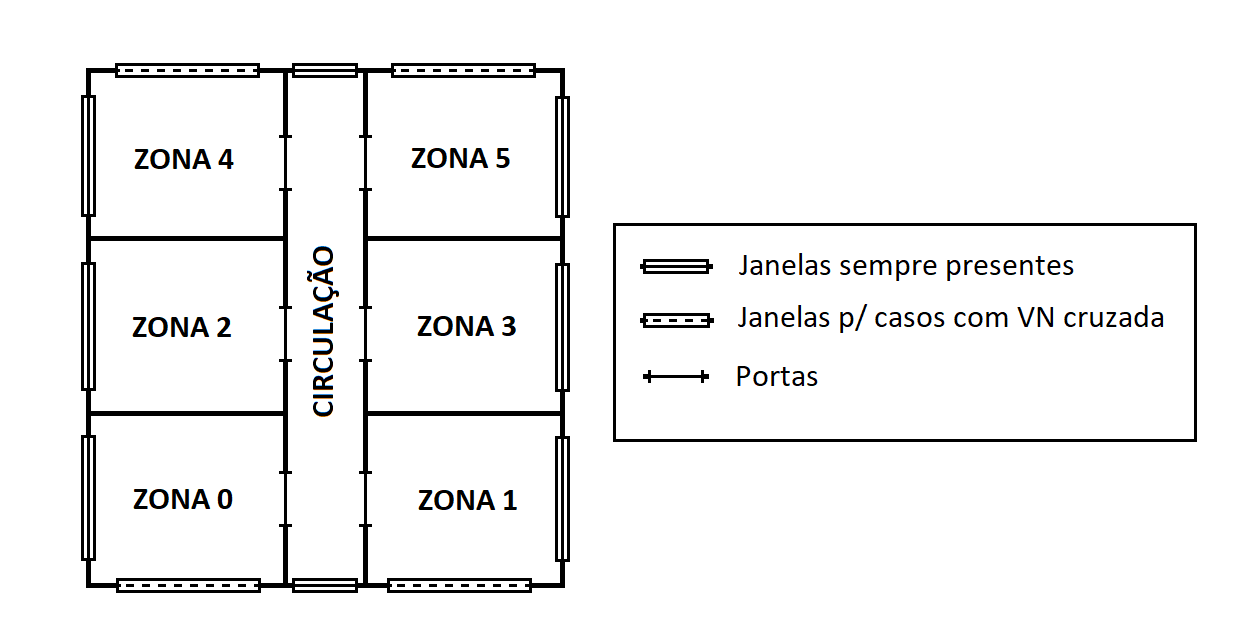
\includegraphics[width=.8\linewidth]{img/croqui_07-11.png}
	\label{fig:croqui}
\end{figure}


A partir da tipologia base, foi possível definir diferentes proporções geométricas, levando-se em consideração a largura e profundidade da edificação, assim como o pé-direito. Também foram parametrizadas a altura do pavimento e a orientação solar da edificação.
Devido a limitações na obtenção dos \acrfull{cp} para as faces externas da edificação, as edificações foram modeladas com pavimentos de forma retangular.

A parametrização nas propriedades termofísicas das paredes e vidros permitiu a consideração de diferentes materiais construtivos, possibilitando a descrição de uma quantidade significativa do universo de casos aplicáveis às edificações de escritórios consideradas. %Foram parametrizadas a transmitância térmica, capacidade térmica e absortância.

Para considerar o uso de \acrfull{vn}, é fundamental a modelagem das trocas de ar nos escritórios. A modelagem da \acrshort{vn} nas simulações foi realizada com os objetos do \acrfull{afn} do EnergyPlus \cite{EnergyPlus2018}.
Para possibilitar trocas de ar, elementos de ligação do \acrshort{afn} foram modelados em todas as zonas térmicas.
Todas as aberturas foram modeladas utilizando-se o objeto \textit{AirflowNetwork:MultiZone:Component:DetailedOpening}.
Cada sala foi modelada com uma porta, voltada para a circulação.
Na circulação, além das portas das salas, duas janelas foram modeladas, uma em cada extremidade. 
Salas com apenas uma fachada foram modeladas com uma janela; salas com duas fachadas foram modeladas com uma ou duas janelas. Isso possibilitou explorar casos com diferentes configurações de exposição das superfícies, considerando-se \acrshort{vn} unilateral e cruzada.		
As dimensões das janelas das salas foram parametrizadas de acordo com o \acrfull{paf}, permitindo diferentes frações de abertura para representar diferentes modelos de janela encontrados nas edificações de escritórios existentes no banco de dados.
%Além da área da abertura ter influência direta nas trocas de ar das zonas, a altura também pode ter influência devido à força de empuxo causada pelas diferenças de densidade do ar. Devido a isso, a altura da janela também foi parametrizada.
%		Para o vidro das janelas considerou-se diferentes valores para o fator solar.
%		\subsection{Ventilação natural no modelo preliminar}
O controle das janelas foi estabelecido pela diferença de temperatura entre o ar externo e o ar da zona.
As trocas de ar nas portas foram modeladas apenas por frestas, por considerar-se que portas de escritórios não ficam abertas normalmente.  % MELHORAR!!!
Os coeficientes de pressão nos nós externos à edificação foram definidos através da base de dados da \acrlong{tpu} \cite{TPU2018}, e para cada janela foi utilizado o valor médio dos pontos disponíveis para sua área na fachada. No o exemplo da Figura \ref{fig:tpuwindows}, considerando-se uma edificação com proporções B:L:H, e um pavimento na altura h, o \acrshort{cp} da janela A seria igual à média dos valores disponíveis para os pontos vermelhos, o \acrshort{cp} da janela B seria igual à média dos valores dos pontos verdes, e assim por diante.
%		A altura dos pontos a serem utilizadas foi escolhida de acordo com a altura definida para o pavimento simulado e  a altura do pédireito em relação às proporções do edifício.

\begin{figure}[h]
	\centering
	\caption{Exemplo de como os $C_p$ foram considerados}
	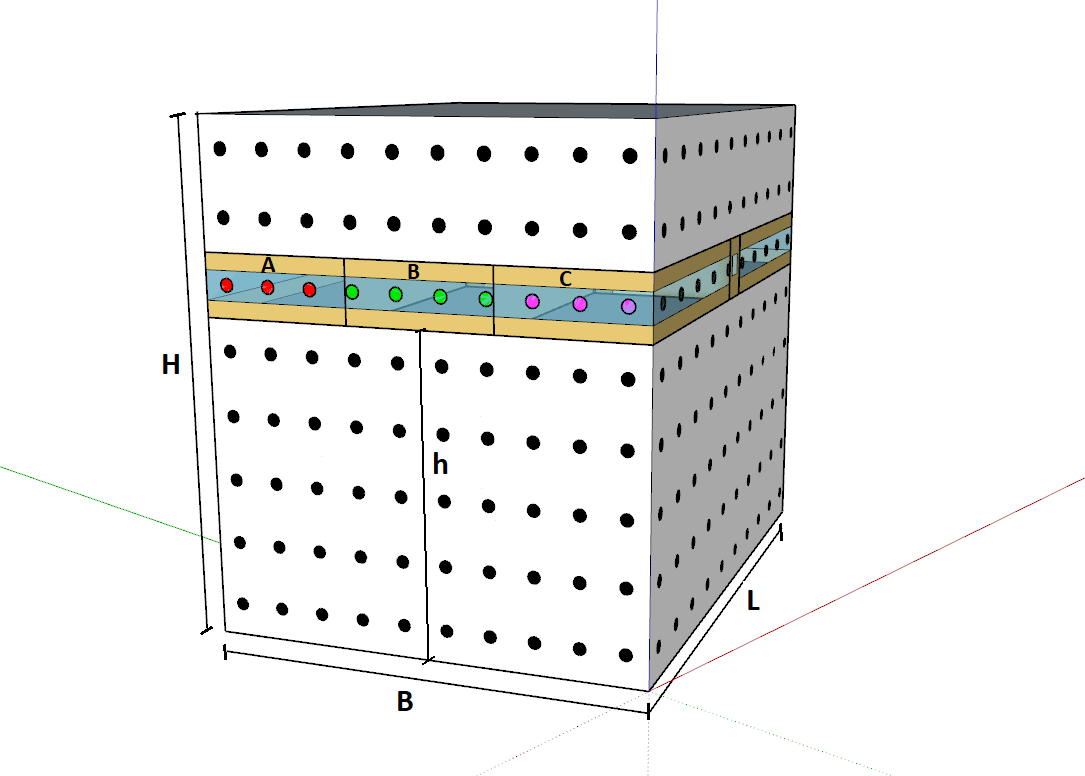
\includegraphics[width=.8\linewidth]{img/ex_TPU_h.png}
	\label{fig:tpuwindows}
\end{figure}


\subsection{Simulação simplificada}

Nesta etapa do método, buscou-se simplificar o modelo de escritório desenvolvido no EnergyPlus, atentando-se às limitações relacionadas à simplificação do modelo.
O objetivo de gerar um metamodelo por meio de \acrfull{ann} para se obter o \acrshort{ehf} faz com que se busque parametrizar ao máximo as simulações no EnergyPlus.
Essa parametrização pode facilitar o desenvolvimento de amostras para a pesquisa, assim como garantir uma relação mais direta dos parâmetros de entrada com os dados de saída. 
Dentre as simplificações consideradas, estão:

\begin{itemize}
	\item cálculo do \acrshort{cp} através do \acrlong{ma}, em vez dos valores obtidos por medições em túnel de vento pela \acrshort{tpu};
	\item representação dos materiais da envoltória através de duas camadas: uma camada representando a capacidade térmica, e uma camada para regular a transmitância;  %(concreto)  (objeto Material:NoMass)
	\item modelagem da zona que representa apenas um escritório, sem modelar as demais zonas térmicas da edificação. Para isso, são definidas as condições de contorno relacionadas às faces da zona correspondentes a paredes adjacentes à edificação;
	\item definição de um coeficiente de vazão mássica de ar relacionado à infiltração de ar pela porta, e do valor do \acrshort{cp} relacionado a essa porta, que no modelo de uma zona está voltada para o ambiente externo, e não para a circulação.
\end{itemize}

O impacto nos resultados das simulações foram verificados para cada uma das simplificações mencionadas, a partir da análise de diversos casos amostrados pelo método de amostragem do hipercubo latino (LHS). O tamanho das amostras foi definido em relação ao tempo disponível para executar as simulações.
Finalmente, foi definida a forma mais adequada de se simplificar o modelo, assim como a margem de erro que espera-se encontrar ao assumir tais simplificações.
A seguir, cada uma dessas etapas é descrita.

\subsection*{Cálculo do coeficiente de pressão pelo método analítico}

O EnergyPlus, através do \acrshort{afn}, possui uma opção para calcular automaticamente os \acrshort{cp} para as simulações.
Quando essa opção é escolhida o programa gera apenas um \acrshort{cp} por fachada da edificação, e os valores podem ser obtidos por dois algorítimos diferentes: no caso de edificações altas (\textit{highrise}), utiliza-se o modelo de \citeonline{Atkins}; no caso de edificações baixas (\textit{lowrise}), utiliza-se o modelo de \citeonline{Swami1988}.
Enquanto que pelo \acrlong{ma} os \acrshort{cp} podem ser obtidos para quaisquer razões entre as dimensões das fachadas da edificação, os valores medidos em túnel de vento pela \acrshort{tpu} são fornecidos para edificações com proporções entre largura, profundida e altura específicas.
Os valores de \acrshort{cp} para o tipo de edificação abordada neste estudo são disponibilizados pela \acrshort{tpu} para 25 geometrias diferentes, das quais 13 são para edificações \textit{highrise}, e 12 são para edificações \textit{lowrise}.

Para verificar o quanto a fonte escolhida na definição dos \acrshort{cp} influencia nos resultados das simulações, inicialmente verificou-se as diferenças entre os valores dos \acrshort{cp} das medições em túnel de vento (fornecidos pela \acrshort{tpu}), e os valores dos \acrshort{cp} obtidos pelo \acrlong{ma} (algorítimos do EnergyPlus). Para cada uma das 25 geometrias disponíveis, calculou-se a diferença entre os \acrshort{cp}, de acordo com a Equação \ref{eq:Cpdiff}. 
Geometrias definidas como \textit{highrise} pela \acrshort{tpu} foram comparadas utilizando-se o \acrlong{ma} de \citeonline{Atkins}, enquanto que geometrias definidas como \textit{lowrise} pela \acrshort{tpu} foram comparadas utilizando o \acrlong{ma} de \citeonline{Swami1988}.

\begin{equation}
\label{eq:Cpdiff}
RMSE_{Cp} = \sqrt{\frac{\sum_{i=1}^{4}{\sum_{j=0}^{11}}{\sum_{k=0}^{N_d}{(\overline{Cp}^{TPU}_{f_i,\alpha_j,p_k} - Cp^{MA}_{f_i,\alpha_j}})^2}}{48}}
\end{equation}

Onde:

\gls{rmsecp} é igual ao \acrshort{rmse} das diferenças entre os valores dos \acrshort{cp} obtidos pela base da \acrshort{tpu} e obtidos pelo \acrlong{ma};

\gls{meancptpu} é igual ao valor do \acrshort{cp} disponibilizado pela base de dados da \acrshort{tpu} para a fachada $i$ de uma edificação, para o ângulo de incidência do vento igual a $\alpha_j$, no ponto $k$;

\gls{cpma} é igual ao \acrshort{cp} calculado pelo \acrlong{ma} para a fachada de uma edificação com proporções iguais às da fachada $i$, para o ângulo de incidência do vento igual a $\alpha_j$;

\gls{fi} é a fachada $i$ da edificação avaliada;

\gls{alphaj} é o ângulo de incidência do vento  sobre a fachada, em graus, e tem valor igual a $30 \cdot j$;

\gls{nd} é o número de pontos de \acrshort{cp}` disponibilizados na fachada do edifício.	
%		$\alpha_j$ é o ângulo de incidência do vento considerado sobre a fachada, que varia de 0 a 330 graus, com intervalos de 30 graus;
\\

%		Cada \acrshort{cp} médio ($Cp_{TPU,i,j}$), medido pela \acrshort{tpu} em um ponto $j$ de uma fachada $i$, teve um \acrshort{cp} correspondente calculado pelo método analítico ($Cp_{ANALITICO, i}$), para a mesma fachada $i$. Essa subtração foi efetuada para os diferentes ângulos ($\alpha$) disponíveis na base da \acrshort{tpu}.
%		As diferenças entre os valores dos \acrshort{cp} foram calculadas obtendo-se o \acrshort{cp} pelo método analítico para cada fachada, de cada geometria disponível pela \acrshort{tpu}, e subtraindo-se o valor do \acrshort{cp} calculado pelos valores disponibilizados pela base da \acrshort{tpu} para a sua fachada correspondente (Equação \ref{eq:Cpdiff}).

A partir dessas diferenças entre os valores dos \acrshort{cp}, escolheu-se a geometria com o maior  \gls{rmsecp} como modelo base na análise da influência nos resultados das simulações no EnergyPlus.
Esta análise foi conduzida gerando-se uma amostra de 1.000 casos pelo LHS.
Os parâmetros variados e seus limites mínimos e máximos foram definidos pela metodologia do item \ref{subsec:par}, com exceção da razão entre a largura e profundidade das zonas e a altura do pavimento em relação ao solo.
A razão entre a largura e profundidade das zonas teve que ser alterada de acordo com a variação da área das salas, para se ajustar à geometria da edificação definida como modelo base da análise.
A altura do pavimento em relação ao solo também foi limitada pelas proporções da geometria escolhida para o modelo base.
Vale destacar que a base da \acrshort{tpu} permite a obtenção de diferentes \acrshort{cp} para diferentes janelas de uma mesma fachada, enquanto que nas simulações baseadas no \acrlong{ma}, utiliza-se apenas um valor de \acrshort{cp} por fachada, devido à limitação do método. 
Para cada caso da amostra gerada, foram simulados um modelo com \acrshort{cp} baseados no \acrlong{ma}, e um modelo com \acrshort{cp} baseados na base da \acrshort{tpu} (túnel de vento).
Assim, as médias anuais das \acrfull{ach} e a \acrshort{ehf} foram comparadas entre as simulações.
%		com \acrshort{cp} medidos em túnel de vento pela \acrshort{tpu}, e simulações com \acrshort{cp} obtidos pelos métodos analíticos padrão do EnergyPlus.

%		Para cada uma dessas geometrias disponíveis, valores de \acrshort{cp} são disponibilizados para diversos pontos na fachada da edificação, de acordo com a Figura \ref{fig:tpupoints}.
%		
%		\begin{figure}[h]
%			\centering
%			\caption{Exemplo do posicionamento dos pontos com valores de \acrshort{cp} na fachada}
%			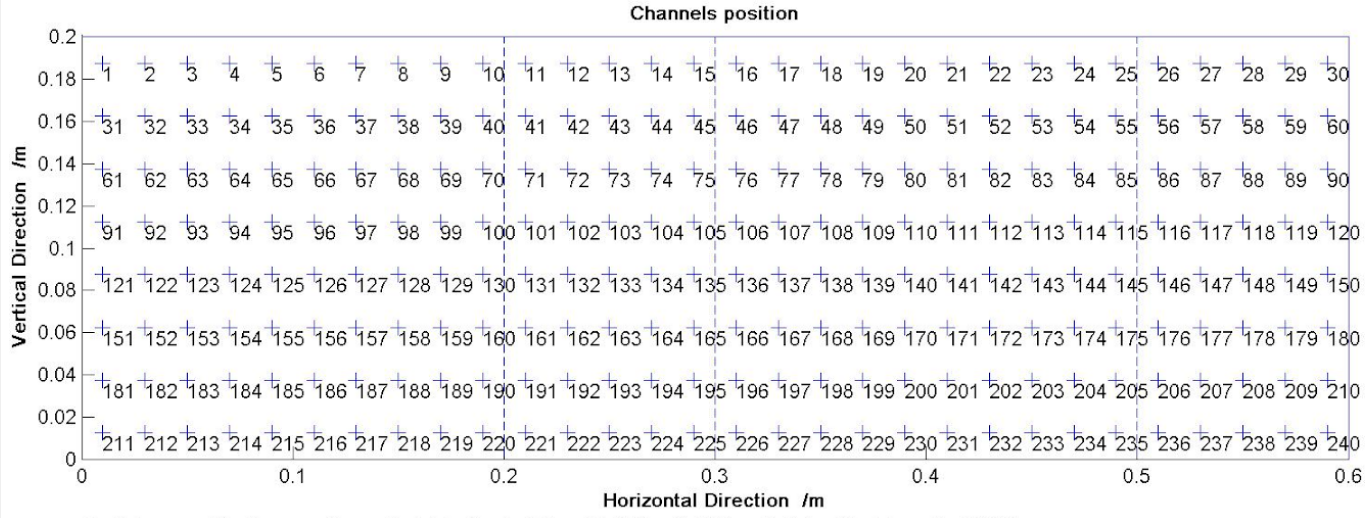
\includegraphics[width=\figsize\linewidth]{img/tpu_points.png}
%			\label{fig:tpupoints}
%			\begin{flushleft}
%				Fonte: \citeauthoronline{TPU2018} \cite{TPU2018}, adaptado pelo autor.
%			\end{flushleft}
%		\end{figure}					

\subsection*{Representação da envoltória com duas camadas}

Para possibilitar a parametrização contínua e independente das propriedades termofísicas da envoltória, considerou-se a utilização de uma parede com propriedades equivalentes, modelada com uma camada de concreto, para representar a capacidade térmica, e uma camada modelada com o objeto \textit{Material:NoMass}, para regular a transmitância (Figura \ref{fig:parede_eq}).

\begin{figure}[h]
	\centering
	\caption{Parede equivalente}
	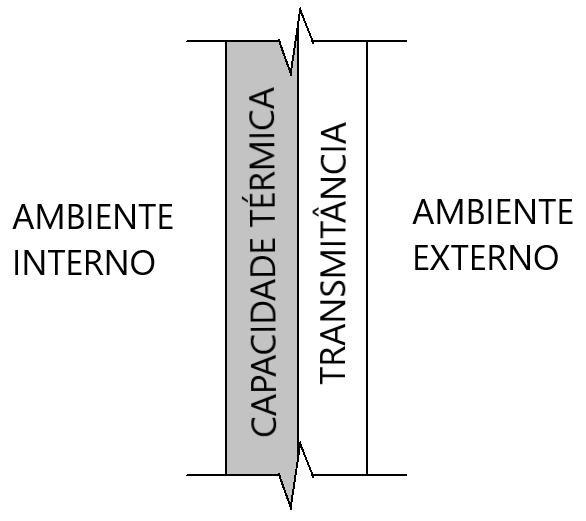
\includegraphics[width=.3\linewidth]{img/parede_eq2.png}
	\label{fig:parede_eq}
\end{figure}

A validação da modelagem simplificada da parede foi realizada para dois tipos de paredes referência (uma leve, outra pesada):

\begin{itemize}
	%			\item parede de concreto;
	\item parede de gesso com lã de rocha (leve);
	\item parede de alvenaria e reboco (pesada).
\end{itemize}

Como a modelagem da parede de alvenaria possui uma camada de ar no meio da parede, avaliou-se a possibilidade de considerar apenas a metade interna desta parede referência para definir a capacidade térmica de sua parede equivalente. Essa consideração parte do pressuposto de que a camada interna de ar faz com que a inércia térmica da metade exterior da parede não influencie consideravelmente a zona térmica analisada.

Para validar essa simplificação, gerou-se uma amostra utilizando LHS, com 100 casos.
Os parâmetros variados e seus limites mínimos e máximos foram definidos pela metodologia do item \ref{subsec:par}, com exceção da transmitância e capacidade térmica da parede.  % os parâmetros relacionados com a propriedades termofísicas da parede.	% e a absortância????
%		O modelo preliminar sofreu variação dos seguintes parâmetros: área, razão entre largura e profundidade da zona, pé-direito, azimute, absortância, \acrshort{paf}, taxa de ocupação. Os demais parâmtros foram fixados de acordo com a Tabela \ref{table:paramfix}.
Cada caso da amostra foi simulado com os dois tipos de paredes diferentes, e suas paredes equivalentes. No caso da parede de alvenaria, dois modelos de parede equivalente foram desenvolvidos: considerando o valor total da capacidade térmica da parede, e considerado apenas metade do valor da capacidade térmica.
A partir dos resultados, observou-se a diferença média entre as temperaturas operativas das zonas simuladas com as paredes referências em relação às simulações com as respectivas paredes equivalentes. O mesmo foi realizado comparando-se o \acrshort{ehf}.

\subsection*{Condição de contorno das paredes adjacentes à edificação}

Simular apenas uma zona térmica, em vez de um edifício inteiro, ou um pavimento com diversas zonas, possibilita a simulação de casos diversos em menor tempo.
Essa consideração facilita a parametrização do modelo, e pode oferecer resultados satisfatórios se for adequadamente implementada.
A partir dessa premissa, foi desenvolvido um modelo com apenas uma zona térmica (Figura \ref{fig:singlezone}).

\begin{figure}[h]
	\centering
	\caption{Modelo de uma zona}
	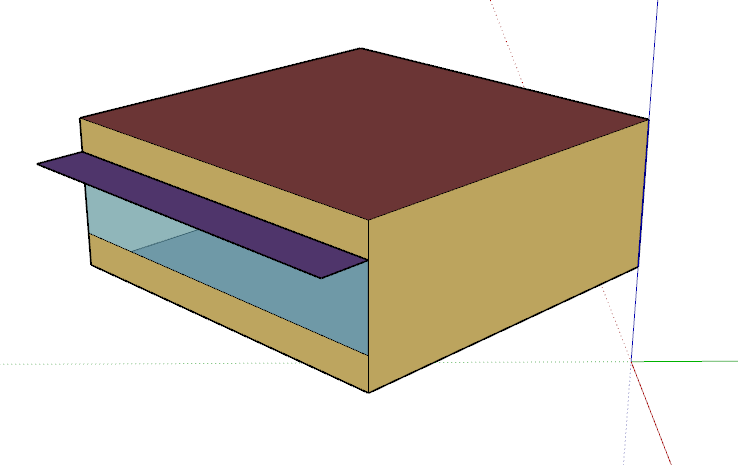
\includegraphics[width=\figsize\linewidth]{img/model.PNG}
	\label{fig:singlezone}
\end{figure}

Para modelar essa zona, considerou-se as paredes correspondentes a superfícies voltadas para outros escritórios como adiabáticas (sem trocas de calor). A superfície que representa a parede voltada para a circulação foi avaliada com duas condições de contorno: 1) como adiabática, e 2) como \textit{outdoors}, sem incidência de vento ou sol (Figura \ref{fig:adiabatic_outdoors}).	
A consideração do uso da condição \textit{outdoors} foi realizado pela hipótese de que, sem a radiação solar direta e sem o aumento de convecção causada pelo vento, a temperatura do ar da zona da circulação (por não ter cargas internas consideráveis) poderia se manter mais próxima à temperatura do ar externo do que às das zonas das salas de escritórios.

\begin{figure}[h]
	\centering
	\caption{Modelagem com parede adiabática e \textit{outdoors}}
	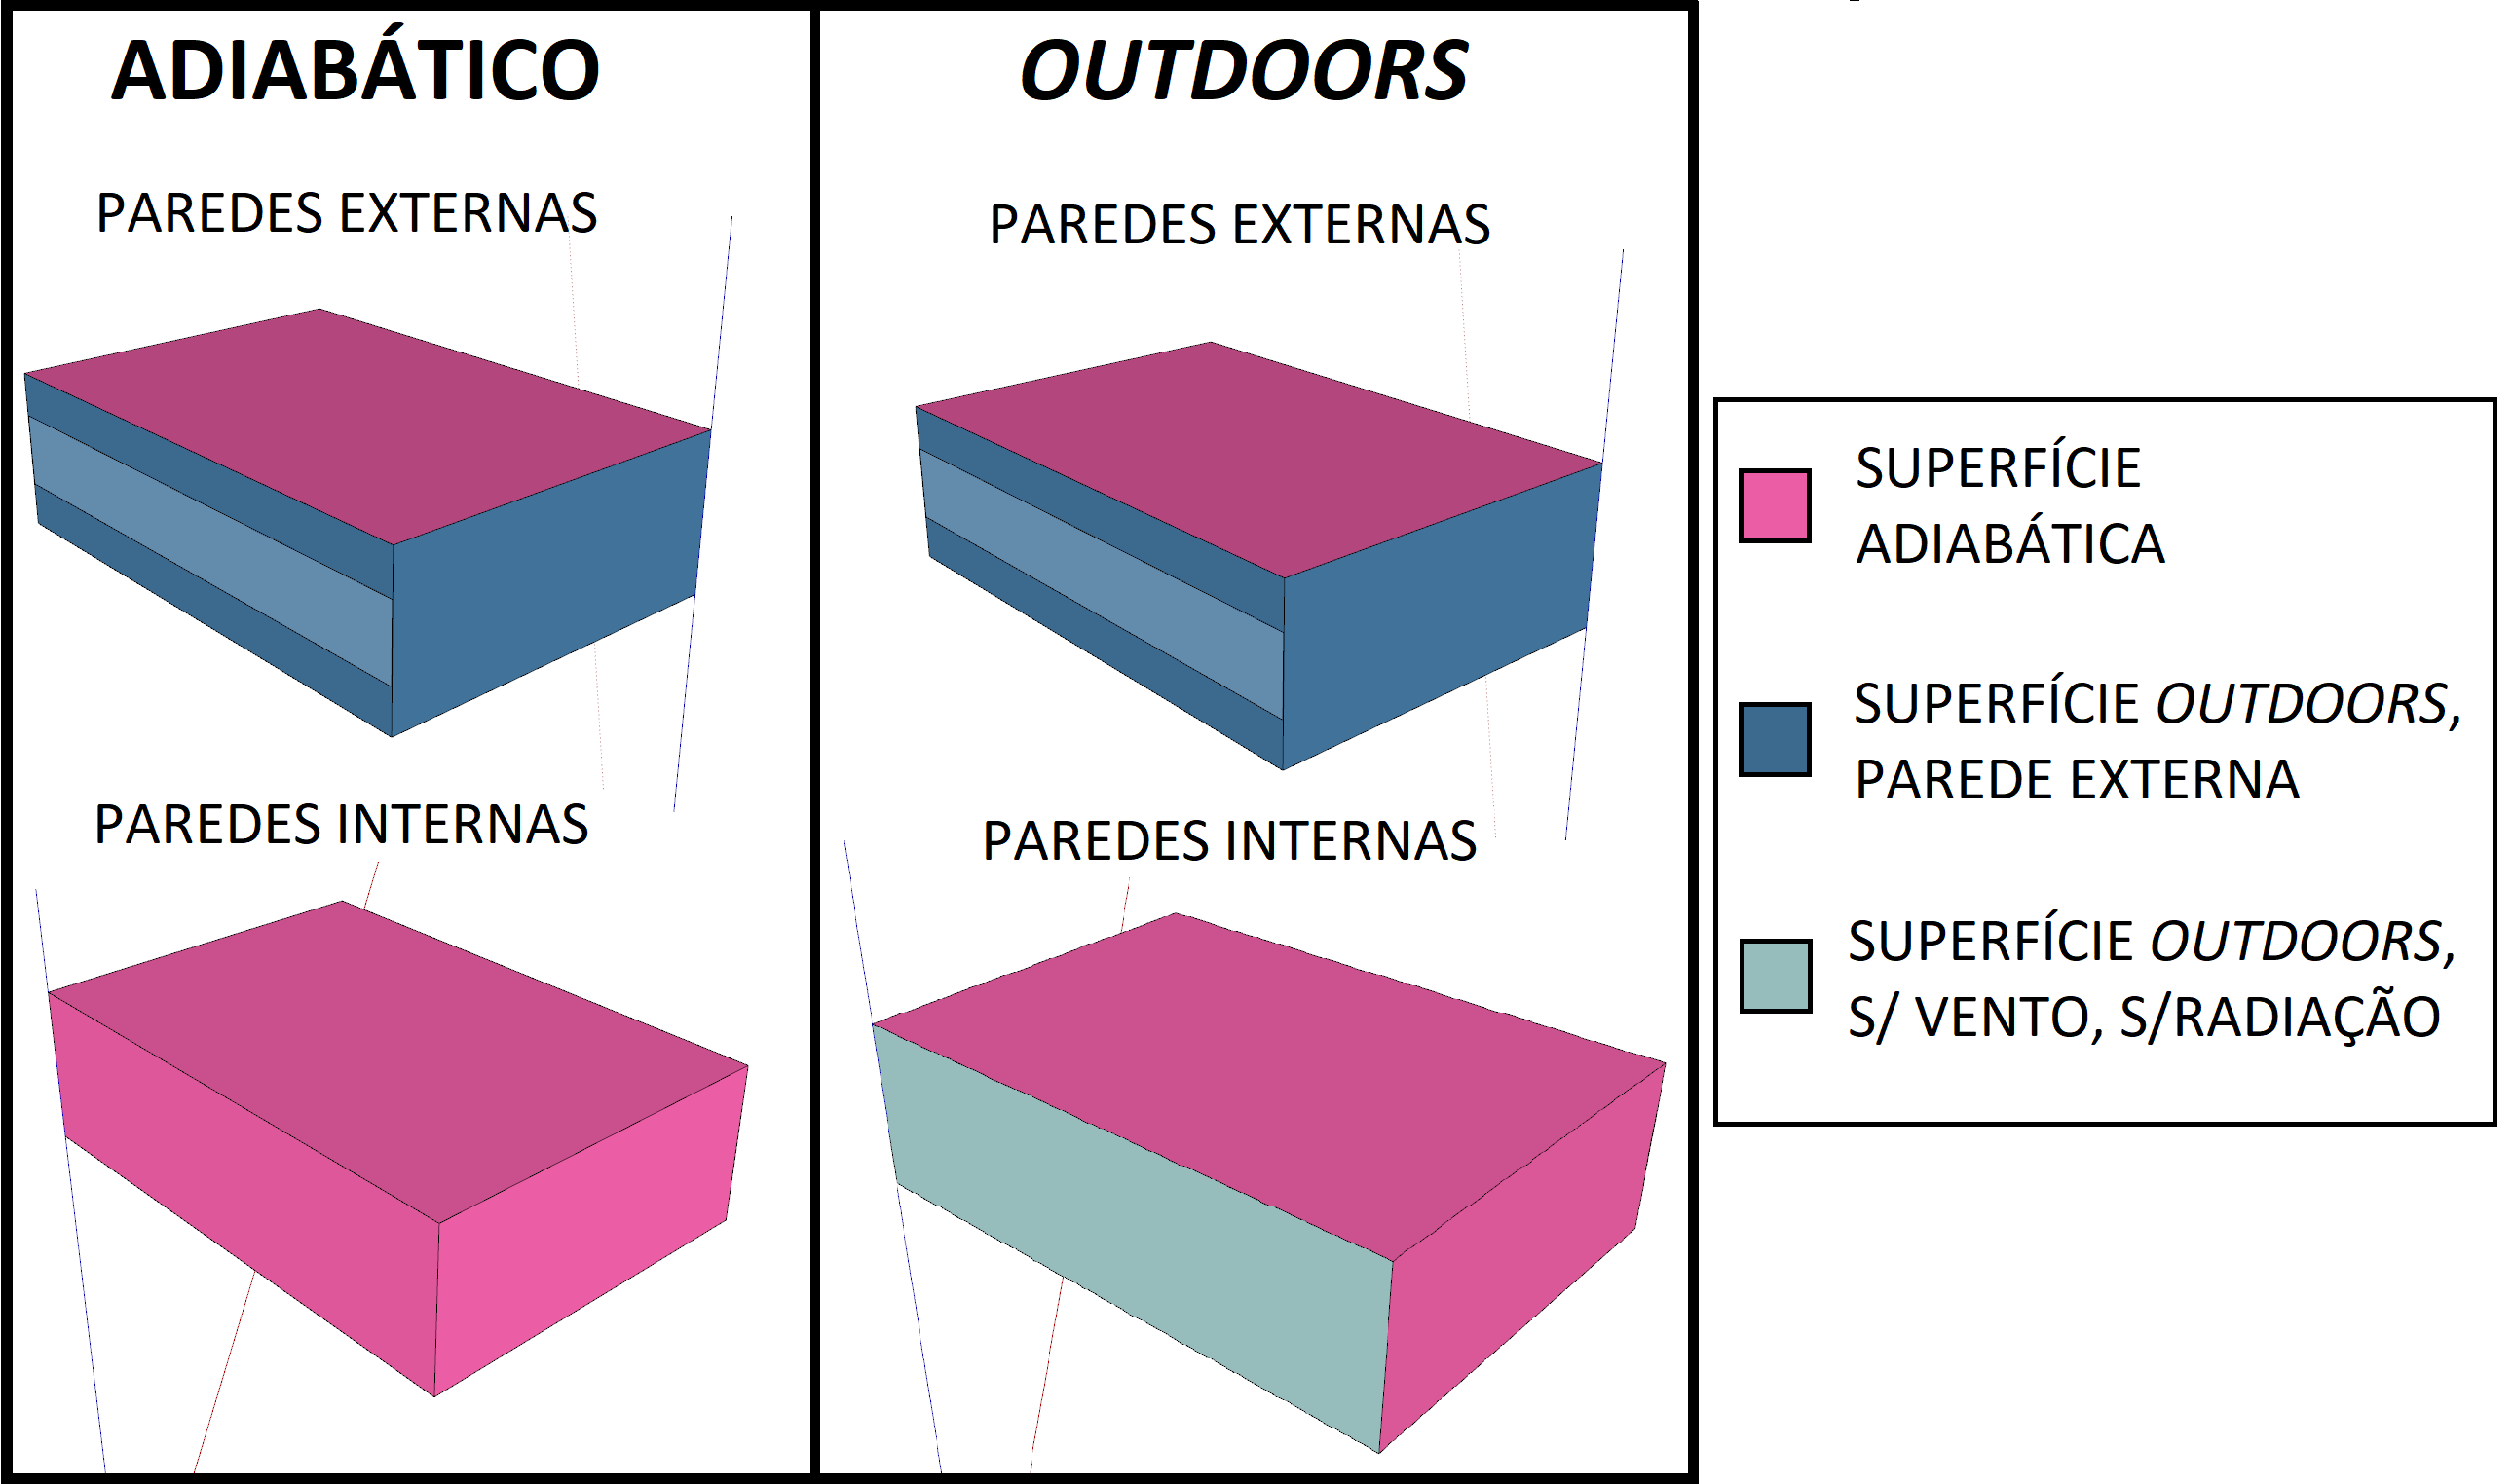
\includegraphics[width=.7\linewidth]{img/adiabatic_outdoors2.png}
	\label{fig:adiabatic_outdoors}
\end{figure}


A modelagem da \acrlong{vn} sofre um impacto significativo quando o escritório é modelado como apenas uma zona térmica.
Esse impacto é devido à forma como a rede de fluxo de ar é distribuída. No caso do modelo detalhado, a porta é voltada para a circulação, enquanto que no caso de uma única zona térmica, a porta desta zona é voltada para o ambiente externo. 
Além disso, não é possível modelar uma porta em uma parede adiabática. Para não deixar a diferença na \acrlong{vn} influenciar as análises comparativas entre as simulações, a \acrlong{vn} não foi modelada para esta etapa.
Em vez disso, as simulações foram desenvolvidas com uma taxa de infiltração de ar constante durante a ocupação. O valor escolhido para a taxa de renovação de ar foi igual ao valor médio do \acrshort{ach} obtido na etapa da comparação entre os \acrshort{cp}, que é igual a 30 \acrshort{ach}.

A amostra gerada pelo LHS nesta etapa foi de 100 casos.
Os parâmetros variados e seus limites mínimos e máximos foram definidos pela metodologia do item \ref{subsec:par}.
Para cada caso gerado pelo LHS, além da simulação detalhada, seis modelos de uma zona foram simulados, correspondendo a cada uma das zonas do modelo detalhado.
Para validar o uso de diferentes condições de contorno, comparou-se os resultados de \acrshort{ehf} e temperaturas operativas das simulações de uma zona térmica com os resultados obtidos para as zonas térmicas das simulações detalhadas.
A condição de contorno com menores diferenças médias, de temperatura operativa e \acrshort{ehf}, foi escolhida para se conduzir as simulações simplificadas.

\subsection*{Modelagem da ventilação natural na simulação simplificada}

A modelagem da \acrlong{vn} na simulação simplificada deve ser adaptada para se ter resultados correspondentes ao esperado em relação à simulação detalhada, pois enquanto a rede de fluxo de ar na simulação detalhada é modelada de acordo com a Figura \ref{fig:AFN_ref}, na simulação simplificada essa rede é modelada de acordo com a Figura \ref{fig:AFN_sz}.	

\vspace{20pt}
\begin{figure}[h]
	\centering
	\caption{Rede de fluxo de ar na simulação detalhada}
	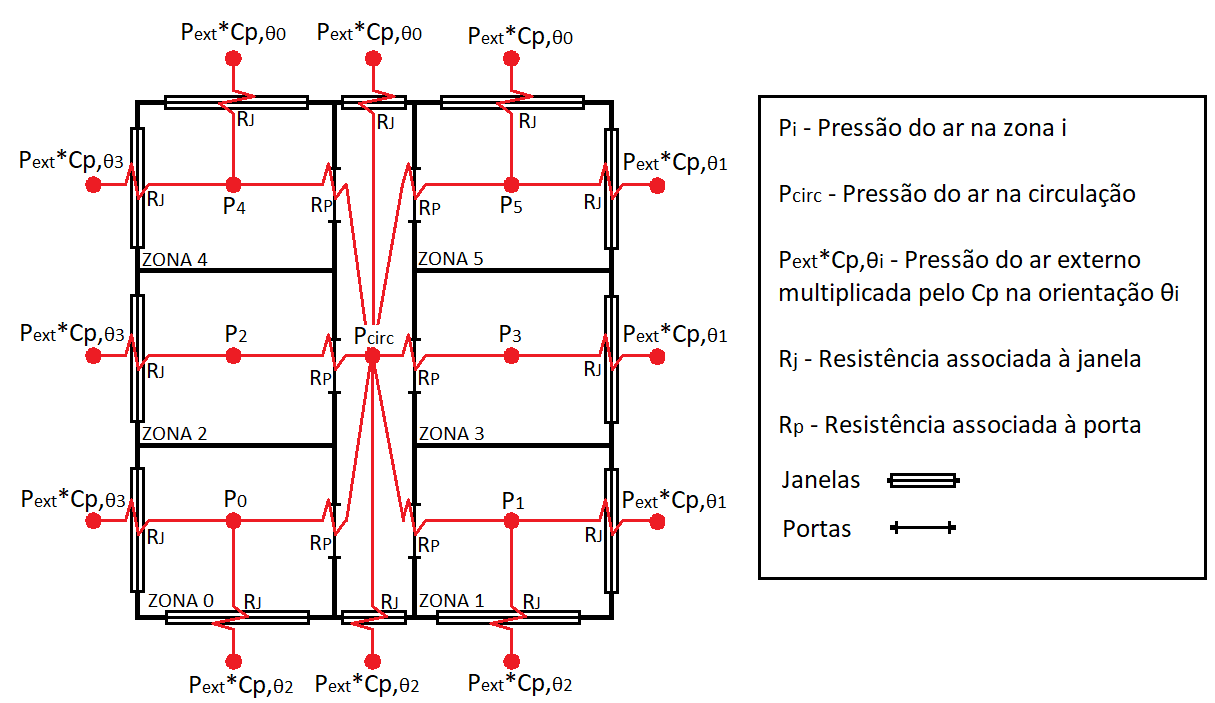
\includegraphics[width=1\linewidth]{img/AFN_ref2.png}
	\label{fig:AFN_ref}
\end{figure}	

\begin{figure}[h]
	\centering
	\caption{Rede de fluxo de ar na simulação simplificada}
	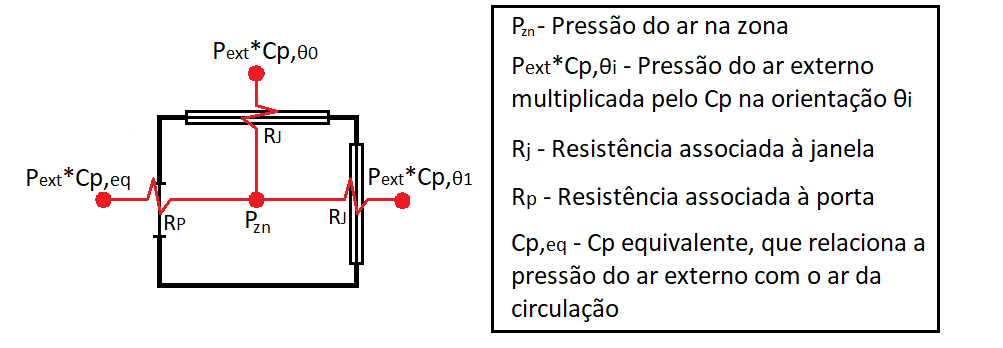
\includegraphics[width=.8\linewidth]{img/AFN_sz2.png}
	\label{fig:AFN_sz}
\end{figure}
\newpage
A proposta para contornar esse problema foi desenvolvida a partir da hipótese de que, na simulação simplificada, seria possível criar um \acrshort{cp} associado à porta ($Cp_{eq}$), capaz de descrever as diferenças de pressão de ar entre a circulação e a sala.  % , para cada ângulo de vento.

Quando o objeto \textit{AirflowNetwork:MultiZone:Component: DetailedOpening} é utilizado, o cálculo do fluxo de ar entre dois pontos é feito pela Equação \ref{eq:AFEDOP_opened}, se a porta/janela está aberta, ou pela Equação \ref{eq:AFEDOP_closed}, que é utilizada para calcular a infiltração de ar quando a abertura está fechada.

\begin{equation}
\label{eq:AFEDOP_opened}
\dot{m}_{i,j} = C_d \Theta 	\int_{z=0}^{z=H} \sqrt{2 \rho (P_{i(z)} - P_{j(z)})} W d_z 
\end{equation}

\begin{equation}
\label{eq:AFEDOP_closed}
\begin{split}
\dot{n}_{i,j} = C_Q [2\int_{z=0}^{z=H} {(P_{i(z)} - P_{j(z)})}^{exp} d_z + \\ W{(P_{i(0)} - P_{j(0)})}^{exp} + W{(P_{i(H)} - P_{j(H)})}^{exp}]
\end{split}
\end{equation}

Onde:

\gls{m} é o fluxo de ar entre os pontos $i$ e $j$, quando a porta/janela está aberta (kg/s);

\gls{cdd} é o coeficiente de descarga da abertura ($-$);

\gls{theta} é a fração de abertura ($-$);

\gls{height} é a altura da abertura ($m$);

\gls{piz} é a pressão de ar no ponto $i$, altura $z$ ($Pa$);

\gls{width} é a largura da abertura ($m$);

\gls{n} é o fluxo de ar entre os pontos $i$ e $j$, quando a porta/janela está fechada ($kg/s$);

\gls{cqq} é o coeficiente de vazão mássica de ar da abertura ($-$);

\gls{exp} é o expoente de vazão mássica de ar ($-$).
\\

As seguintes condições de contorno foram estabelecidas para facilitar o cálculo do $Cp_{eq}$:
\begin{itemize}			 
	\item o valor do $exp$ foi definido como 0,5;
	\item o valor de $\rho$ foi definido sempre como 1,200 kg/m$^3$;
	\item os fluxos de ar foram considerados como unidimensionais, portanto os valores de $P$ não variaram com o a altura ($z$);
	\item O valor do $Cp_{eq}$ foi definido assumindo-se que as janelas estariam com sua máxima fração de abertura ($\Theta$).
\end{itemize}

Em cada \textit{timestep}, a soma dos fluxos de ar que entram e saem de uma zona $i$ é igual a zero. Assumindo-se as condições de contorno descritas, a pressão de ar em cada zona térmica pode ser estimada pela Equação \ref{eq:P}. Dessa forma é possível encontrar a relação entre as pressões de ar de todas as zonas da simulação detalhada.

\begin{equation}\label{eq:P}
%\resizebox{\linewidth}{!}{
\begin{split}
P_{zn} = \frac{\sum_{i=1}^{N_P}{P_{i} (C_q L_i)^2} +  %\\
	\sum_{j=1}^{N_J}{(P_{d} C_{p,j} + P_{\infty}) 2 \rho (C_{d} \Theta_j A_j)^2 }}
{\sum_{i=1}^{N_P}{(C_q L_i)^2} +  %\\
	\sum_{j=1}^{N_J}{2 \rho (C_{d} \Theta_j A_j)^2 }}
\end{split}
%}
\end{equation}

Onde:

\gls{pzn} é a pressão do ar na zona analisada ($Pa$);

\gls{np} é igual ao número de portas que se conectam à zona ($-$);

\gls{pi} é a pressão de ar na zona ligada pela porta $i$ ($Pa$);

\gls{li} é igual ao perímetro da porta $i$ ($m$);

\gls{nj} é igual ao número de janelas que se conectam à zona ($-$);

\gls{pd} é a pressão dinâmica do ar ($Pa$);

\gls{p0} é a pressão estática do ar no ambiente externo ($Pa$);

\gls{cpj} é o \acrshort{cp} na superfície da janela $j$ ($-$);

\gls{area} é igual à área da janela $j$ ($m^2$).
\\

Finalmente, os \acrshort{cp} equivalentes (\acrshort{cpeq}) foram definidos calculando-se a relação entre a pressão de ar na zona da circulação e a pressão do ar no ambiente externo, para cada direção angular do vento, de acordo com a Equação \ref{eq:Cpeq}.

\begin{equation}\label{eq:Cpeq}
Cp_{eq,\alpha} = \frac{P_{circ}-P_{\infty}}{P_{d}}
\end{equation}

Onde:

$P_{circ}$ é a pressão de ar na circulação;

$Cp_{eq,\alpha}$ é igual ao \acrshort{cp} equivalente na abertura da porta, para um ângulo de vento $\alpha$.
\\

Outra limitação relacionada à \acrshort{vn} na simulação simplificada é o fato de que o \acrshort{afn} do EnergyPlus não permite modelar aberturas ou qualquer tipo de infiltração de ar em superfícies adiabáticas. Para contornar esse problema, no caso de se modelar uma parede voltada para a circulação como adiabática, é possível associar a infiltração referente à porta a uma outra superfície da zona.  %  que esteja voltada para o ambiente externo 
Isso se faz possível no momento em que se calcula diretamente os \acrfull{cp} dos nós relacionados às aberturas da zona térmica.
Desta forma define-se o \acrshort{cp} para uma superfície (seja janela ou parede), considerando-se qualquer orientação desejada, e não necessariamente a orientação definida para esta superfície pela geometria do modelo.		
A modelagem do fluxo de ar pelas portas dos escritórios nas simulações simplificadas foi desenvolvida com o objeto \textit{AirflowNetwork:MultiZone:Surface:Crack}. O motivo para se utilizar este objeto é porque este é um objeto que pode ser associado a qualquer tipo de superfície. Portanto, o objeto do \textit{crack} foi associado sempre à parede externa oposta à parede que estaria voltada para a circulação, como apresentado na Figura \ref{fig:AFN_crack}.

Devido a essas considerações, a validação nesta etapa foi conduzida para duas condições: utilizando-se o \acrshort{cp} calculado diretamente pelo método analítico, e utilizando-se o \acrfull{cpeq}.		
Estas análises foram conduzidas considerando-se diferentes valores de coeficiente de vazão mássica de ar para o \textit{crack}, para ajustar o valor mais adequado à taxa de infiltração que se obtém no modelo detalhado. Os valores considerados foram: 0,10; 0,30; 0,40; 0,45; 0,50; 0,55; 0,6; 0,7; 0,80; e 0,90 kg/s em 1 Pa.
Uma amostra de 200 casos foi gerada por LHS.
Os parâmetros variados e seus limites mínimos e máximos foram definidos pela metodologia do item \ref{subsec:par}.
Para cada caso, gerou-se uma simulação detalhada, mais 120 simulações simplificadas. Essas 120 simulações simplificadas devem-se à consideração dos dois métodos para se obter os \acrshort{cp}, mais os dez valores de coeficiente de vazão mássica de ar analisados, avaliados para as seis zonas térmicas do modelo detalhado. 
Para escolher a configuração mais adequada entre os métodos de obtenção do \acrshort{cp} e o coeficiente de vazão mássica de ar, as comparações foram efetuadas observando-se os resultados das médias anuais de \acrshort{ach} e \acrshort{ehf}.
A escolha da melhor configuração observando-se dois indicadores simultaneamente foi possível através de uma análise de eficiência de Pareto.
%Como as taxas de infiltração são influenciadas pela temperatura do ar, as comparações com os modelos detalhados foram feitas considerando-se diferentes faixas de temperatura.

\begin{figure}[H]
	\centering
	\caption{Solução para infiltração de ar entre a zona e a circulação}
	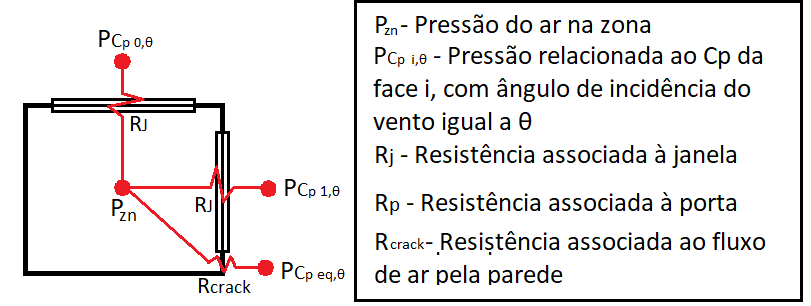
\includegraphics[width=.8\linewidth]{img/AFN_crack2.png}
	\label{fig:AFN_crack}
\end{figure}
%\vspace{-100pt}

\section{Análise de sensibilidade}

Após definir como seriam desenvolvidos os modelos para as simulações simplificadas, uma \acrfull{as} foi aplicada. Através da \acrshort{as}, a influência dos diferentes dados de entrada variados nas simulações foi avaliada. Com base nos resultados da \acrshort{as}, parâmetros não relevantes nos resultados de temperatura operativa e, consequentemente, \acrfull{ehf}, foram determinados com valores fixos. Desta forma, o metamodelo foi desenvolvido considerando-se apenas parâmetros com influência expressiva nos dados de saída desejados.

O método de \citeauthoronline{Sobol1993} \cite{Sobol1993} foi utilizado para a \acrshort{as}, pois permite a identificação de parâmetros influentes, mesmo para casos onde a relação entre as entradas e saídas dos modelos são não-monotônicas e apresentam efeitos colineares.

A \acrshort{as} foi aplicada por meio de programação, utilizando-se a biblioteca \textit{SALib} \cite{Herman2017}, escrita na linguagem \citeonline{Python}, versão 3.
Os casos simulados para conduzir a \acrshort{as} foram amostrados pelo método de amostragem específico da \acrshort{as} de Sobol, pelo qual gerou-se uma amostra de 155.648 casos.
Os parâmetros variados e seus limites mínimos e máximos foram definidos pela metodologia do item \ref{subsec:par}. 
%, que gera uma sequência quasi-randômica de baixa discrepância.é uma é feita a partir de uma amostra desenevolvida específica para essa análise é definida pelo próprio método, pela qual gerou-se 99.978 casos.		
A partir dos dados de entrada de cada caso, e dos valores das médias anuais de \acrshort{ach}, médias anuais de temperatura operativa, e \acrshort{ehf} resultantes das simulações termoenergéticas, obteve-se índices de sensibilidade para análise de primeira ordem, segunda ordem, e efeitos totais.
%\vspace{50pt}
\newpage

\section{Desenvolvimento do metamodelo}

O metamodelo foi desenvolvido por meio de \acrfull{ann}, utilizando a biblioteca \textit{TensorFlow} \cite{tensorflow2015}, disponibilizada para \citeonline{Python}.
A maneira como se descreve as variáveis de entrada dos modelos simulados para o metamodelo a ser desenvolvido pode influenciar na sua precisão e na representação adequada dos fenômenos termofísicos.
Portanto, no processo de definição das variáveis de entrada do metamodelo, busca-se a melhor forma de descrever as diversas características das zonas térmicas.
Esse é um processo iterativo, que envolve diferentes variáveis, utilizando-se transformações, normalizações e funções destas. 
É importante também observar os hiperparâmetros (parâmetros relacionados ao processo de aprendizagem automática) escolhidos no desenvolvimento da \acrshort{ann}. 
A exatidão dos resultados obtidos pela \acrshort{ann} pode depender do número de nós, número de camadas, taxa de aprendizagem, número de iterações, assim como outros parâmetros definidos durante o processo de treinamento. 

Ao longo do processo de desenvolvimento do metamodelo, \acrshort{ann} com diferentes configurações foram testadas, utilizando-se diferentes maneiras de descrever as variáveis de entrada, e diferentes combinações de hiperparâmetros.
A base de dados utilizada para o treinamento do metamodelo foi gerada a partir de 100.000 simulações, amostrados pelo método de amostragem do LHS. %100.000 simulações, amostrados pelo método de amostragem de Sobol.
A amostra utilizada para validação foi composta por 20.000 casos, geradas por LHS.
% O motivo para se utilizar diferentes métodos de amostragem é para evitar qualquer enviesamento possivelmente relacionado ao método de amostragem.
Em ambas as amostras, os parâmetros variados tiveram seus limites mínimos e máximos definidos de acordo com o item \ref{subsec:par}, com excessão daqueles parâmetros que tiveram seus valores determinados como fixos na etapa da \acrshort{as}.
Os indicadores de exatidão utilizados foram o erro absoluto médio e o \acrfull{ae95}.
É comum se utilizar a \acrfull{rmse}, ou o \acrfull{r2} como indicadores de desempenho. Contudo, considerando-se que o dado de saída do metamodelo será uma fração (\acrshort{ehf}) com valor entre zero e um, o erro absoluto já é consequentemente um erro relativo. Portanto, conclui-se que o erro absoluto médio, associado ao \acrlong{ae95}, pode estimar de maneira mais adequada a exatidão esperada para os resultados do metamodelo.

A \acrshort{ann} com os melhores indicadores de exatidão na etapa de treinamento foi escolhida para ter seu desempenho analisado com uma amostra de teste. 
A amostra de teste foi utilizada para verificar o desempenho da \acrshort{ann} quando os valores dos parâmetros determinados como fixos na etapa da \acrshort{as} variam. Para isso, utilizou-se uma amostra de 20.000 casos.
Ao analisar os indicadores de exatidão da \acrshort{ann} em relação às amostras de validação e de teste, o metamodelo final foi definido.

\chapter{Resultados e discussões}
\label{chapter:Resultados}

\section{Parâmetros de entrada} \label{section:parametrosdeentrada}
Ao analisar o banco de dados disponibilizado por \citeonline{Neves2019}, obteve-se as distribuições de ocorrência em relação aos parâmetros observados (Figura \ref{fig:db_hist}).

\begin{figure}[H]
	\captionof{figure}{Distribuições de ocorrência}
	\label{fig:db_hist}
	\centering
	\begin{minipage}{.33\textwidth}
		\centering
		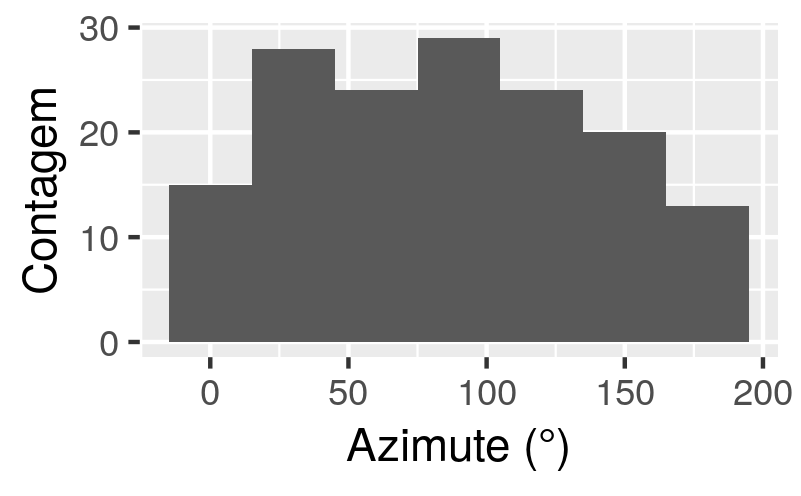
\includegraphics[width=\linewidth]{img/hist_azimute.png}
	\end{minipage}%
	\begin{minipage}{.33\textwidth}
		\centering
		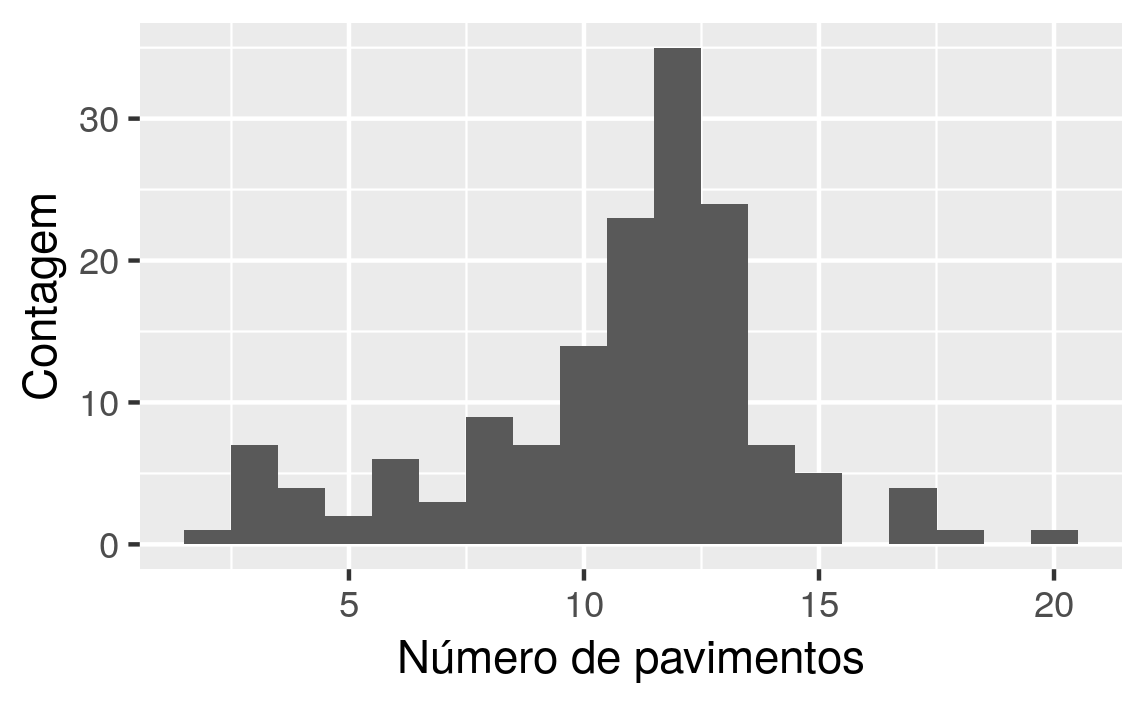
\includegraphics[width=\linewidth]{img/hist_numero_pavimentos.png}
	\end{minipage}%
	\begin{minipage}{.33\textwidth}
		\centering
		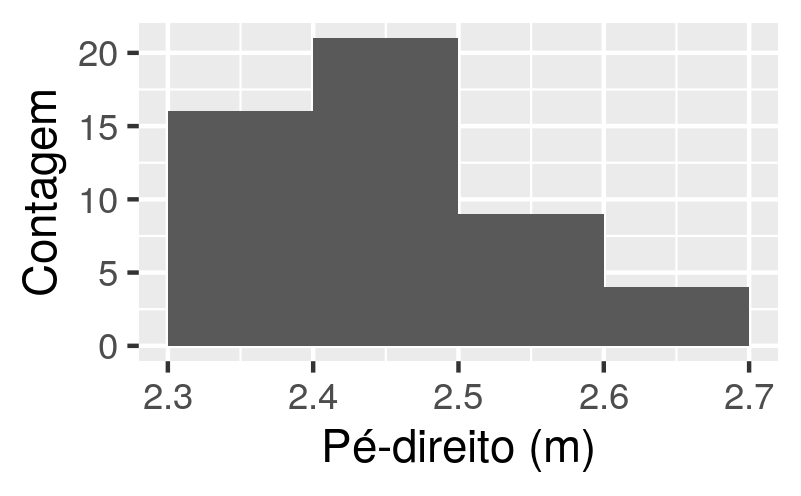
\includegraphics[width=\linewidth]{img/hist_pe_direito.png}
	\end{minipage}
	\centering
	\begin{minipage}{.33\textwidth}
		\centering
		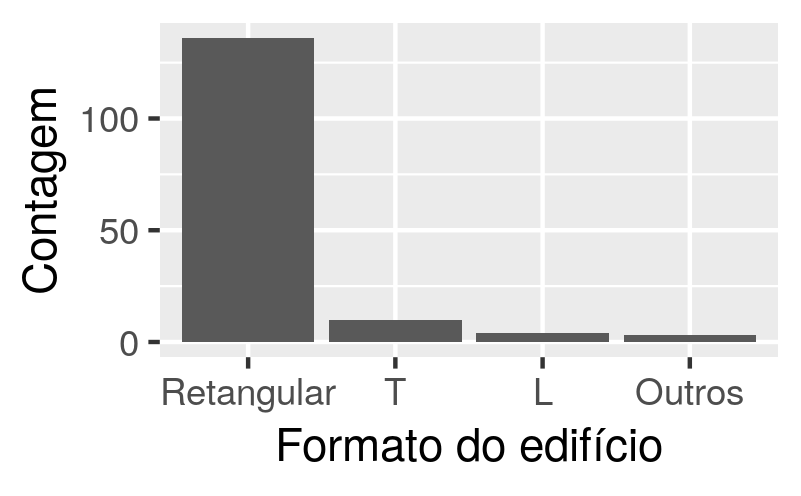
\includegraphics[width=\linewidth]{img/hist_formato.png}
	\end{minipage}%
	\begin{minipage}{.33\textwidth}
		\centering
		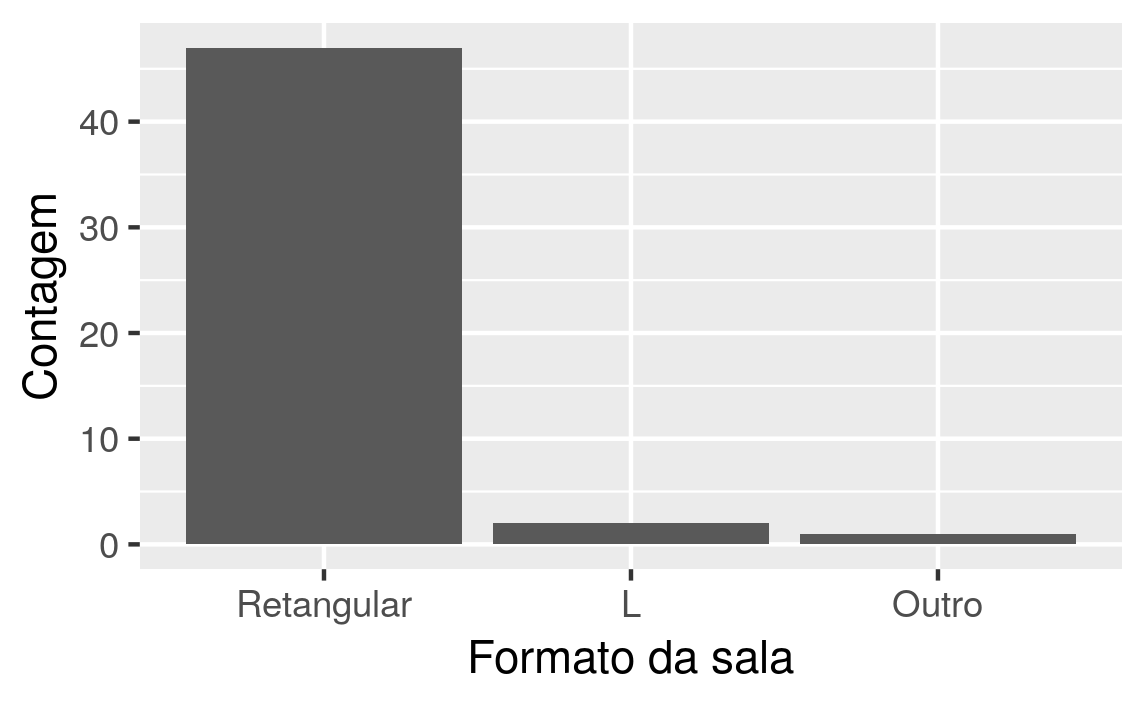
\includegraphics[width=\linewidth]{img/hist_formato_sala.png}
	\end{minipage}%
	\begin{minipage}{.33\textwidth}
		\centering
		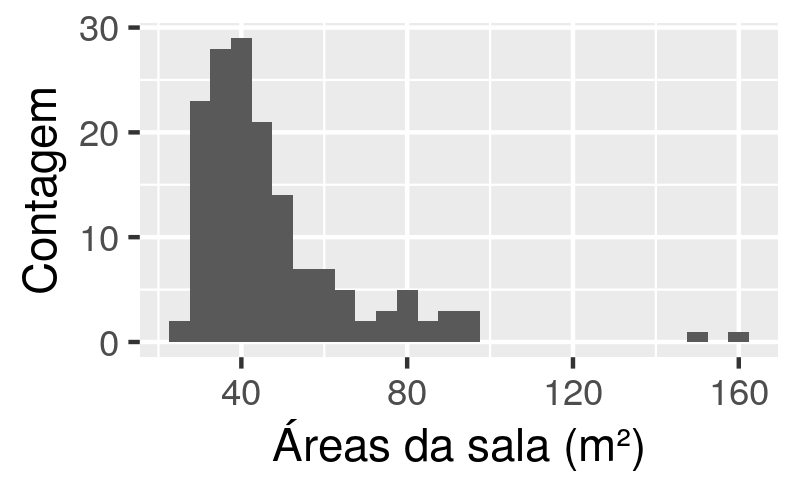
\includegraphics[width=\linewidth]{img/hist_area_zonas.png}
	\end{minipage}
	\centering
	\begin{minipage}{.33\textwidth}
		\centering
		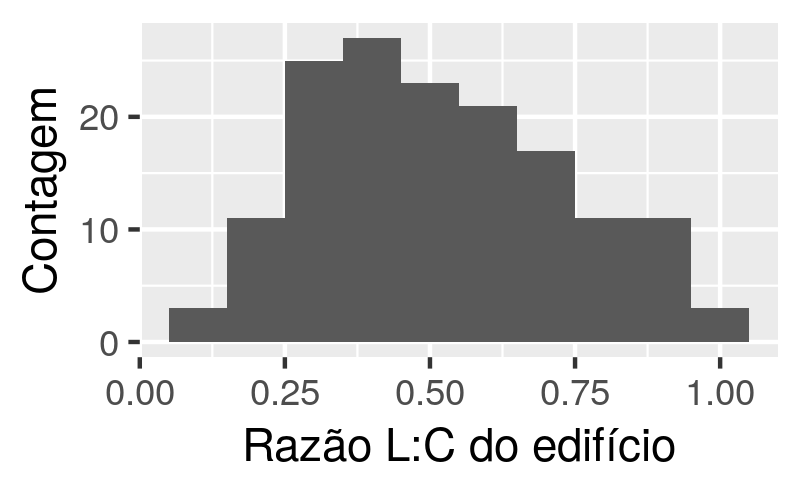
\includegraphics[width=\linewidth]{img/hist_ratio_edificio.png}
	\end{minipage}%
	\begin{minipage}{.33\textwidth}
		\centering
		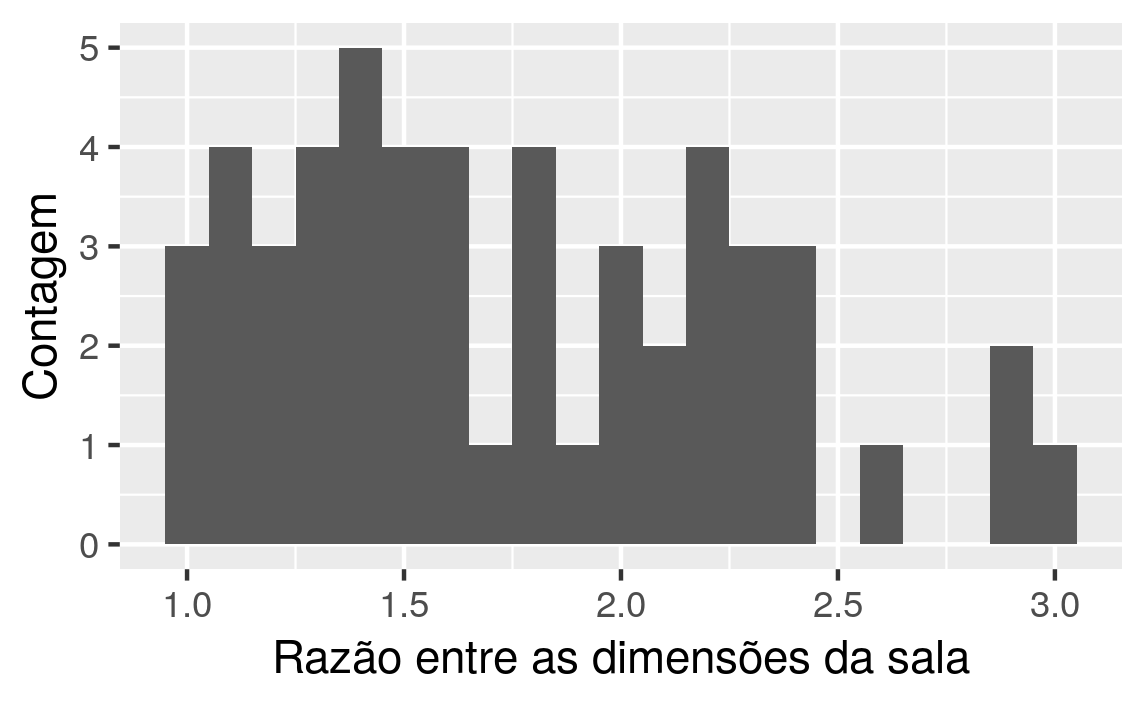
\includegraphics[width=\linewidth]{img/hist_ratio_sala.png}
	\end{minipage}%
%\end{figure}
%\begin{figure}
%	\ContinuedFloat
%	\caption[]{\textit{Continuação}} % {figure}
%	\centering	
	\begin{minipage}{.33\textwidth}
		\centering
		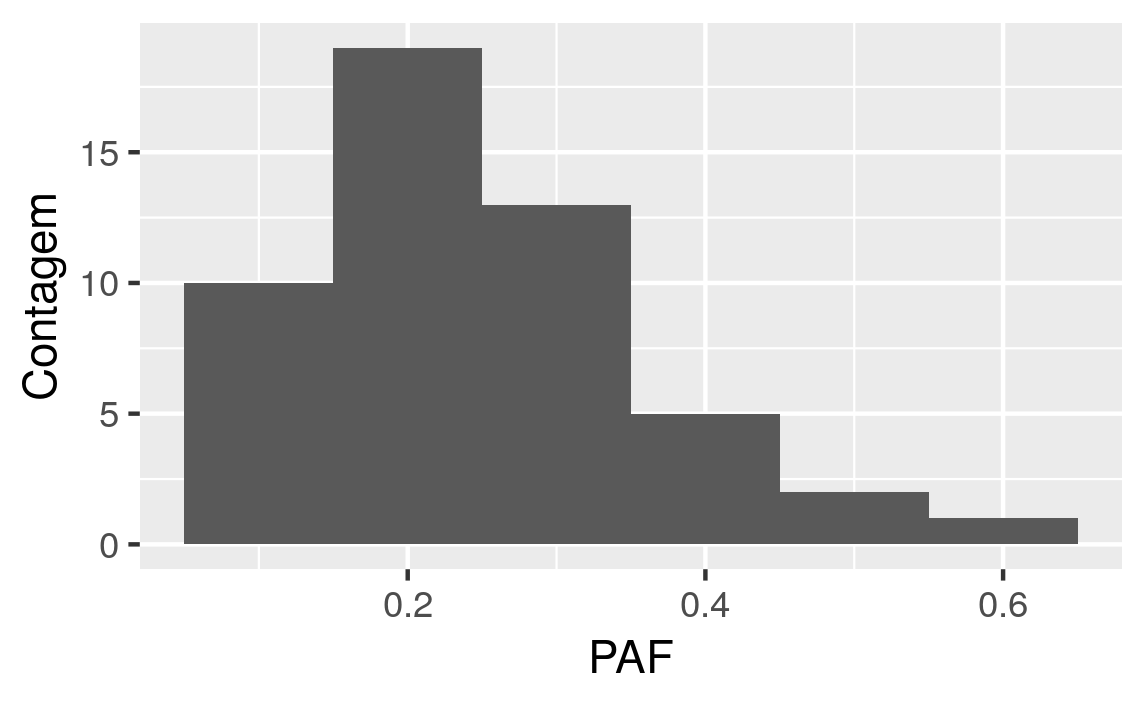
\includegraphics[width=\linewidth]{img/hist_PAF.png}
	\end{minipage}
	\centering
	\begin{minipage}{.33\textwidth}
		\centering
		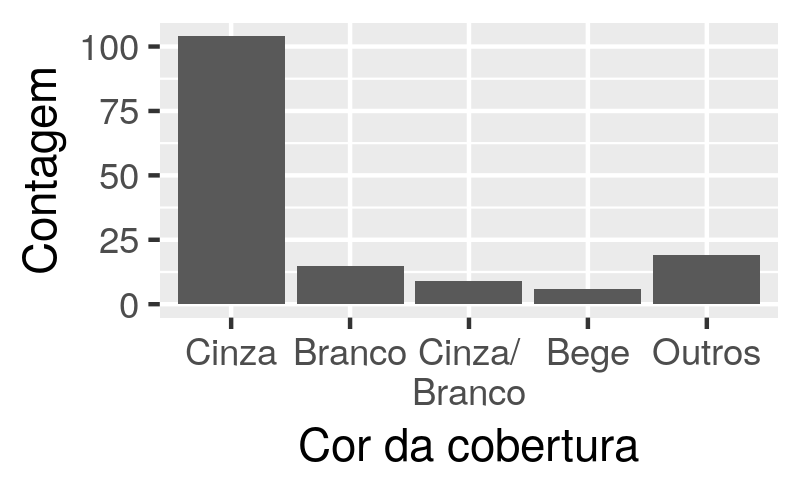
\includegraphics[width=\linewidth]{img/hist_cor_cobertura.png}
	\end{minipage}%
	\begin{minipage}{.33\textwidth}
		\centering
		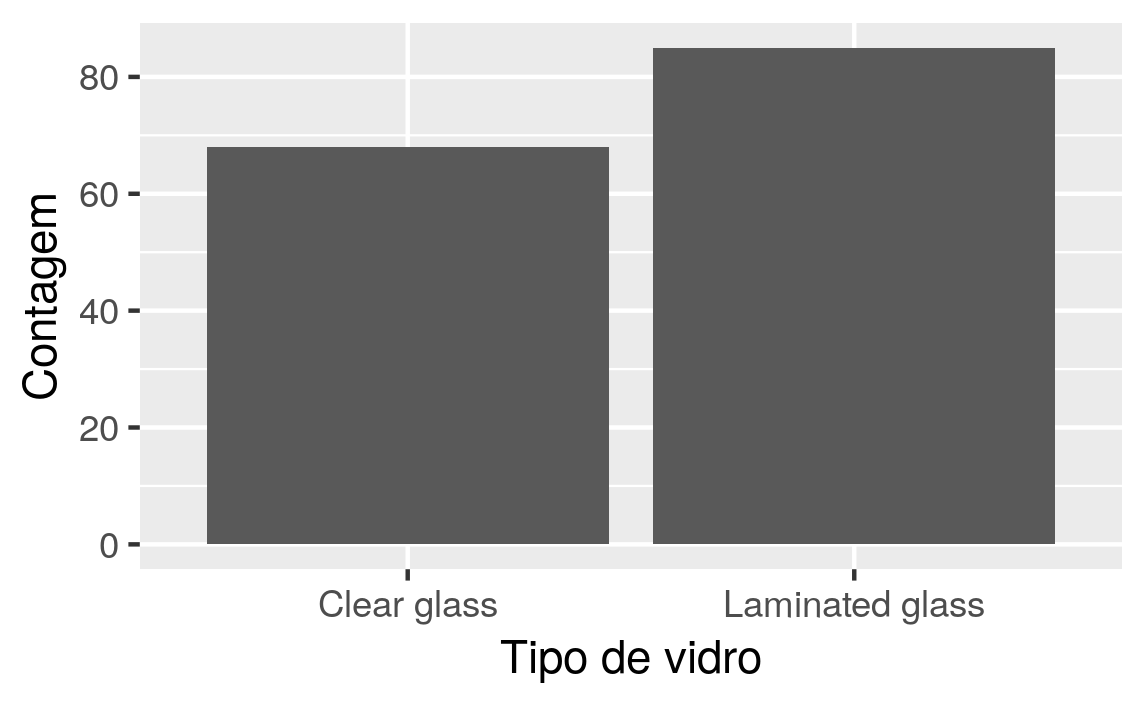
\includegraphics[width=\linewidth]{img/hist_tipo_vidro.png}
	\end{minipage}%
	\begin{minipage}{.33\textwidth}
		\centering
		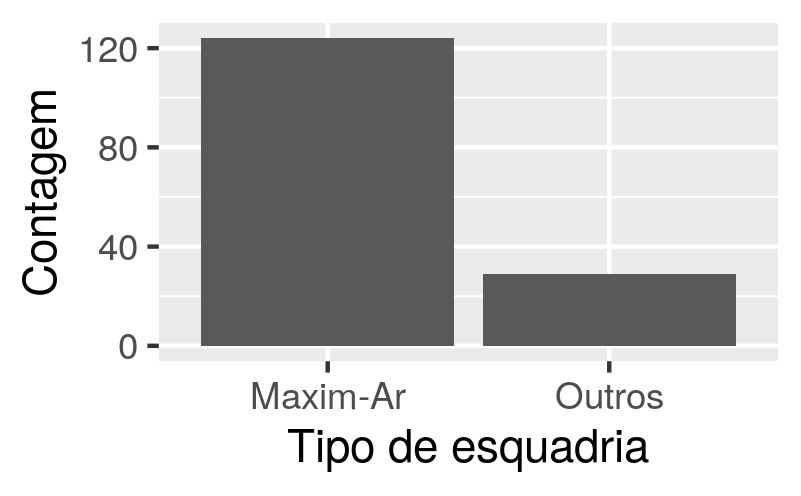
\includegraphics[width=\linewidth]{img/hist_esquadria.png}
	\end{minipage}
	\centering	
	\begin{minipage}{.33\textwidth}
		\centering
		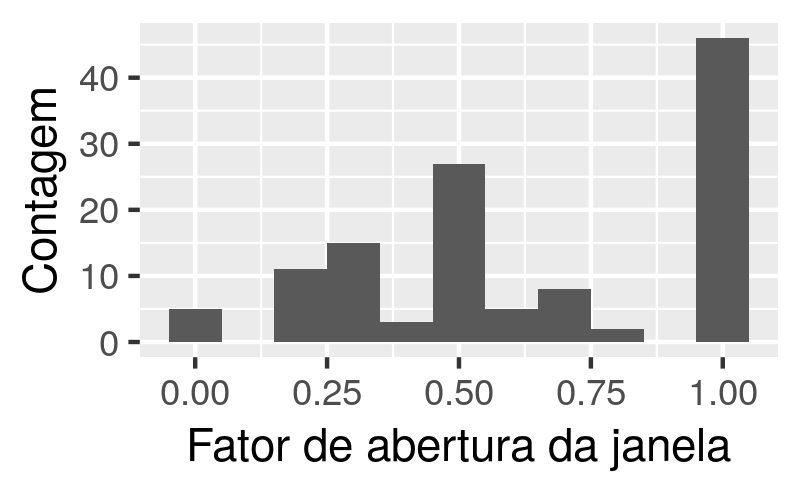
\includegraphics[width=\linewidth]{img/hist_openfac.png}
	\end{minipage}%
	\begin{minipage}{.33\textwidth}
		\centering
		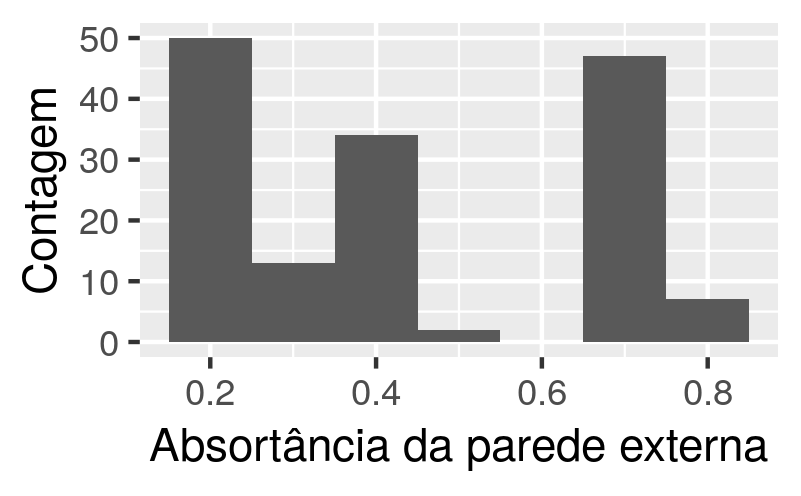
\includegraphics[width=\linewidth]{img/hist_absortancia.png}
	\end{minipage}%
	\begin{minipage}{.33\textwidth}
		\centering
		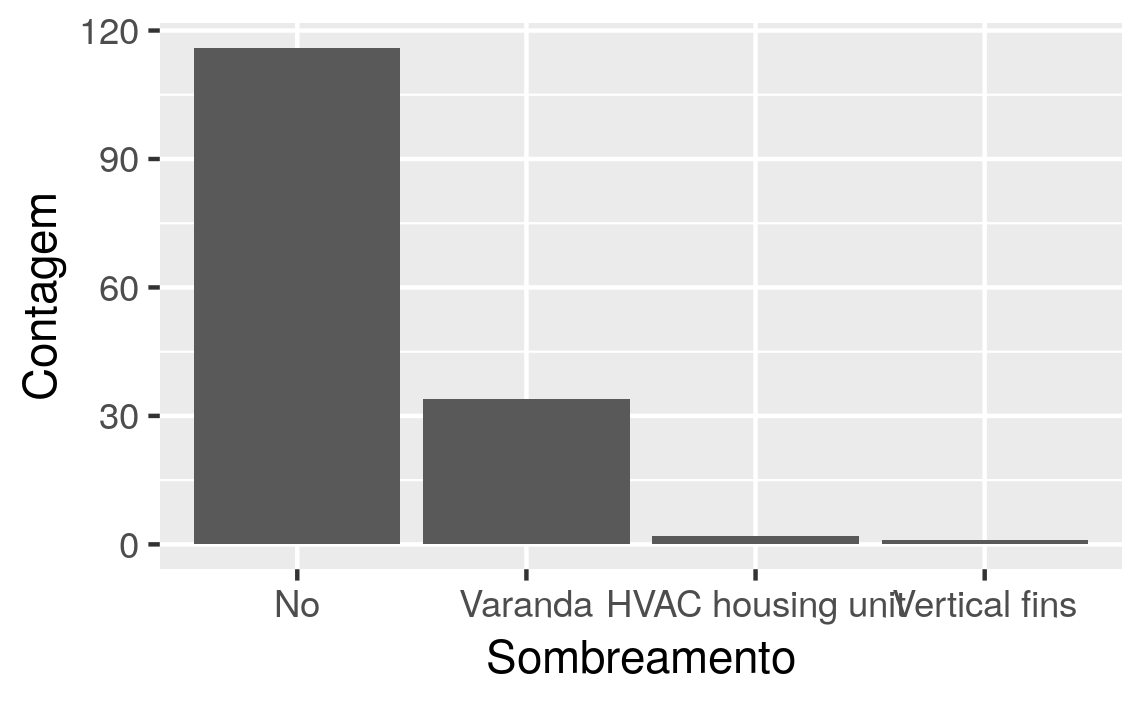
\includegraphics[width=\linewidth]{img/hist_sombreamento.png}
	\end{minipage}
%	\centering
	\begin{minipage}{.33\textwidth}
%		\centering
		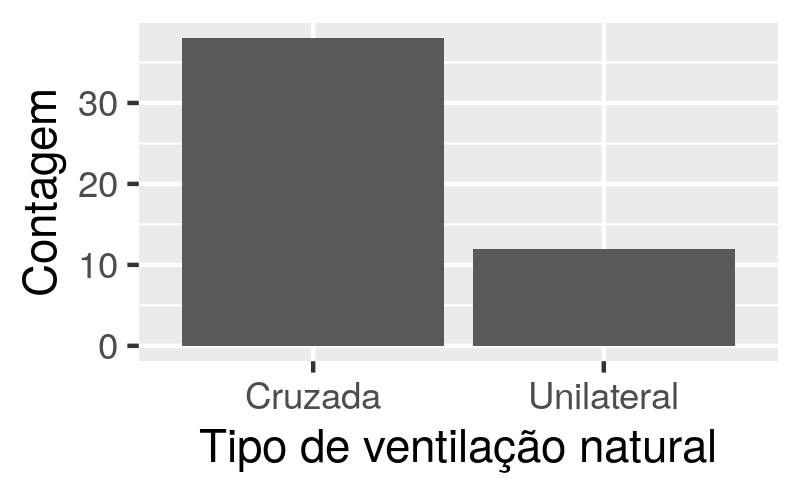
\includegraphics[width=\linewidth]{img/hist_tipo_vn.png}
	\end{minipage}
\end{figure}
\newpage

O ângulo do azimute é medido em relação ao eixo mais longo das edificações. Observou-se que há ângulos em diversas orientações, indicando que não existe uma orientação predominantemente escolhida para a construção dos edifícios.
O número de pavimentos dos edifícios analisados varia entre 2 e 20 pavimentos, com a maioria das ocorrências em 12 pavimentos.
Tanto os edifícios, quanto as salas existentes no banco de dados apresentam predominantemente formato retangular, a partir do qual considera-se que definir as simulações baseando-se em modelos de edificações retangulares, com salas retangulares, representa adequadamente as tipologias de edifícios encontradas na cidade de São Paulo.
A altura do pé direito não varia significativamente, mas tem a maioria das ocorrências em volta de 2,5 m.
A área das salas de escritório varia entre, aproximadamente, 25 m$^2$ e 160 m$^2$, com a maior ocorrência em valores próximos a 40 m$^2$.
As proporções entre as suas menores e maiores dimensões variam entre, aproximadamente, 0,3 e 1, mas a maior ocorrência está próxima ao valor 0,6.
As proporções entre as menores e maiores dimensões dos pavimentos varia consideravelmente, entre 0,1 e 1.

A absortância das paredes dos edifícios varia entre 0,2 e 0,8, de forma distribuída entre absortâncias baixas, médias e altas. A cor das coberturas é predominantemente cinza. Portanto, foi definido o valor fixo de 0,7 para absortância da cobertura.

Observou-se que esquadrias do tipo maxim-ar são predominantes. Os objetos do \textit{Airflow Network} do programa EnergyPlus não modelam especificamente este tipo de esquadria. Porém, optou-se por considerar as janelas como não pivotantes. Considerar uma janela como horizontalmente pivotante implicaria na consideração de que a abertura acontece simultaneamente na parte de cima e de baixo da janela. No caso da janela maxim-ar, por mais que a abertura aconteça em um eixo horizontal, apenas a parte inferior da janela se abre. 
Os fatores de abertura variam entre zero e um. No entanto, não é aplicável janelas com fatores de abertura igual a zero para edificações com \acrshort{vn}.
O \acrfull{paf} varia entre 0,1 e 0,6 aproximadamente.

O uso de elementos de sombreamento é pouco explorado nas edificações existentes. De qualquer maneira, considerou-se a modelagem de sombreamento horizontal sobre as aberturas da edificação, por considerar o potencial do sombreamento para bloquear a entrada de radiação nas zonas térmicas simuladas. Esse parâmetro foi variado a partir do ângulo de sombreamento formado entre a base da abertura e a proteção solar, localizada no topo da abertura.	
A maioria das salas observadas possuem ventilação cruzada, mas a ventilação unilateral é uma estratégia com ocorrência considerável.

As informações relacionadas ao tipo de vidro não permitem definir valores relacionados ao \acrfull{fs}. Observa-se apenas a ocorrência de vidros laminados e vidro comum incolor. Optou-se por variar o fator solar dos vidros nas simulações para avaliar o impacto deste parâmetro nos resultados de conforto térmico.

%	Os demais parâmetros observados tiveram suas distribuições variando continuamente de acordo com as distribuições obtidas. 
Como as simulações detalhadas foram modeladas como pavimentos da edificação, o parâmetro relacionado ao número de pavimento das edificações foi transformado no parâmetro "altura do pavimento", ou seja, um pavimento localizado em um andar $n$, com um pé-direito de dimensão $h$, foi considerado com uma altura do pavimento igual a $n{\cdot}h$.

A definição dos parâmetros de entrada para o desenvolvimento do metamodelo foi baseada no banco de dados analisados. A Tabela \ref{table:param_def} apresenta os limites mínimos e máximos atribuídos aos diferentes parâmetros contínuos variados nas simulações, assim como os parâmetros variados pela lógica "sim/não". A velocidade do ar foi variada com valores discretos, de acordo com os valores definidos pela \citeonline{ASHRAEStandard552017}, apresentados na Tabela \ref{table:var} do Capítulo \ref{chapter:metodologia}.

\begin{table}[H]
	\centering
	\caption{Limites mínimos e máximos dos parâmetros}
	\label{table:param_def}	
%	\resizebox{\textwidth}{!}{
	\begin{tabular}{|l |r |}
		\hline
		\textbf{Parâmetro} & \textbf{Valores} \\
		\hline
		Área da sala ($m^2$) & 20 - 100 \\
		\hline
		Razão entre maior e menor da sala ($-$) & 0,4 - 2,5 \\
		\hline
%		Razão entre maior e menor  & {} \vspace{-7pt}\\
%		{} & 0,4 - 2,5 \vspace{-7pt}\\ 
%		da sala ($-$) & {} \\
%		\hline
		Pé-direito ($m$) & 2,3 - 3,2 \\
		\hline
		Azimute ($^{\circ}$) & 0 - 360 \\
		\hline
		Altura do pavimento ($m$) & 0 - 50 \\
		\hline 
		Absortância da parede ($-$) & 0,2 - 0,8 \\
		\hline 
		Transmitância da parede ($W/m^2K$) & 0,5 - 4,4 \\
		\hline 
		Capacidade térmica da parede ($kJ/m^2K$) & 0,22 - 450,00 \\
		\hline 
		\Acrlong{paf} ($-$) & 0,1 - 0,6 \\
		\hline 
		Fator solar do vidro ($-$) & 0,20 - 0,87 \\
		\hline 
		Sombreamento ($^{\circ}$) & 0 - 80 \\
		\hline 
		Densidade de ocupação ($pessoa/m^2$) & 0,05 - 0,20 \\
		\hline 
		Fator de abertura da janela ($-$) & 0,2 - 1,0 \\
		\hline 
		Razão entre maior e menor dimensão do edifício ($-$) & 0,2 - 1,0 \\
		\hline 
		Cobertura exposta & Sim / Não\\
		\hline 
		Piso exposto & Sim / Não\\
		\hline 
		Ventilação & Cruzada / Unilateral\\
		\hline 
		Velocidade do ar ($m/s$) & 0,0 - 1,2 \\
		\hline 
	\end{tabular}
%}
	%			\begin{flushleft}
	%				Fonte: \citeauthoronline{INIC} \cite{INIC}, adaptado pelo autor.
	%			\end{flushleft}				
\end{table}

\section{Simulações simplificadas}

\subsection{Cálculo do coeficiente de pressão pelo método analítico}

Ao comparar os valores dos \acrfull{cp} das medições em túnel de vento da \acrfull{tpu} e os valores dos \acrshort{cp} obtidos pelo \acrlong{ma}, obteve-se gráficos de pontos. 
A Figura \ref{fig:cp_diff_scatter}a apresenta a comparação para as 25 proporções geométricas disponibilizadas pela \acrshort{tpu}, para cada fachada, e para cada ponto na fachada.
Como os valores calculados pelo \acrlong{ma} são únicos para cada fachada, e a \acrshort{tpu} oferece valores diferentes para diversos pontos ao longo das fachadas, os pontos no gráfico da Figura \ref{fig:cp_diff_scatter} distribuem-se horizontalmente. 
%		A Figura \ref{fig:cp_diff_scatter_facade} apresenta a comparação considerando-se os valores médios do \acrshort{cp} para cada fachada. 
É possível observar que a faixa de valores dos \acrshort{cp} disponibilizados pela \acrshort{tpu} é maior do que  faixa de valores calculados pelo \acrlong{ma}. Enquanto o menor valor de \acrshort{cp} disponibilizado pela \acrshort{tpu} é \mbox{-1,40}, e o maior valor é 1,08, pelo \acrlong{ma} o valor mínimo é igual a -0,96 e o máximo é igual a 0,60.

Dentre as geometrias analisadas, a proporção com a maior \gls{rmsecp} entre os valores dos \acrshort{cp} foi igual a 0,42, para a geometria da edificação \textit{highrise} com proporções de largura, profundidade e altura igual a 2:1:2 (Figura \ref{fig:cp_diff_scatter}b).

\vspace{40pt}
\newpage

\begin{figure}[h]
%	\centering
	\caption{Comparação entre os valores de $C_p$ obtidos pelo método analítico e pela base de dados da TPU}
	\begin{minipage}{.5\textwidth}
%		\centering
		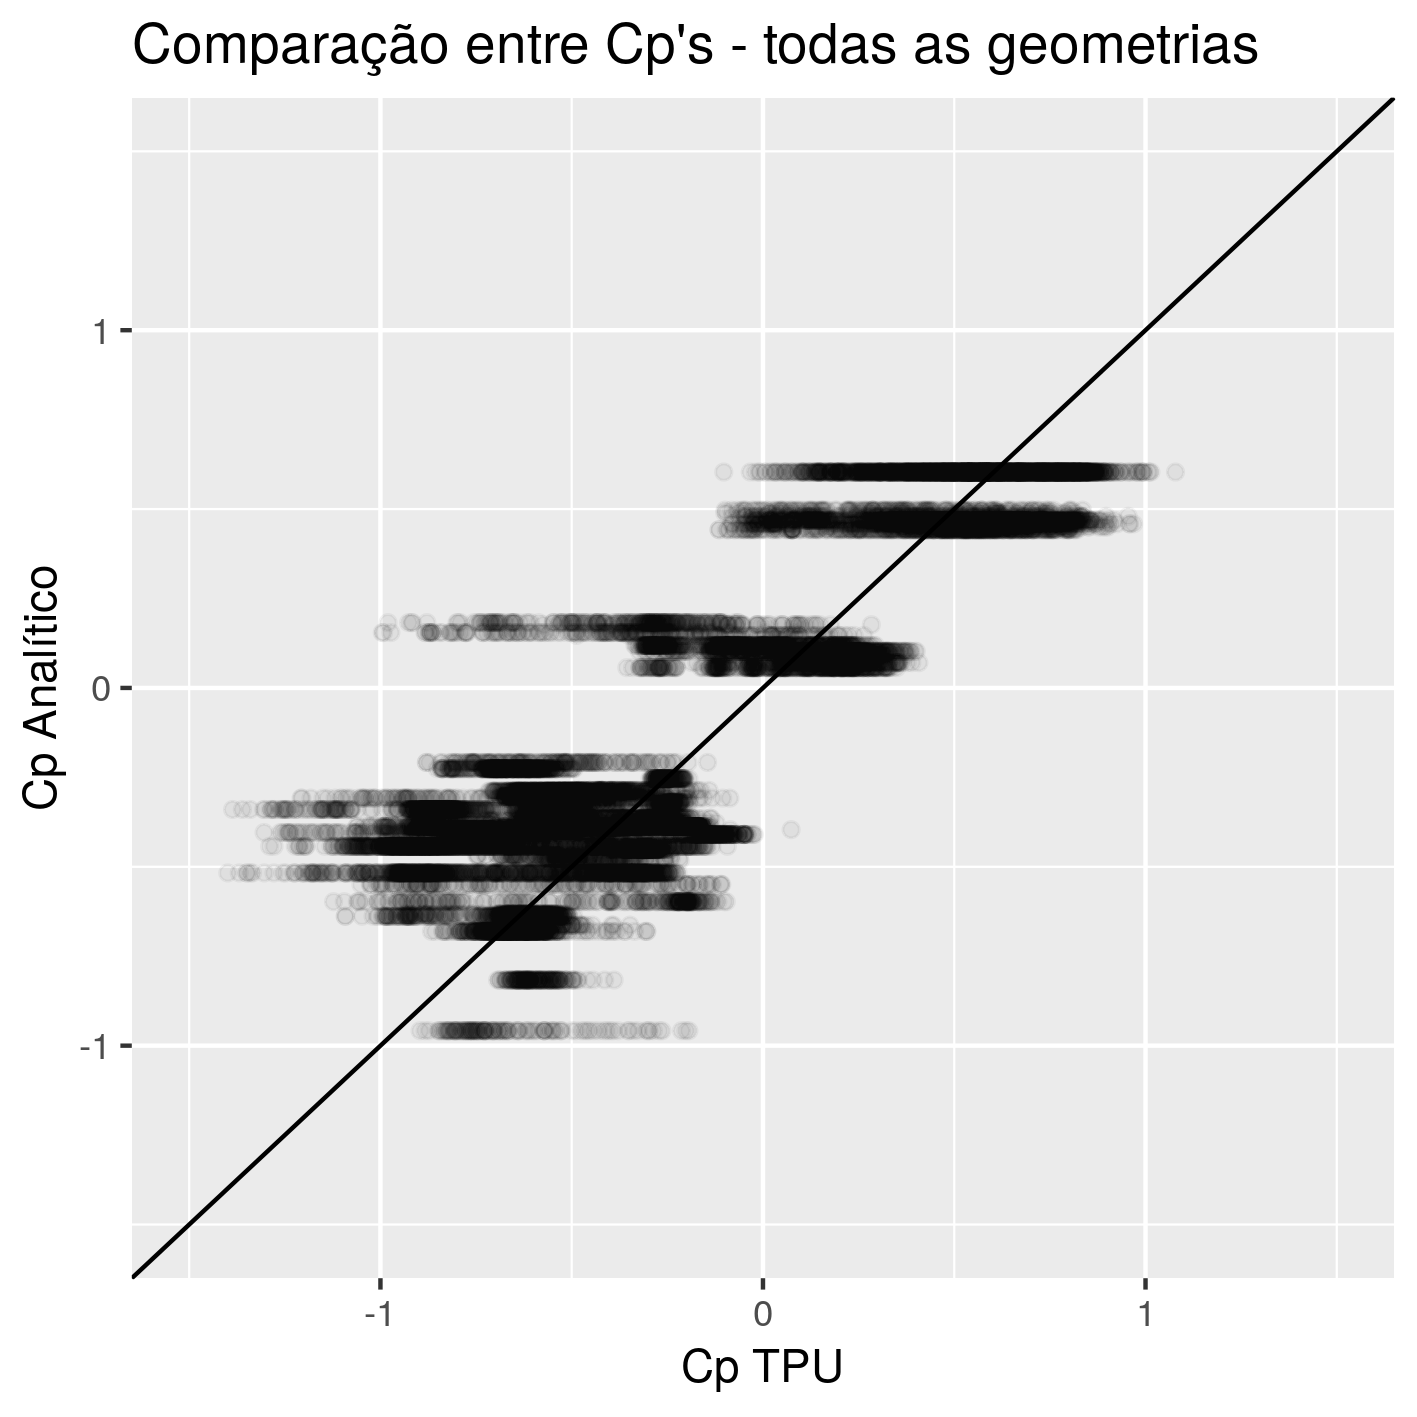
\includegraphics[width=\linewidth]{img/cp_diff_scatter_all.png}
%		\caption{Comparação entre os valores de \acrshort{cp} das 25 geometrias}
	\begin{center}
		\small{(a) Geometrias de todas as proporções disponíveis}
	\end{center}
	\end{minipage}%
	\begin{minipage}{.5\textwidth}
%		\centering
		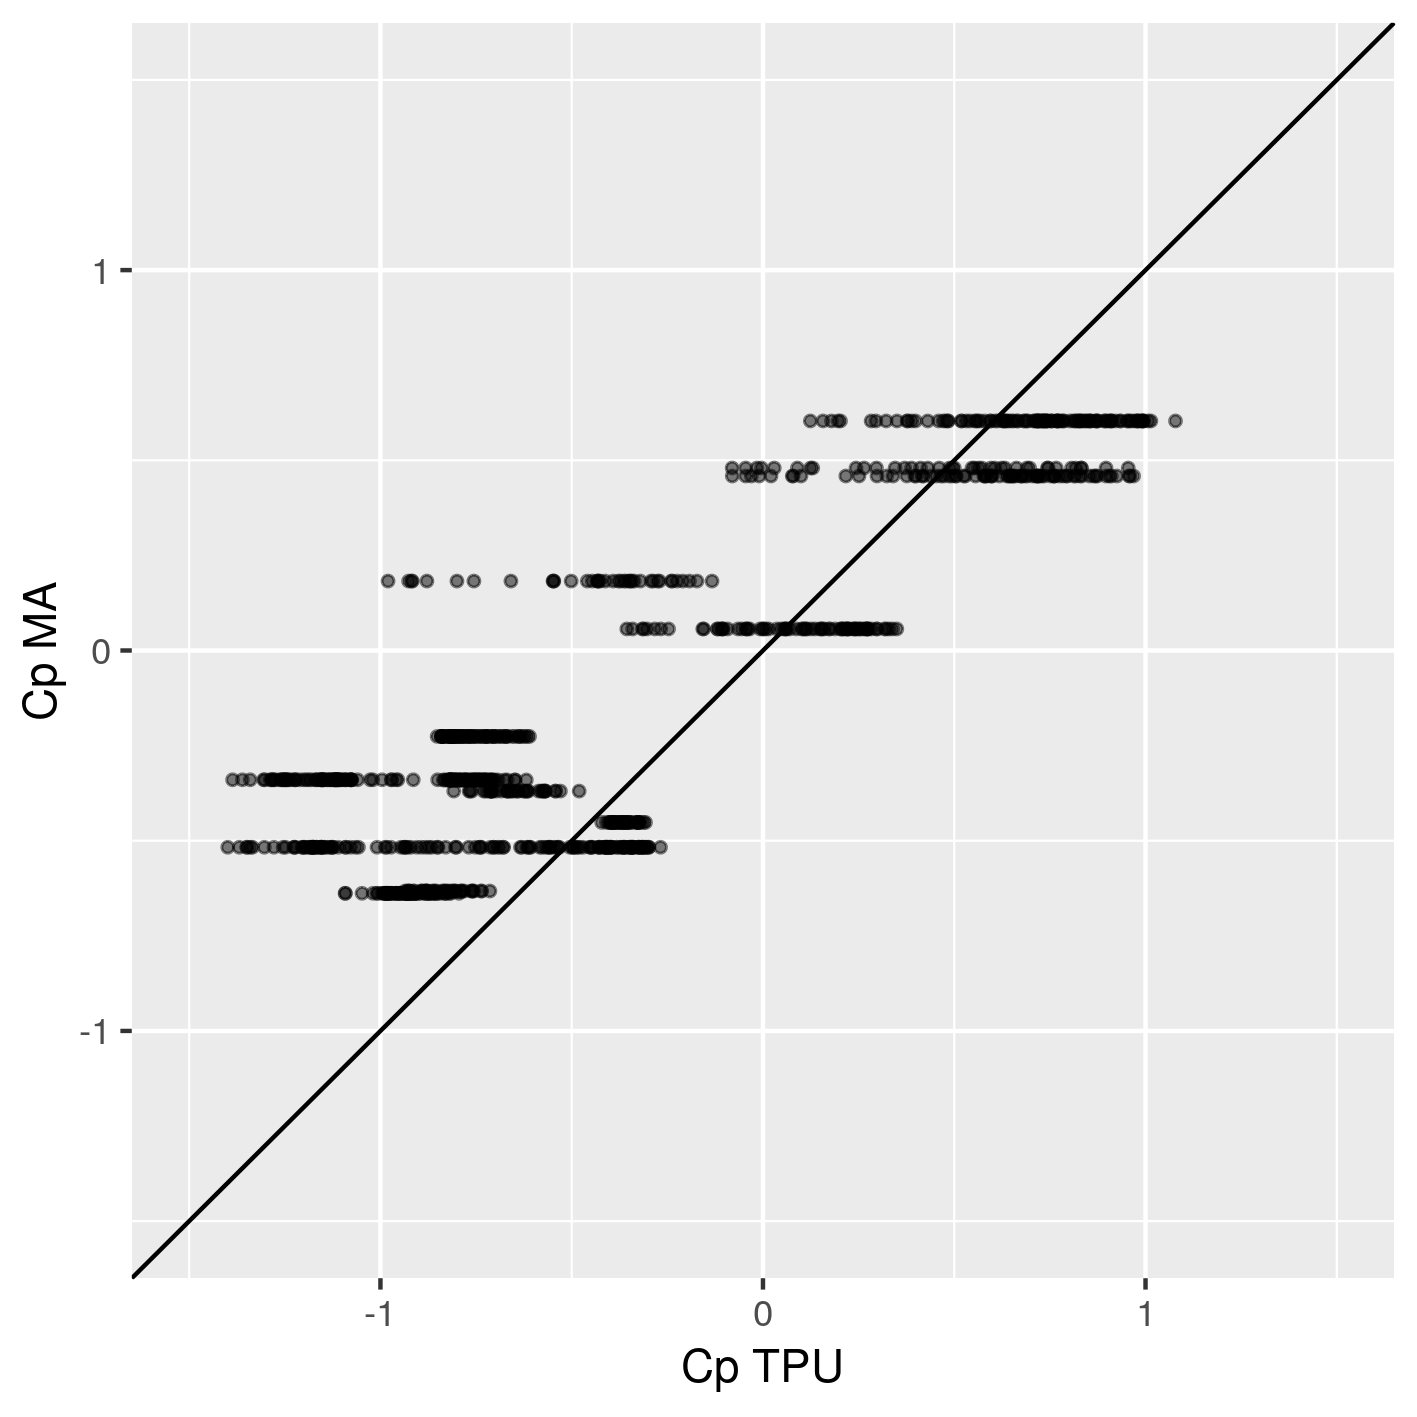
\includegraphics[width=\linewidth]{img/cp_diff_scatter.png}
%		\caption{Comparação entre os valores de \acrshort{cp} das 25 geometrias}
	\begin{center}
		\small{(b) Geometria de proporções 2:1:2}\\
		\phantom{}		
	\end{center}
	\end{minipage}
	\label{fig:cp_diff_scatter}
\end{figure}

%A partir do resultado da comparação dos \acrshort{cp} nas diferentes geometrias,  
Partindo-se de uma tipologia com proporções de largura, profundidade e altura igual a 2:1:2, as diferenças nos resultados de simulações termoenergéticas com \acrshort{cp} obtidos pelos diferentes métodos foram avaliadas. 
A Figura \ref{fig:cpaverage_ACH_scatter} apresenta a comparação entre as médias anuais de \acrfull{ach}. %, apresentada na ,

\begin{figure}[H]
	\centering
	\caption{Comparação das médias anuais de ACH utilizando-se o método analítico e a base de dados da TPU}
	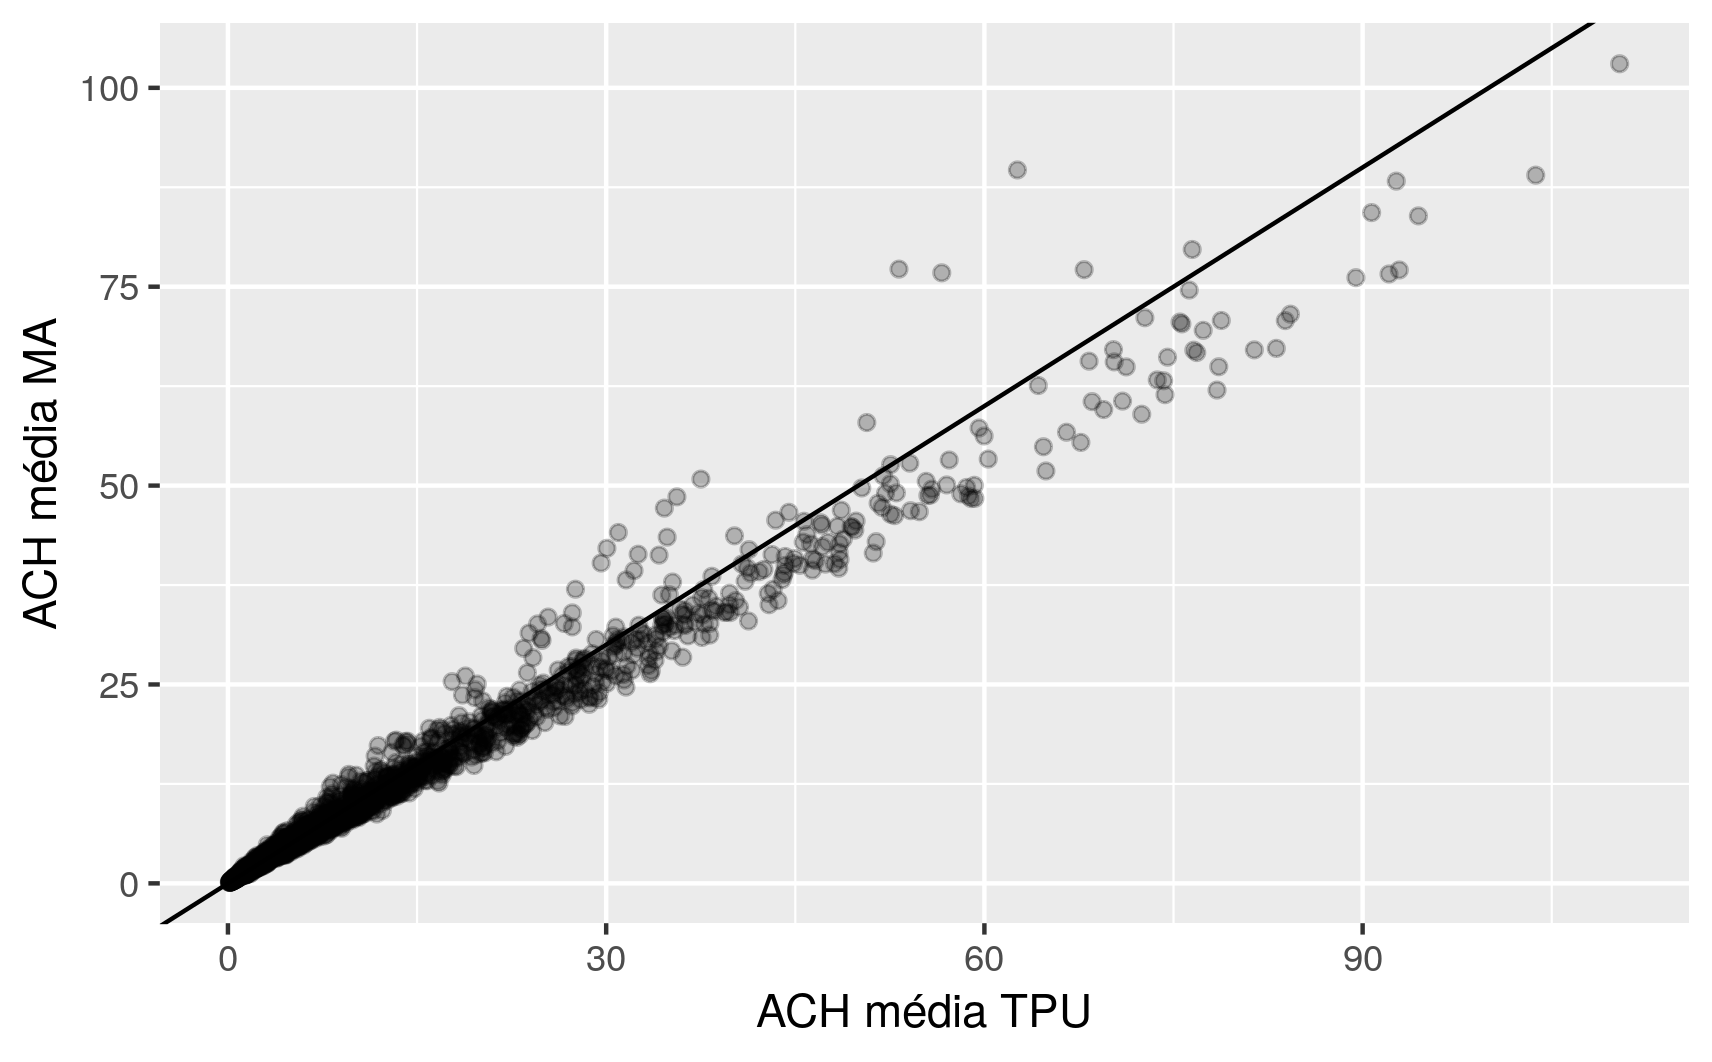
\includegraphics[width=.5\linewidth]{img/cpaverage_ACH_scatter.png}
	\label{fig:cpaverage_ACH_scatter}
	%			\begin{flushleft}
	%				Fonte: o autor.
	%			\end{flushleft}
\end{figure}

A comparação entre as médias anuais de \acrshort{ach} mostra que o \acrlong{ma} faz com que as trocas de ar sejam predominantemente subestimadas nas simulações, possivelmente devido aos menores valores dos \acrshort{cp} obtidos pelo método.
A diferença média foi igual a 0,56 \acrshort{ach}, com o \acrfull{ae95} é igual a 5,23 \acrshort{ach}.

Apesar dessas diferenças nas trocas de ar, a comparação entre as temperaturas operativas médias, apresentada na Figura \ref{fig:cpaverage_tempEHF_scatter}a, mostra que a diferença média da temperatura operativa é 0,04 $^{\circ}$C, sendo que o \acrshort{ae95} é igual a 0,31 $^{\circ}$C.
Essas diferenças são confirmadas como pouco significativas ao se analisar a Figura \ref{fig:cpaverage_tempEHF_scatter}b, com a comparação da \acrfull{ehf}. A média de diferença do \acrshort{ehf} nos casos analisados foi igual a 0,0037, com o \acrshort{ae95} igual a 0,0277.
Portanto, considerou-se que a utilização do \acrlong{ma} para calcular os valores dos \acrshort{cp} é uma alternativa adequada para a simplificação das simulações termoenergéticas.

\begin{figure}[h]
	\centering
	\caption{Comparação de temperaturas operativas e conforto térmico utilizando-se o método analítico e a base de dados da TPU}
	\begin{minipage}{.5\textwidth}
		\centering
		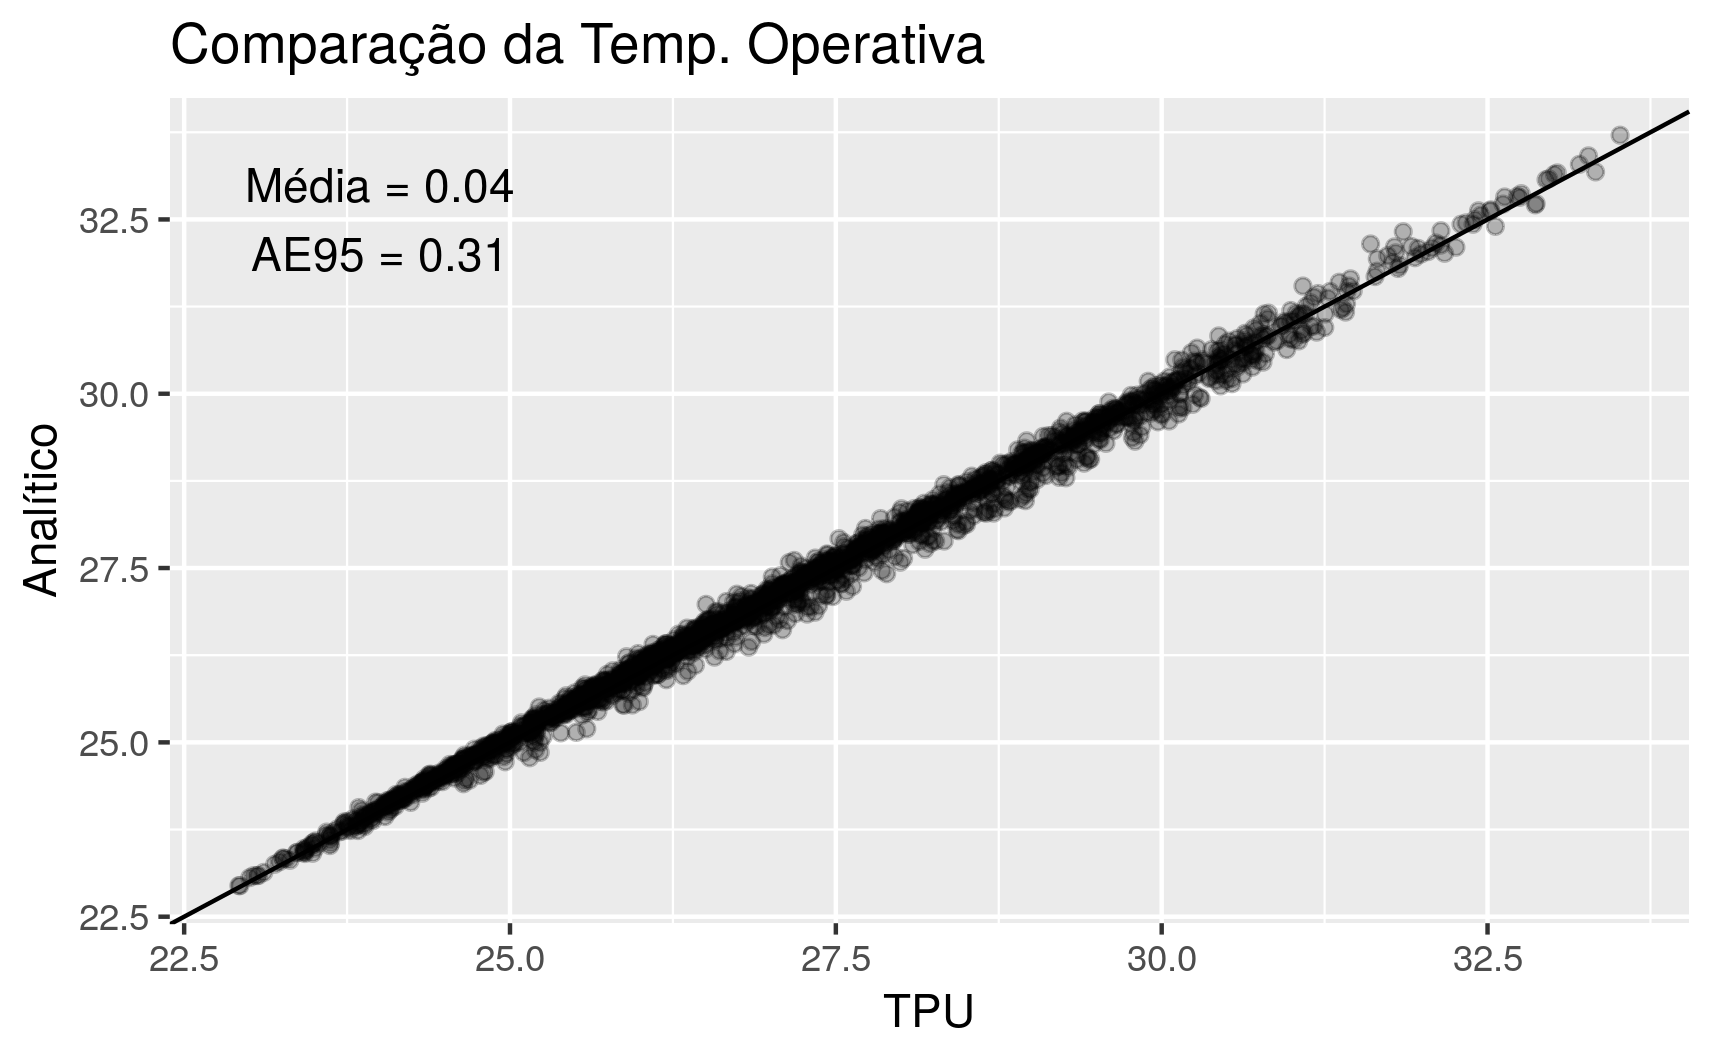
\includegraphics[width=\linewidth]{img/cpaverage_temp_scatter.png}
		%		\caption{Comparação entre os valores de \acrshort{cp} das 25 geometrias}
		\begin{center}
			\small{(a) média anual da temperatura operativa}
		\end{center}
	\end{minipage}%
	\begin{minipage}{.5\textwidth}
		\centering
		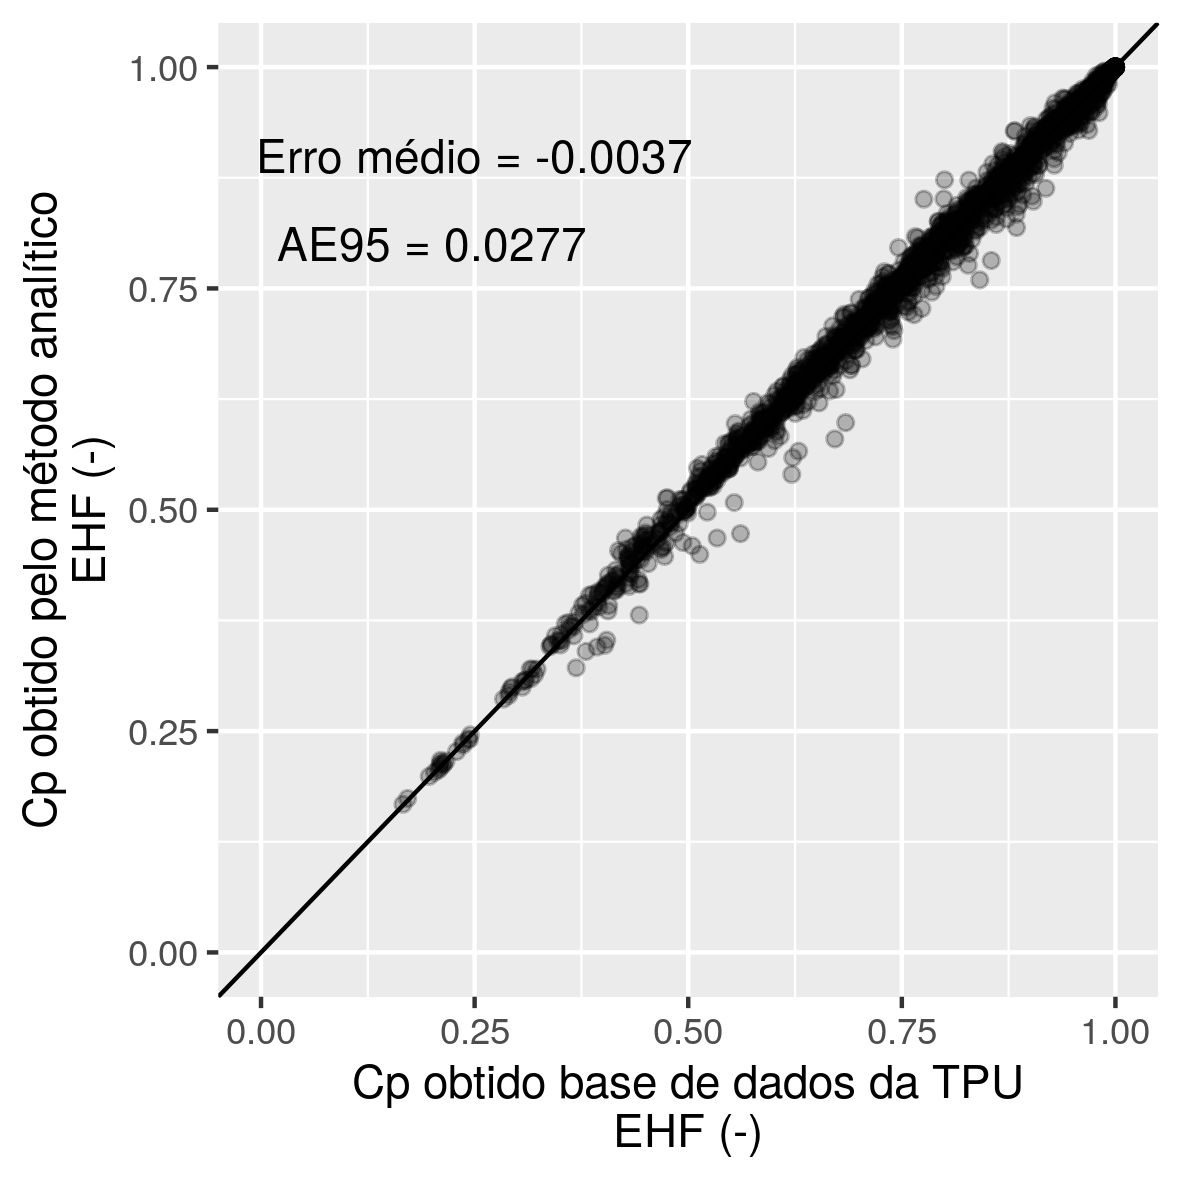
\includegraphics[width=\linewidth]{img/cpaverage_EHF_scatter.png}
		%		\caption{Comparação entre os valores de \acrshort{cp} das 25 geometrias}
		\begin{center}
			\small{(b) \acrlong{ehf}}
		\end{center}
	\end{minipage}
	\label{fig:cpaverage_tempEHF_scatter}
\end{figure}

%\begin{figure}[H]
%	\centering
%	\caption{Comparação entre as médias das temperaturas operativas}
%	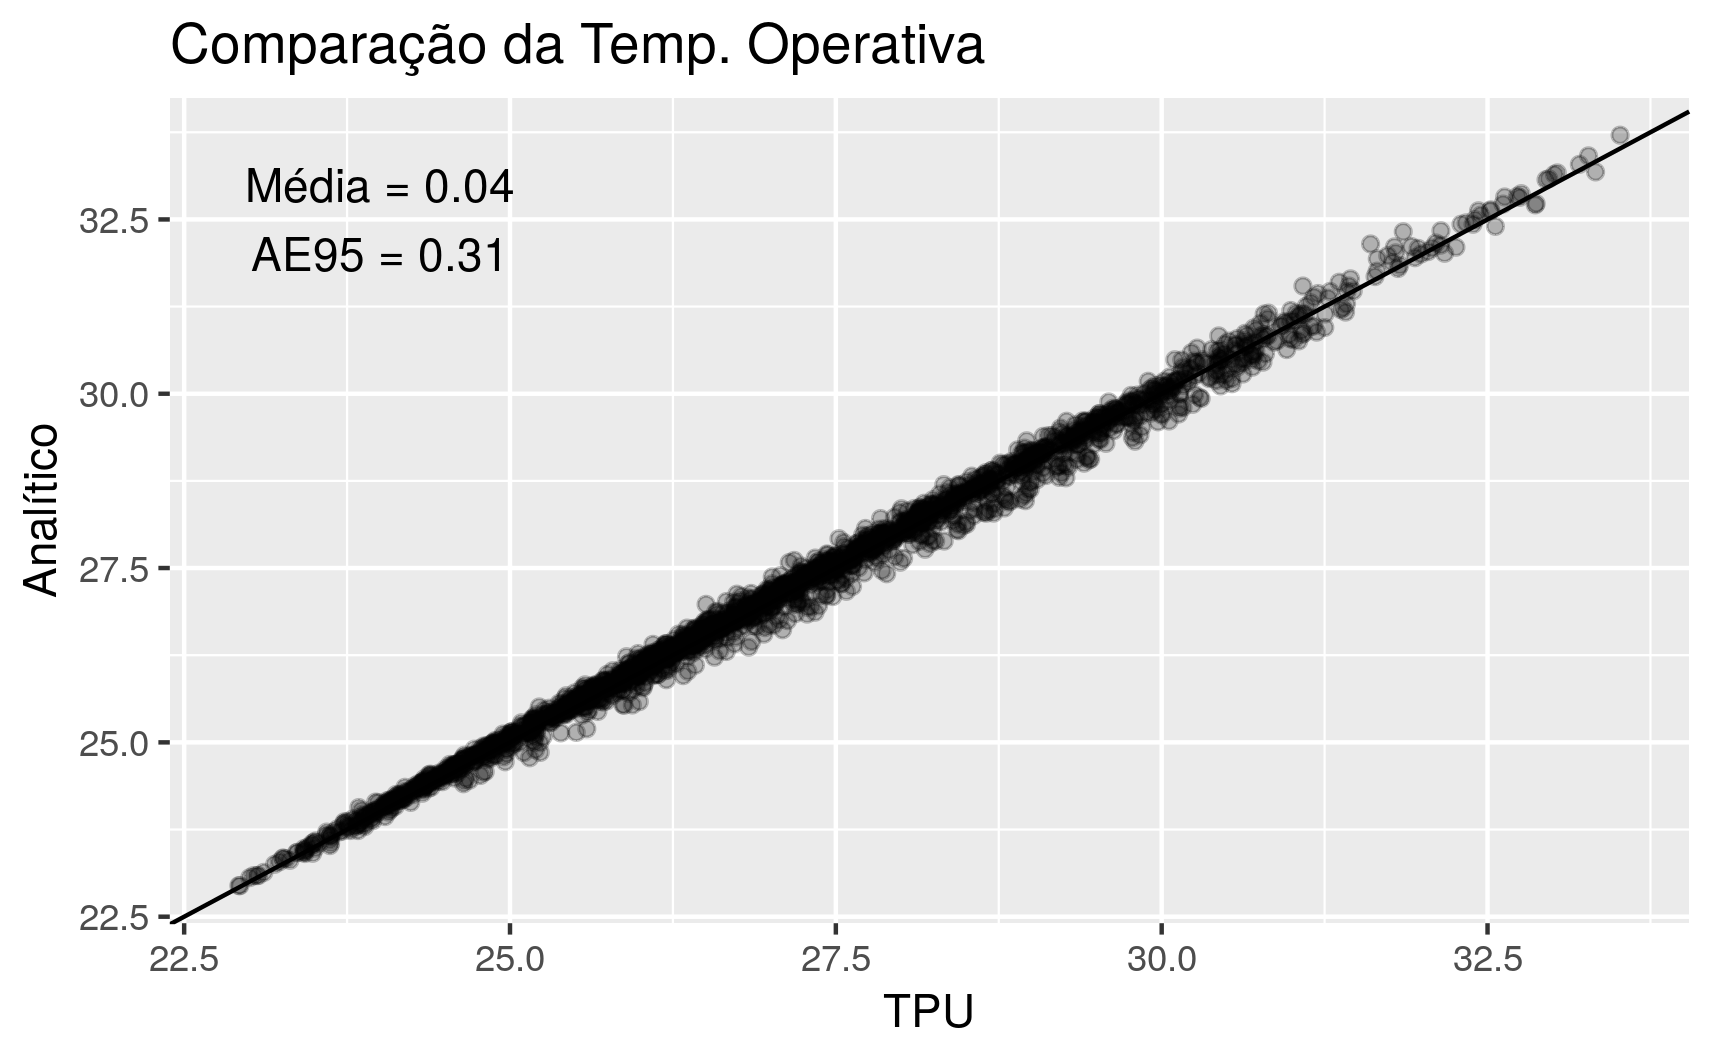
\includegraphics[width=\figsize\linewidth]{img/cpaverage_temp_scatter.png}
%	\label{fig:cpaverage_temp_scatter}
%	%			\begin{flushleft}
%	%				Fonte: o autor.
%	%			\end{flushleft}
%\end{figure}
%
%\begin{figure}[H]
%	\centering
%	\caption{Comparação entre os resultados de EHF}
%	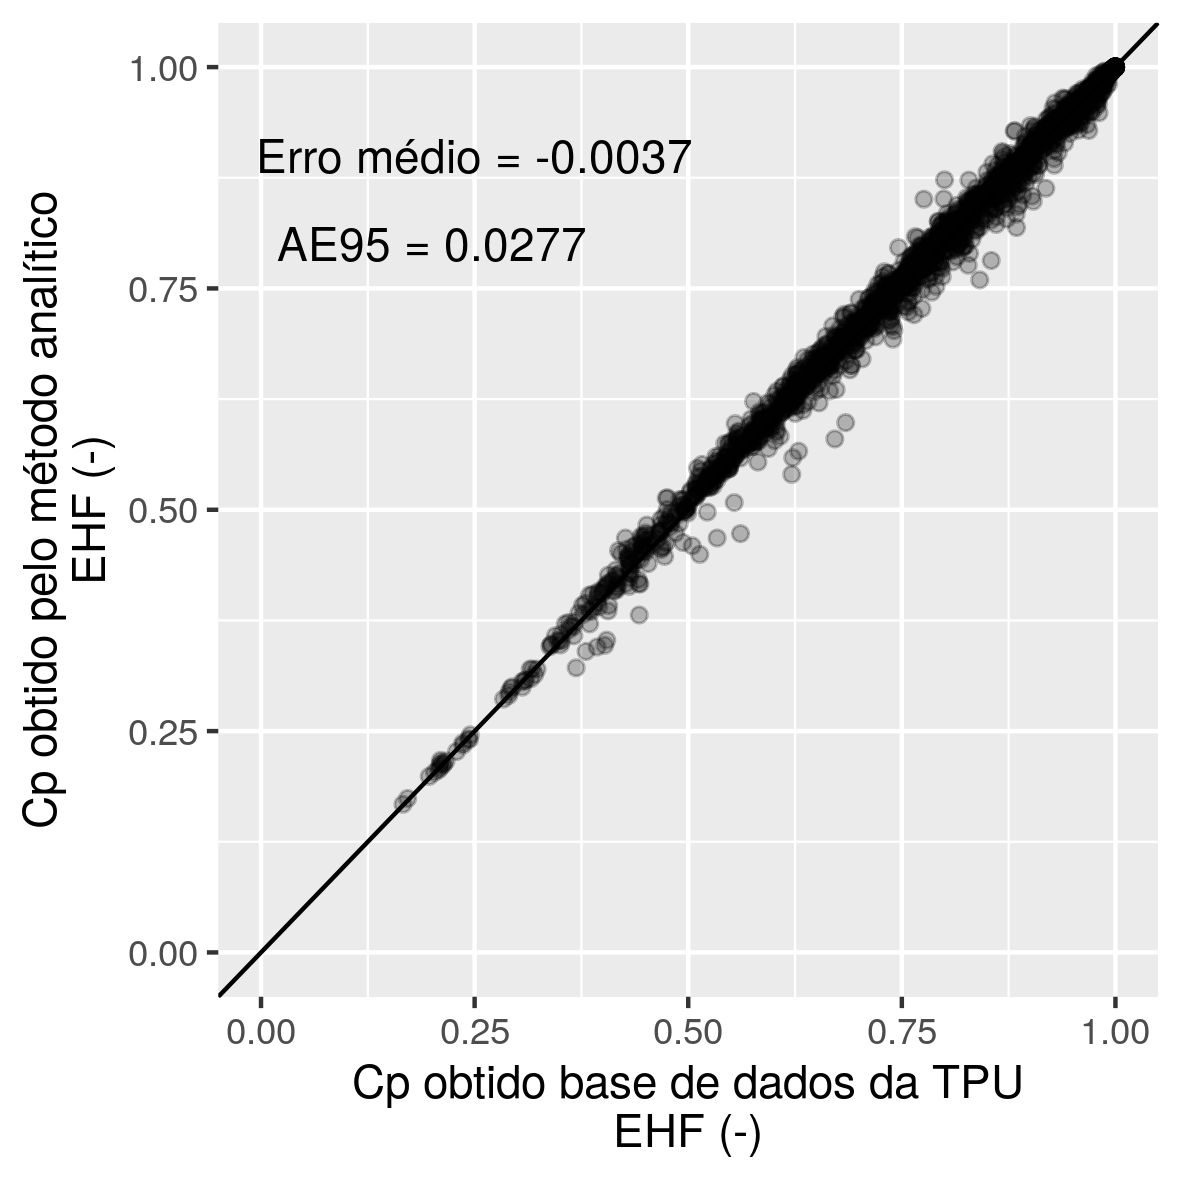
\includegraphics[width=\figsize\linewidth]{img/cpaverage_EHF_scatter.png}
%	\label{fig:cpaverage_EHF_scatter}
%	%			\begin{flushleft}
%	%				Fonte: o autor.
%	%			\end{flushleft}
%\end{figure}

\subsection{Representação da envoltória com duas camadas}

Os resultados das simulações com as paredes equivalentes subestimaram o \acrshort{ehf} em 0,0107 na média, quando comparados aos resultados das simulações com as paredes de referência. 
Os resultados das simulações para a parede de gesso com isolamento resultaram em um erro médio igual a 0,0099, e um \acrshort{ae95} igual a 0,0304 para o \acrshort{ehf} (Figura \ref{fig:par3_scatter}). O erro absoluto médio foi igual a 0,0100.

A representação da parede de alvenaria resultou em comportamentos semelhantes aos da parede de gesso com isoladamente.
Por mais que as diferenças sejam pouco expressivas, observou-se que utilizar o modelo de parede equivalente apresenta-se mais adequado considerando-se apenas metade do valor da \acrfull{ct} da parede. Enquanto que, para a parede equivalente com o valor total da capacidade térmica o erro médio foi igual a 0,0159, o \acrshort{ae95} foi igual a 0,0650, e o erro absoluto médio foi igual a 0,0209 (Figura \ref{fig:par2_scatter}a), para a parede equivalente com a metade do valor da capacidade térmica, o erro médio foi igual a 0,0115, o \acrshort{ae95} foi igual a 0,0604, e o erro absoluto médio foi igual a 0,0189 (Figura \ref{fig:par2_scatter}b).

\begin{figure}[h]
	\centering
	\caption{Comparação entre os resultados de EHF para a parede de gesso com isolamento}
	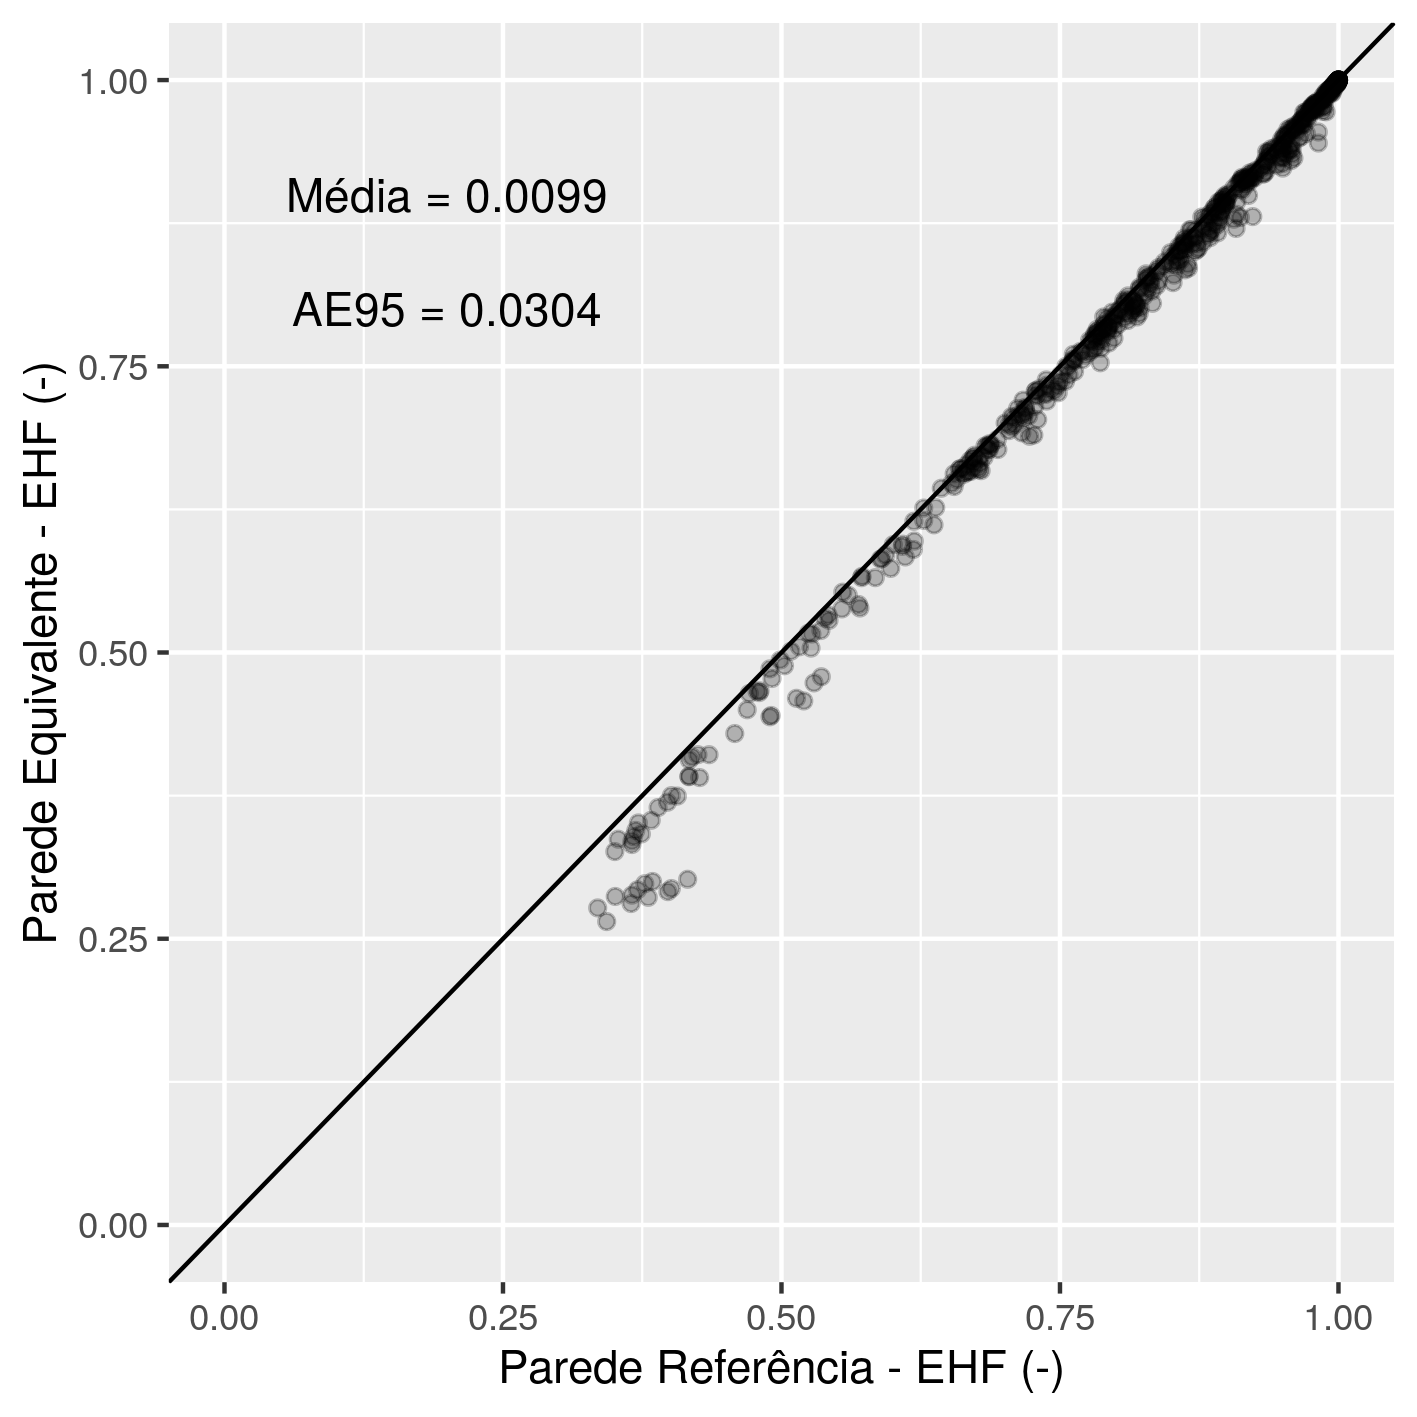
\includegraphics[width=.5\linewidth]{img/paredeeq_EHF_par3_scatter.png}
	\label{fig:par3_scatter}
	%			\begin{flushleft}
	%				Fonte: o autor.
	%			\end{flushleft}
\end{figure}

\begin{figure}[h]
	%	\centering
	\caption{Comparação entre os resultados de EHF para a parede de alvenaria}
	\begin{minipage}{.5\textwidth}
		%		\centering
		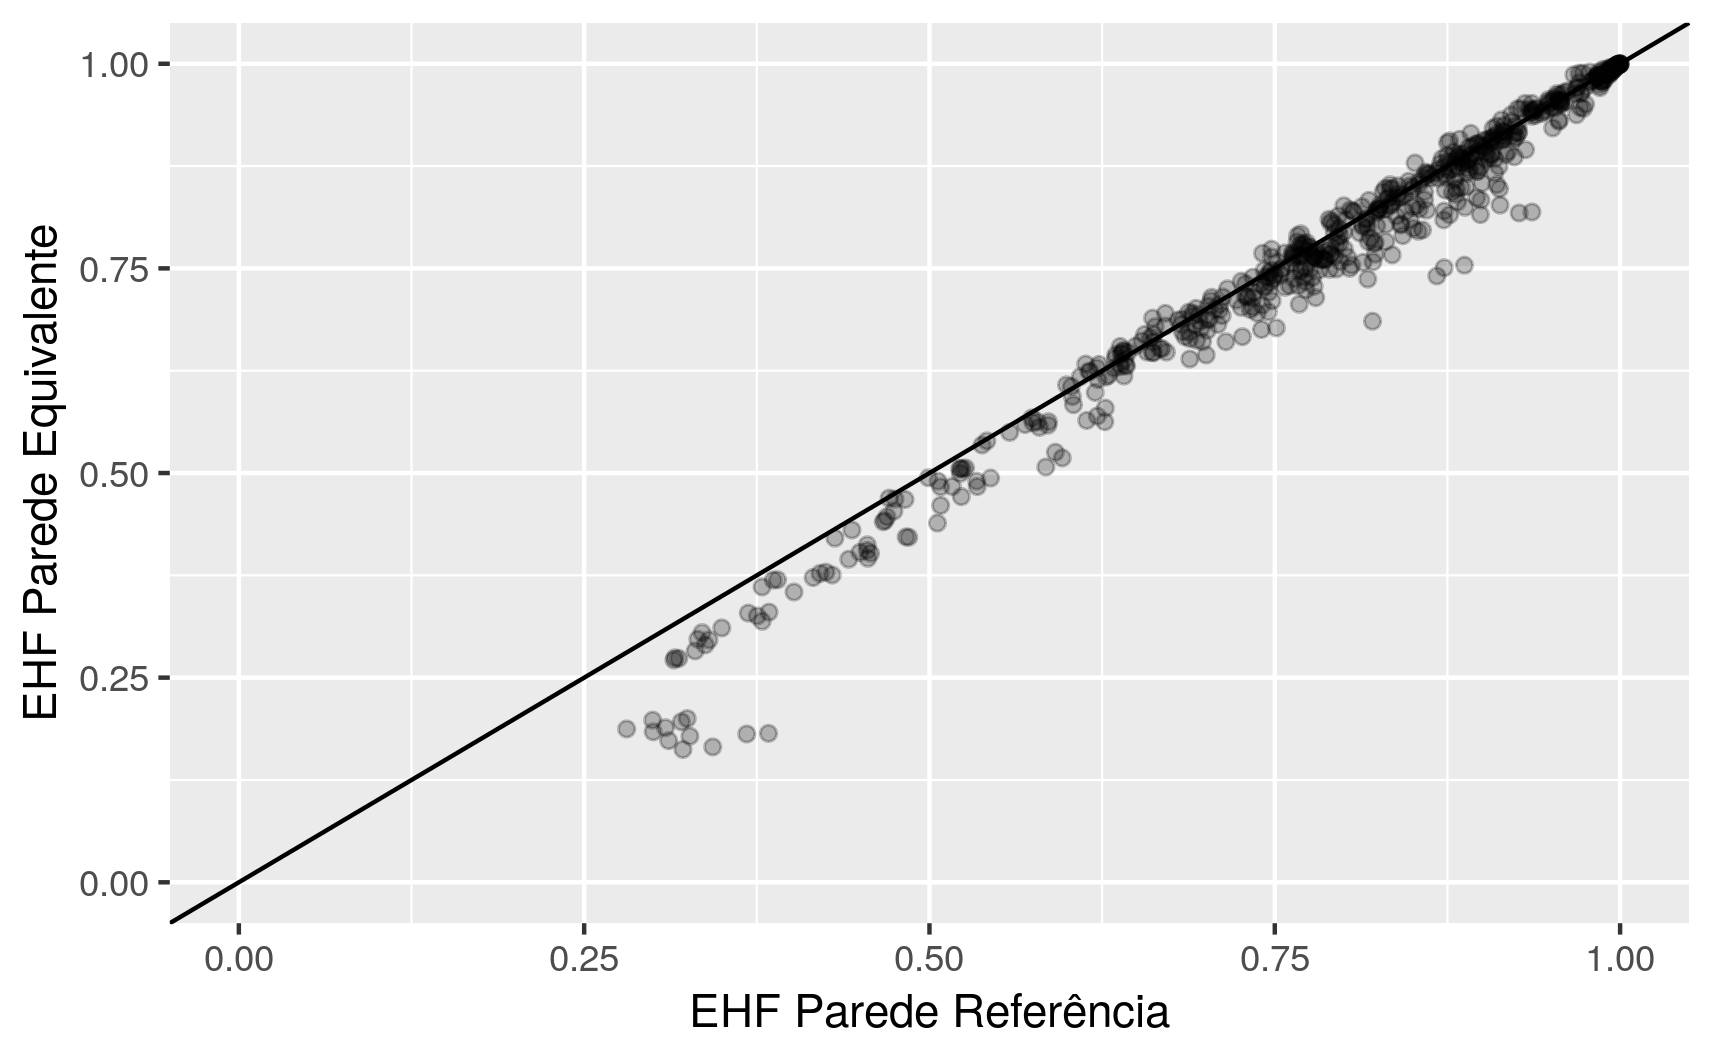
\includegraphics[width=\linewidth]{img/paredeeq_EHF_par2a_scatter.png}
		%		\caption{Comparação entre os valores de \acrshort{cp} das 25 geometrias}
		\begin{center}
			\small{(a) valor total da capacidade térmica}
		\end{center}
	\end{minipage}%
	\begin{minipage}{.5\textwidth}
		%		\centering
		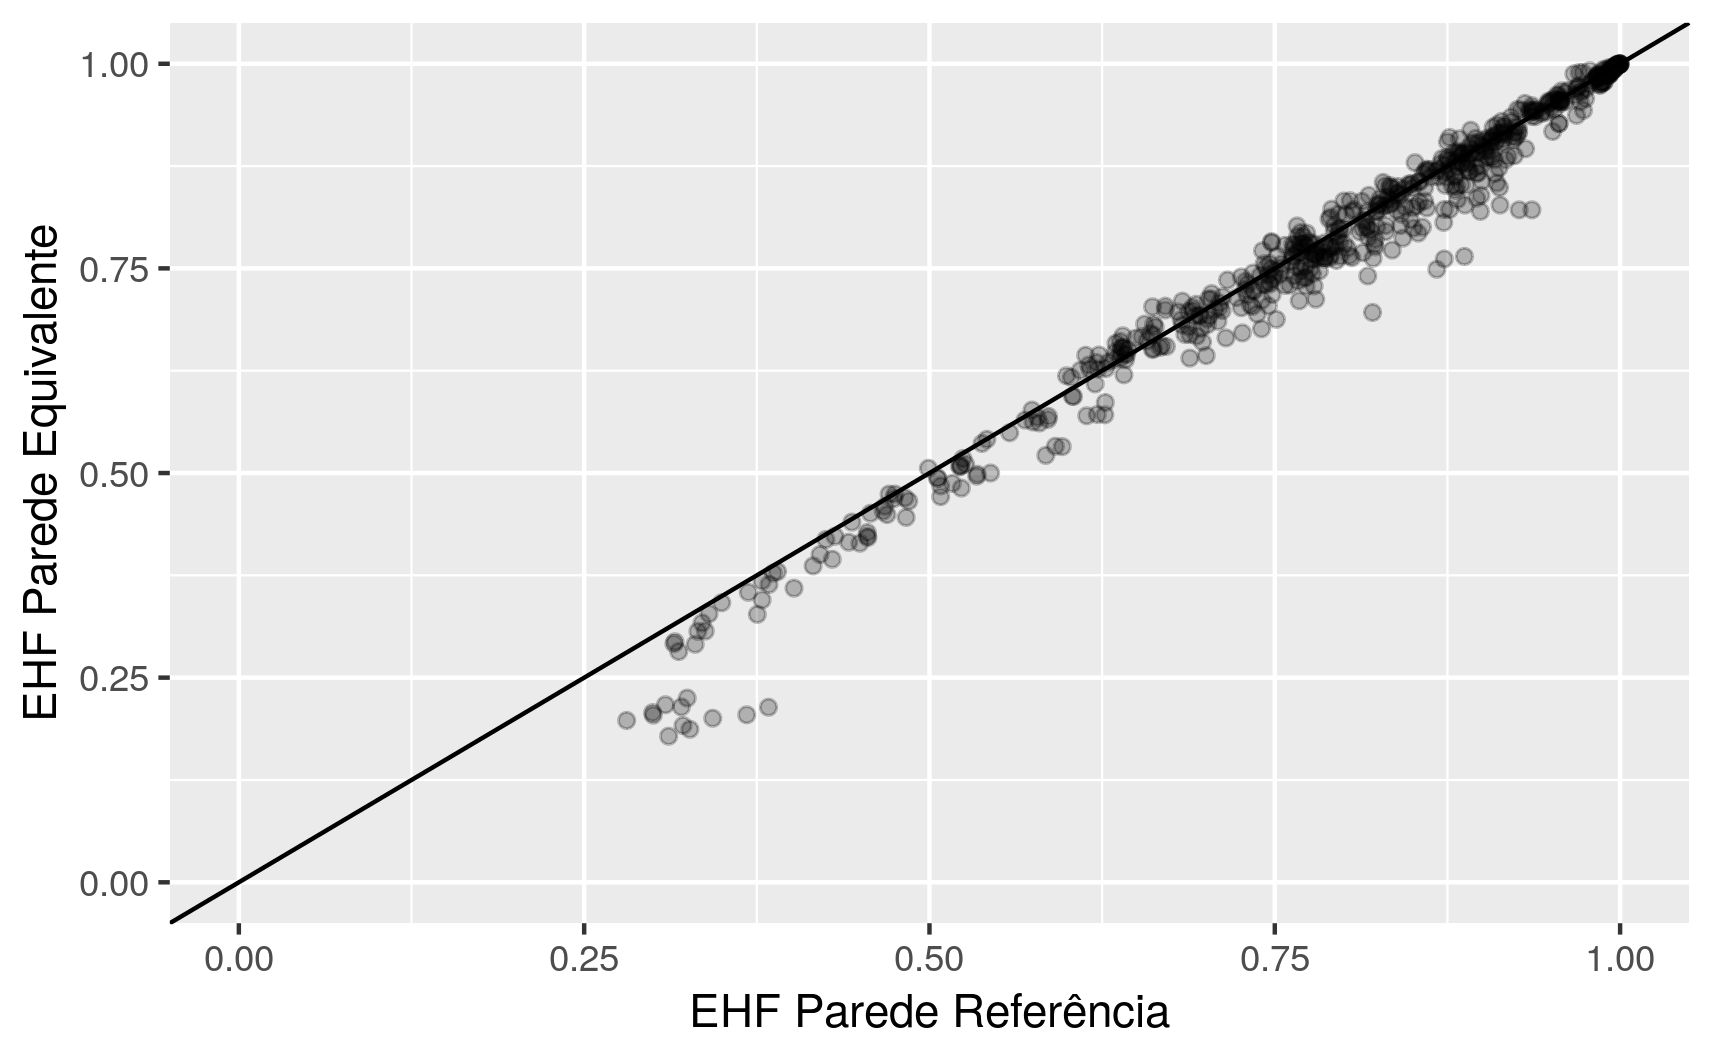
\includegraphics[width=\linewidth]{img/paredeeq_EHF_par2b_scatter.png}
		%		\caption{Comparação entre os valores de \acrshort{cp} das 25 geometrias}
		\begin{center}
			\small{(b) metade do valor da capacidade térmica}\\
%			\phantom{}		
		\end{center}
	\end{minipage}
	\label{fig:par2_scatter}
\end{figure}

O caso com as maiores diferenças no \acrshort{ehf} foi para uma edificação em contato com o solo, com cobertura exposta, e um fator de abertura da janela igual a 0,23.
Apesar das diferenças nos resultados, o uso da parede equivalente facilita a parametrização da transmitância térmica e da capacidade térmica. Por esse motivo, considerou-se as diferenças pouco significativas, e a parede equivalente foi adotada para simplificar as simulações.

\subsection{Condição de contorno das paredes adjacentes à edificação}

A simplificação das simulações adotando-se apenas uma zona térmica foi avaliada para duas condições de contorno. Os resultados mostram que a maneira mais adequada de representar as paredes adjacentes à circulação da edificação é considerando-as como adiabáticas (sem trocas de calor pela superfície).
Considerar as paredes adjacentes à circulação como \textit{Outdoors} (voltada para o lado externo, sem incidência de radiação solar ou vento), faz com que os resultados do \acrshort{ehf} sejam subestimados em 0,0868 em média, como \acrshort{ae95} igual a 0,1865 (Figura \ref{fig:szout}a).
Os resultados das simulações considerando-se as paredes voltadas para o corredor como adiabáticas subestimaram o \acrshort{ehf} em 0,0051 na média, como \acrshort{ae95} igual a 0,0804 (Figura \ref{fig:szout}b).

\begin{figure}[h]
	\caption{Comparação entre os resultados de EHF para diferentes condições de contorno das paredes}
	\begin{minipage}{.5\textwidth}
		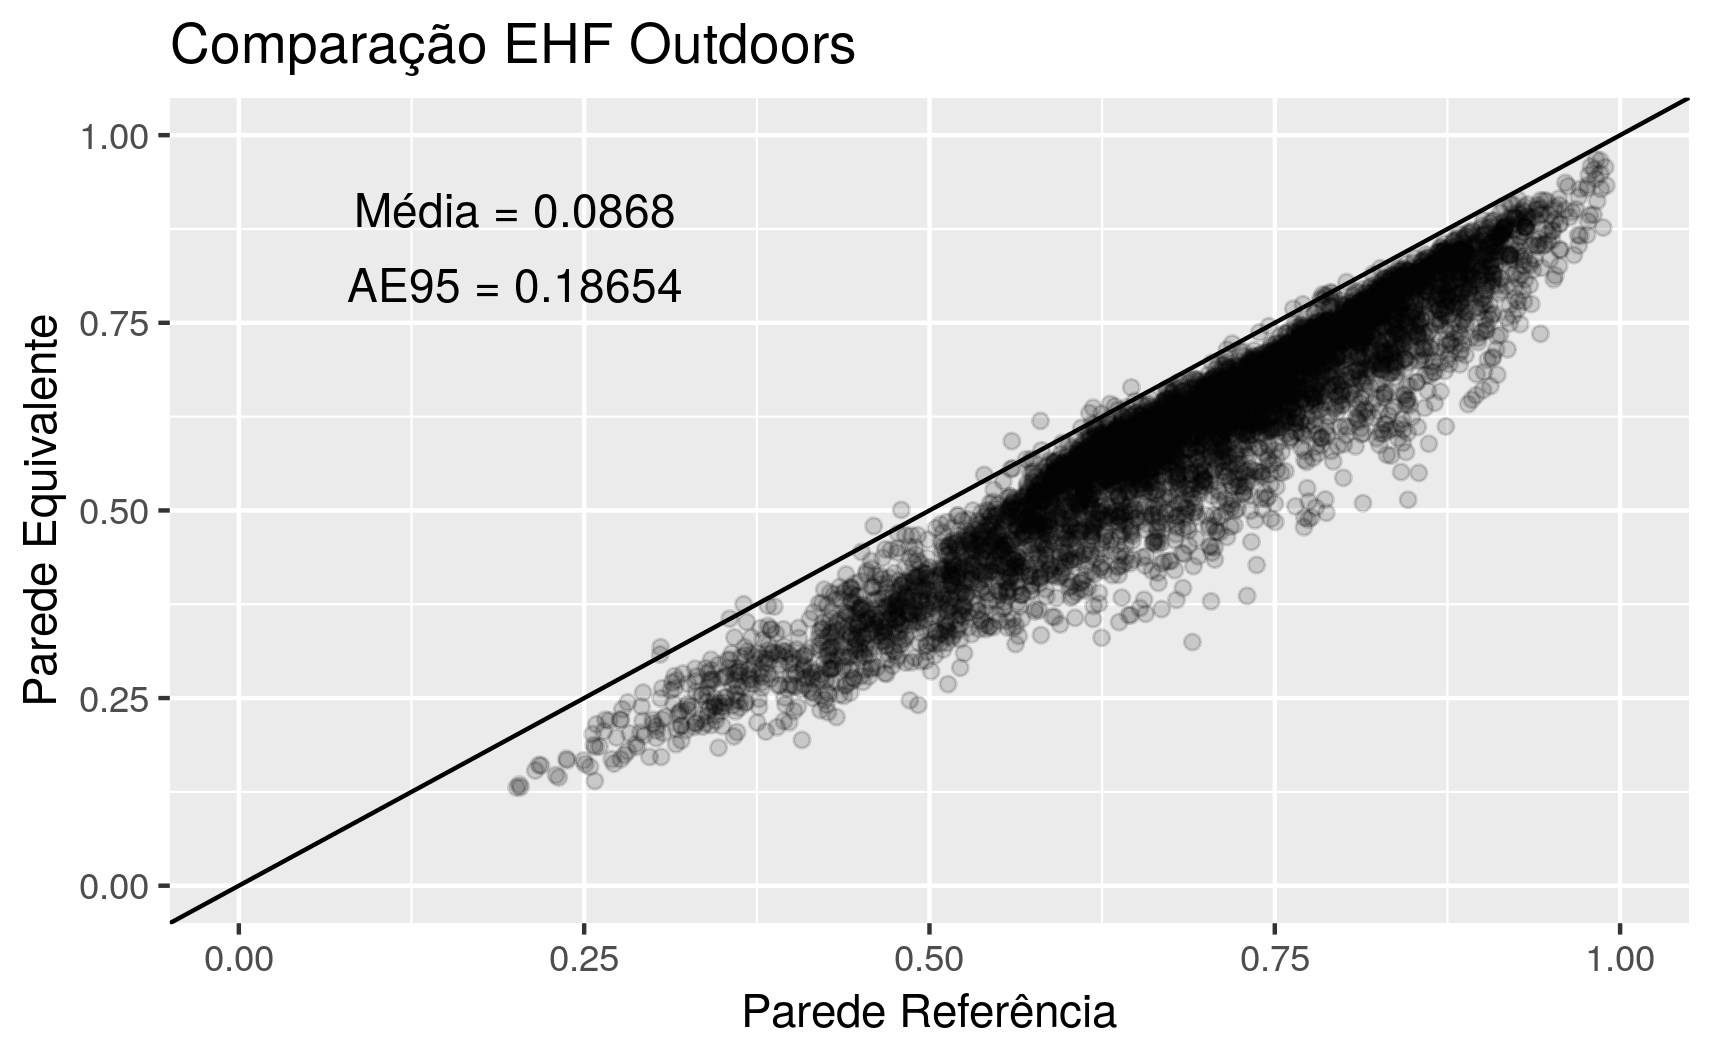
\includegraphics[width=\linewidth]{img/szout_EHF_scatter.png}
		\begin{center}
			\small{(a) \textit{Outdoors}}
		\end{center}
	\end{minipage}%
	\begin{minipage}{.5\textwidth}
		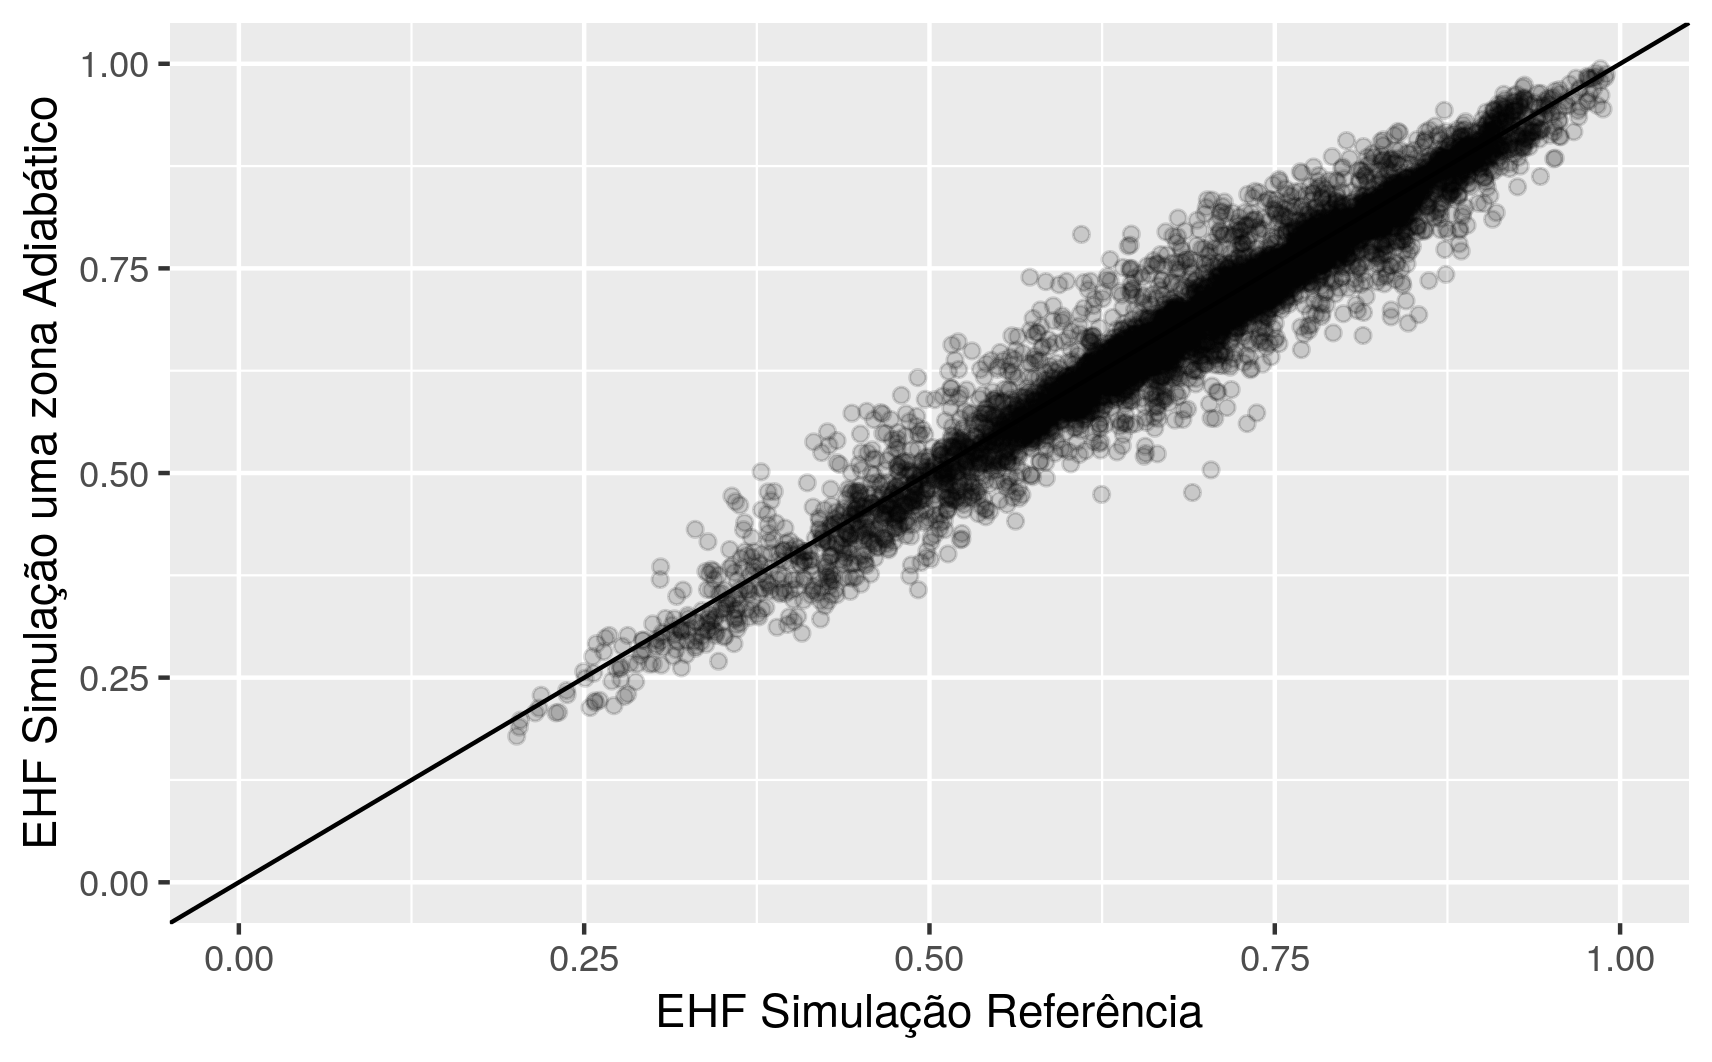
\includegraphics[width=\linewidth]{img/szadi_EHF_scatter.png}
		\begin{center}
			\small{(b) Adiabática}\\
			%			\phantom{}		
		\end{center}
	\end{minipage}
	\label{fig:szout}
\end{figure}

%\begin{figure}[H]
%	\centering
%	\caption{Comparação entre os resultados de EHF para parede \textit{Outdoors}}
%	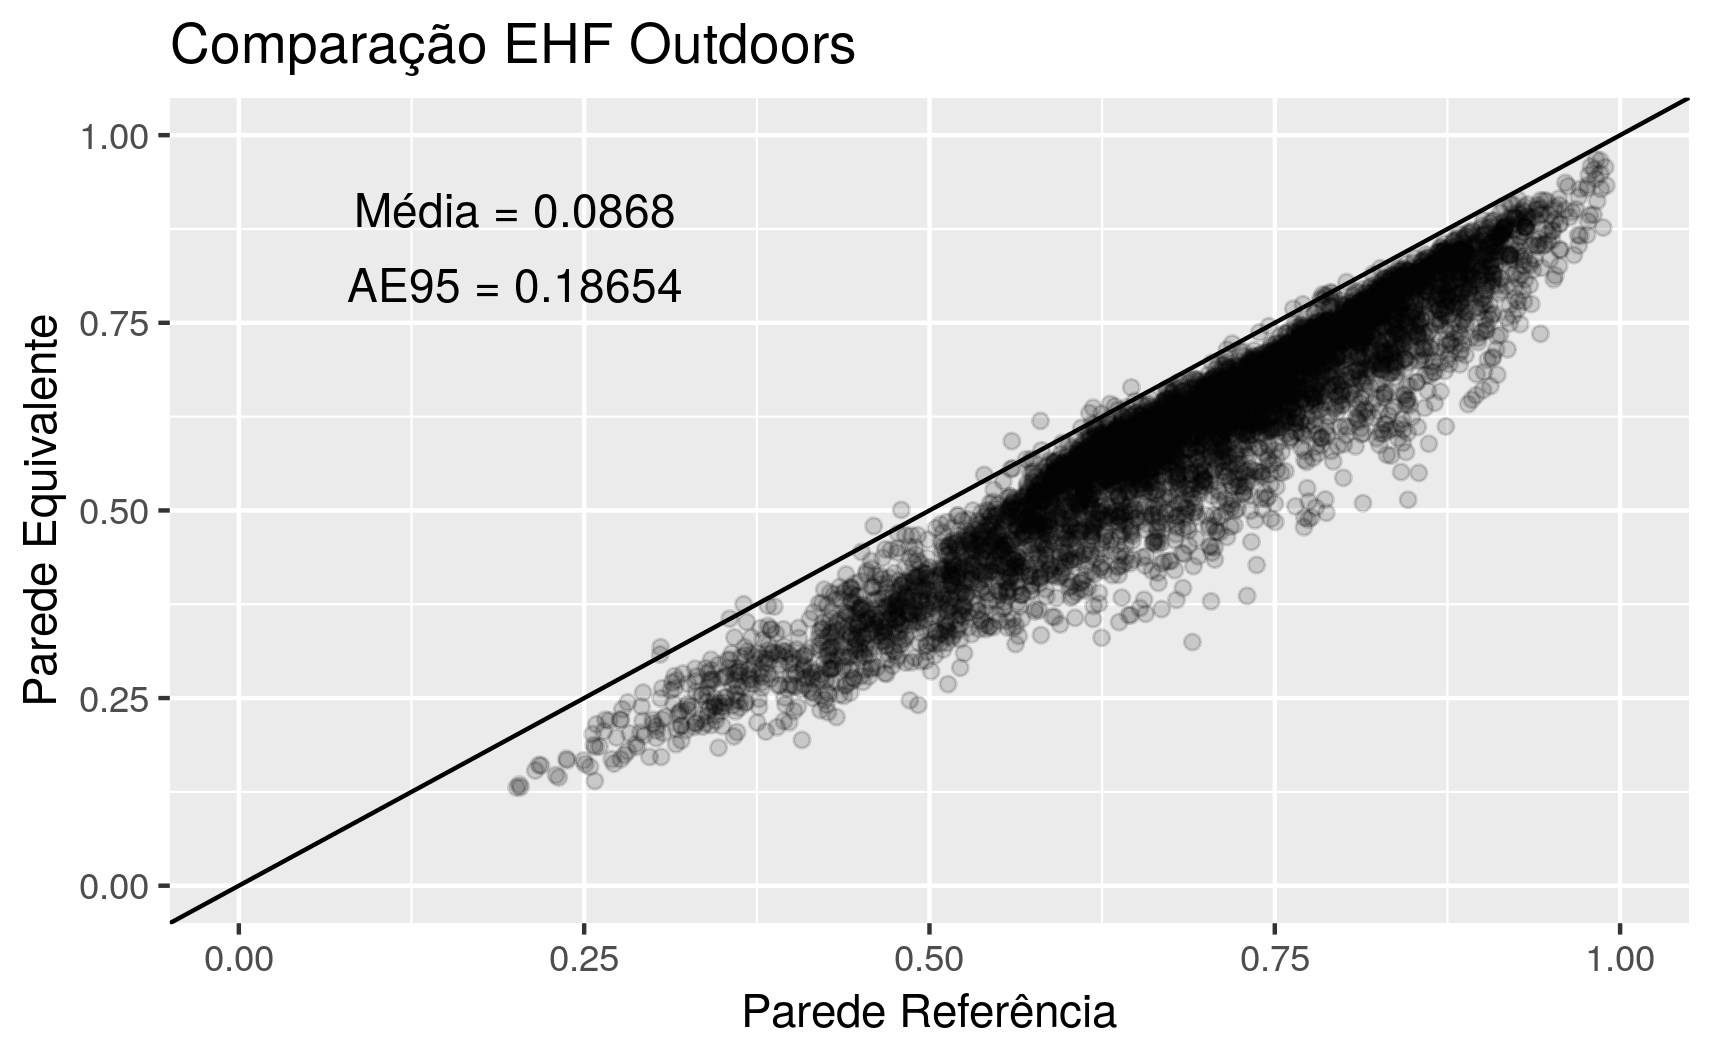
\includegraphics[width=1\linewidth]{img/szout_EHF_scatter.png}
%	\label{fig:szout_EHF}
%	%			\begin{flushleft}
%	%				Fonte: o autor.
%	%			\end{flushleft}
%\end{figure}

%\begin{figure}[H]
%	\centering
%	\caption{Comparação entre os resultados de EHF para parede adiabática}
%	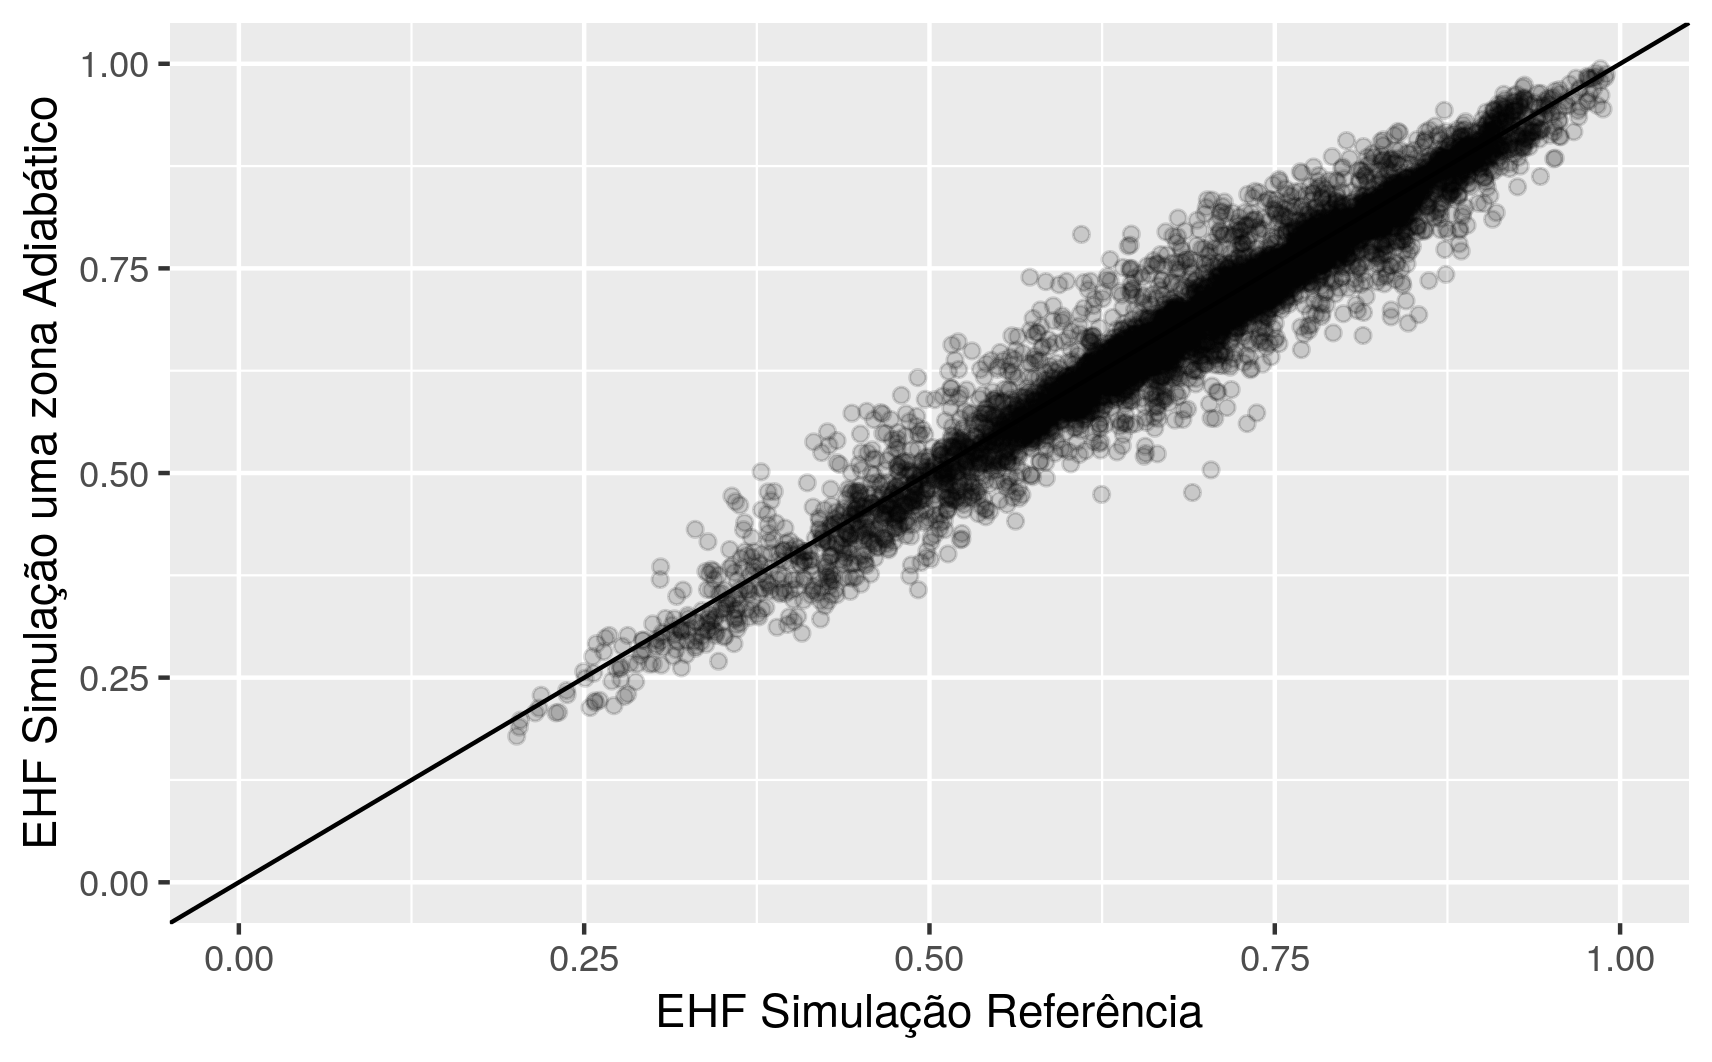
\includegraphics[width=1\linewidth]{img/szadi_EHF_scatter.png}
%	\label{fig:szadi_EHF}
%	%			\begin{flushleft}
%	%				Fonte: o autor.
%	%			\end{flushleft}
%\end{figure}

A partir dos resultados obtidos, definiu-se as paredes voltadas para a circulação como adiabáticas no desenvolvimento das simulações simplificadas.

\subsection{Modelagem da ventilação natural na simulação simplificada}

Nesta etapa do trabalho, as simulações foram conduzidas para se obter duas respostas:
(1) se é adequado o uso do \acrfull{cpeq} para ser associado à porta da zona térmica; (2) qual deveria ser o coeficiente de vazão mássica de ar adotado para o objeto \textit{AirflowNetwork:MultiZone:Surface:Crack}.

Para analisar simultaneamente o desempenho do $Cp_{eq}$ e dos coeficientes de vazão mássica de ar, o gráfico da Figura \ref{fig:pareto} foi gerado, observando-se as raízes dos erros médios quadráticos (\acrshort{rmse}).
É possível observar que as simulações desenvolvidas utilizando-se o $Cp_{eq}$ obtiveram resultados com \acrshort{rmse} menores do que as simulações desenvolvidas utilizando-se o \acrshort{cp} obtido diretamente pelo \acrlong{ma}.
Para a definir o coeficiente de vazão mássica de ar, levou-se em conta, inicialmente, os erros relacionados ao \acrshort{ach}.
No entanto, foi identificada uma fronteira de Pareto entre os erros analisados, que mostra como a busca por menores erros de \acrshort{ach} aumenta os erros relacionados ao \acrshort{ehf}.
O resultado dessa análise pode ser atribuída ao fato de que as diferenças maiores nas trocas de ar anulem erros relacionados à definição das paredes adjacentes à edificação como adiabáticas, ou porque os maiores erros relacionados à médias anuais do \acrshort{ach} sejam em casos onde as diferenças nas trocas de ar não sejam relevantes para alterar a temperatura operativa nas zonas térmicas e, consequentemente, o \acrshort{ehf}.

\begin{figure}[h]
	\centering
	\caption{Eficiência de Pareto entre EHF e ACH médio}
	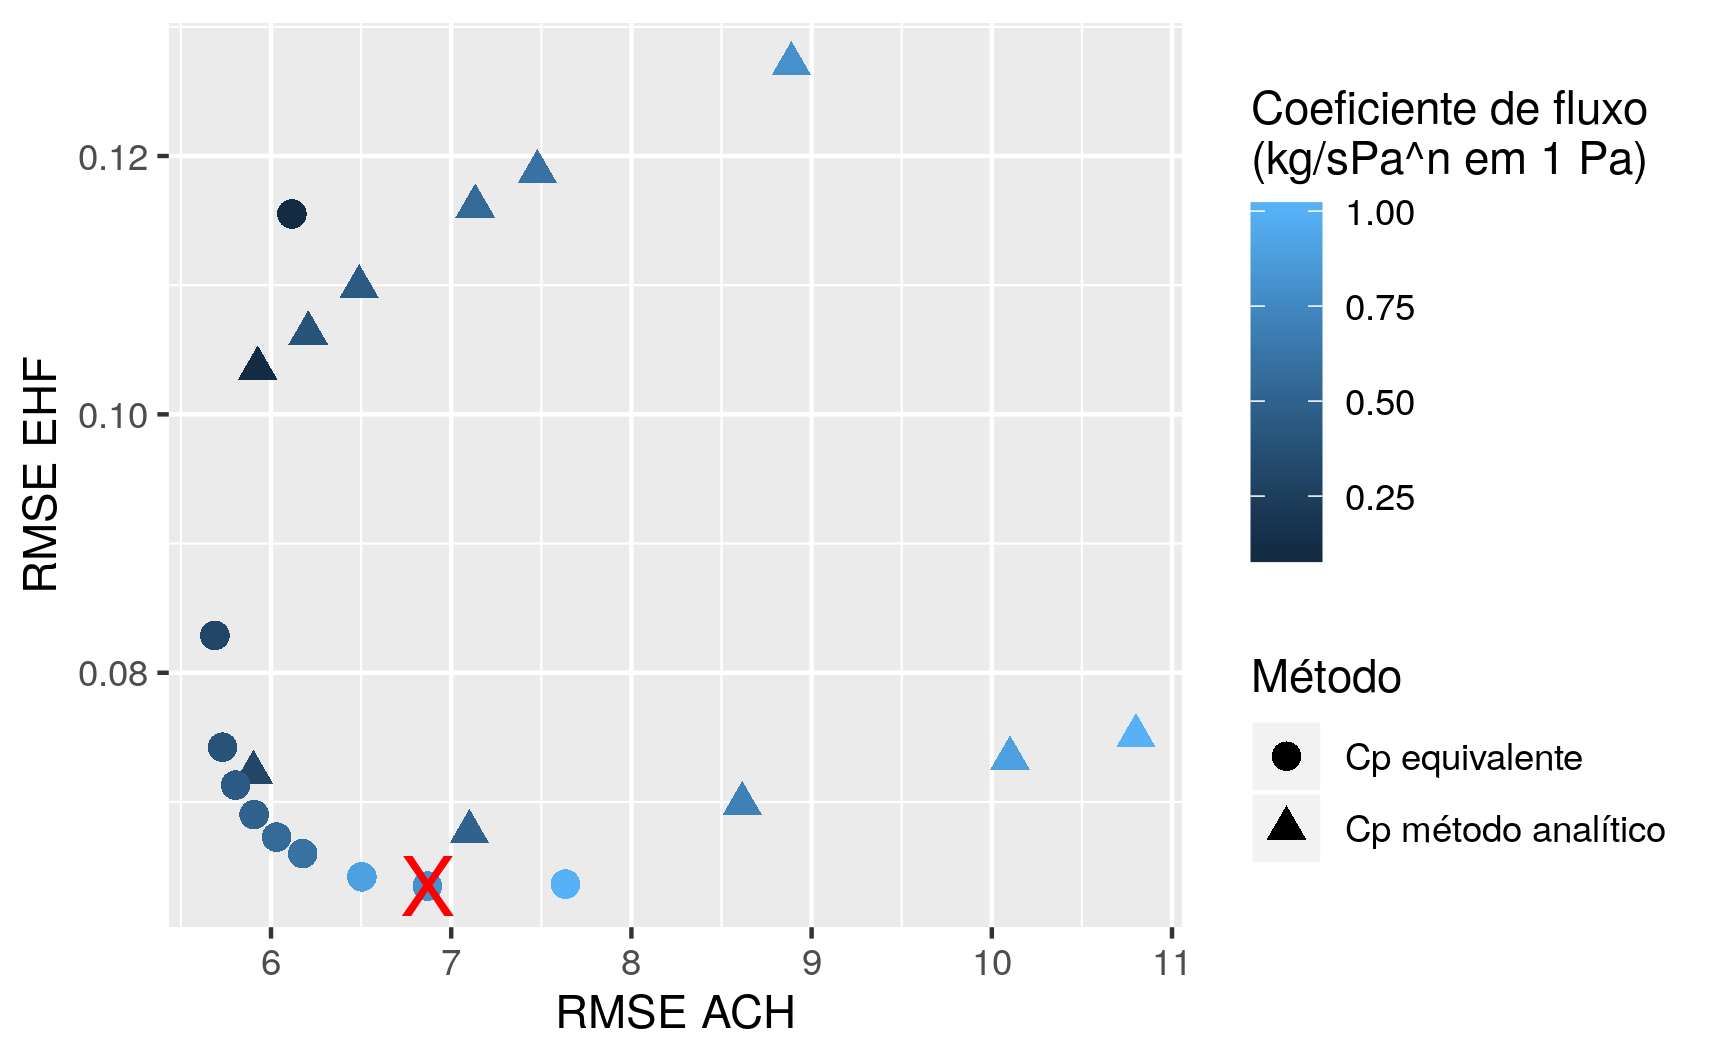
\includegraphics[width=1\linewidth]{img/cpeq_pareto.png}
	\label{fig:pareto}
	%			\begin{flushleft}
	%				Fonte: o autor.
	%			\end{flushleft}
\end{figure}

Como o desenvolvimento das simulações é voltado para obter a maior exatidão possível para os resultados de \acrshort{ehf}, optou-se por definir o coeficiente de vazão mássica de ar com valor igual a 0,8 kg/sPa$^n$ em 1 Pa, pois as simulações desenvolvidas utilizando-se este valor estão na fronteira de Pareto, e resultaram nos menores erros de \acrshort{ehf}.
Na Figura \ref{fig:pareto}, o ponto do coeficiente de vazão mássica de ar com valor a 0,8 kg/sPa$^n$ em 1 Pa está destacado com um "X".
A Figura \ref{fig:crack08} apresenta a comparação dos resultados de \acrshort{ach} e \acrshort{ehf} obtidos pelas simulações detalhadas, comparados aos resultados obtidos pela simulação simplificada, utilizando-se o coeficiente de vazão mássica de ar adotado, com valor igual 0,8 kg/sPa$^n$ em 1 Pa.

\begin{figure}[h]
	\caption{Comparação entre os resultados de ACH e EHF para coeficiente de vazão mássica de ar com valor igual 0,8 kg/sPa$^n$ em 1 Pa}
	\begin{minipage}{.5\textwidth}
		\centering
		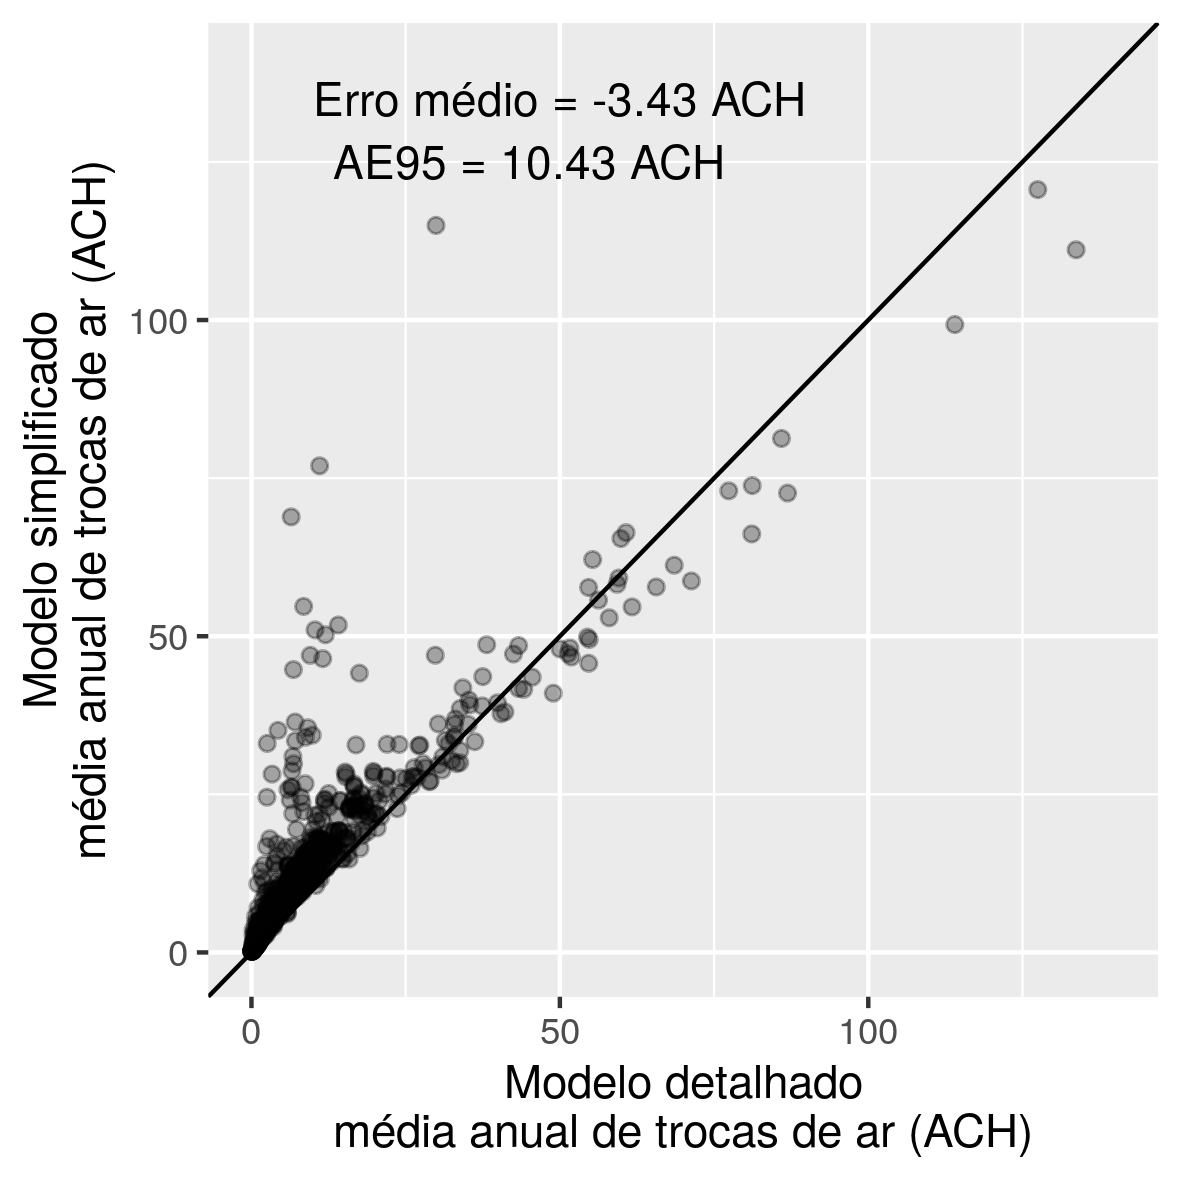
\includegraphics[width=1\linewidth]{img/cpeq_COM_80.png}
		\begin{center}
			\small{(a) comparação do \acrshort{ach}}
		\end{center}
	\end{minipage}%
	\begin{minipage}{.5\textwidth}
		\centering
		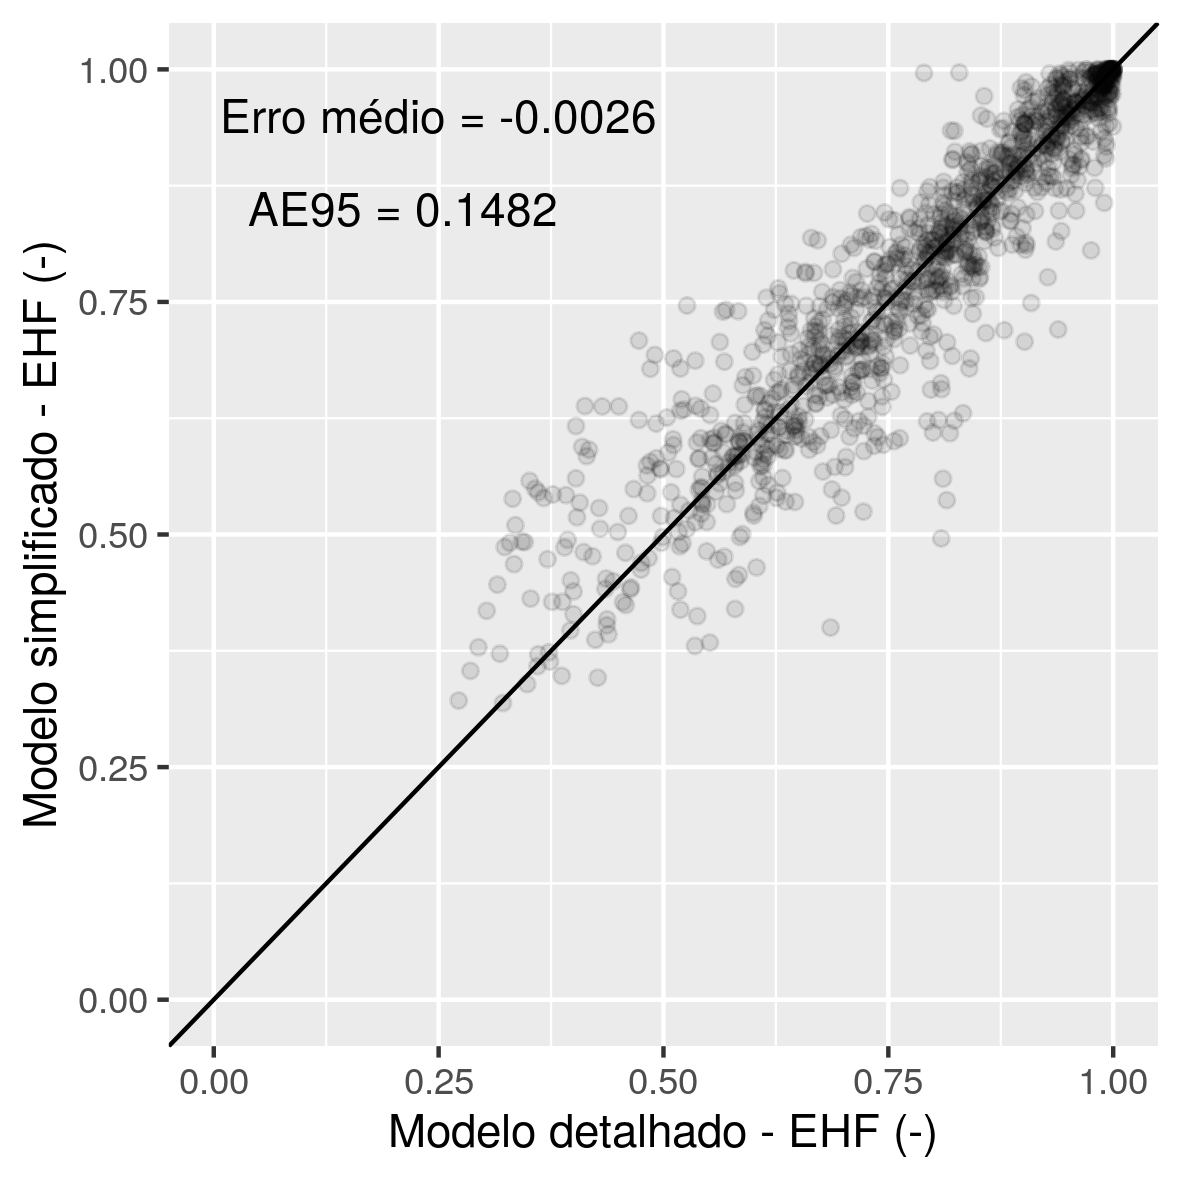
\includegraphics[width=1\linewidth]{img/cpeq_COM_80EHF.png}
		\begin{center}
			\small{(b) comparação do \acrshort{ehf}}
		\end{center}
	\end{minipage}
	\label{fig:crack08}
\end{figure}

\newpage

\section{Análise de sensibilidade}

As análises de sensibilidade (\acrshort{as}) foram aplicadas a partir de 155.648 simulações termoenergéticas, a partir das quais se obteve valores de \acrshort{ehf} entre 0,01 e 1,00 (Figura \ref{fig:sobol_EHF}).
A ausência de resultados de \acrshort{ehf} iguais a zero indica que, para o clima da cidade de São Paulo, o uso exclusivo de \acrshort{vn} como estratégia de resfriamento para edifícios de escritórios não é suficiente para garantir conforto térmico em todas as horas de ocupação ao longo do ano. Entretanto, a variabilidade dos resultados obtidos evidencia como o potencial de conforto térmico depende da configuração adequada dos parâmetros de projeto.

\begin{figure}[h]
	\centering
	\caption{Valores de EHF obtidos no desenvolvimento das análises de sensibilidade}
	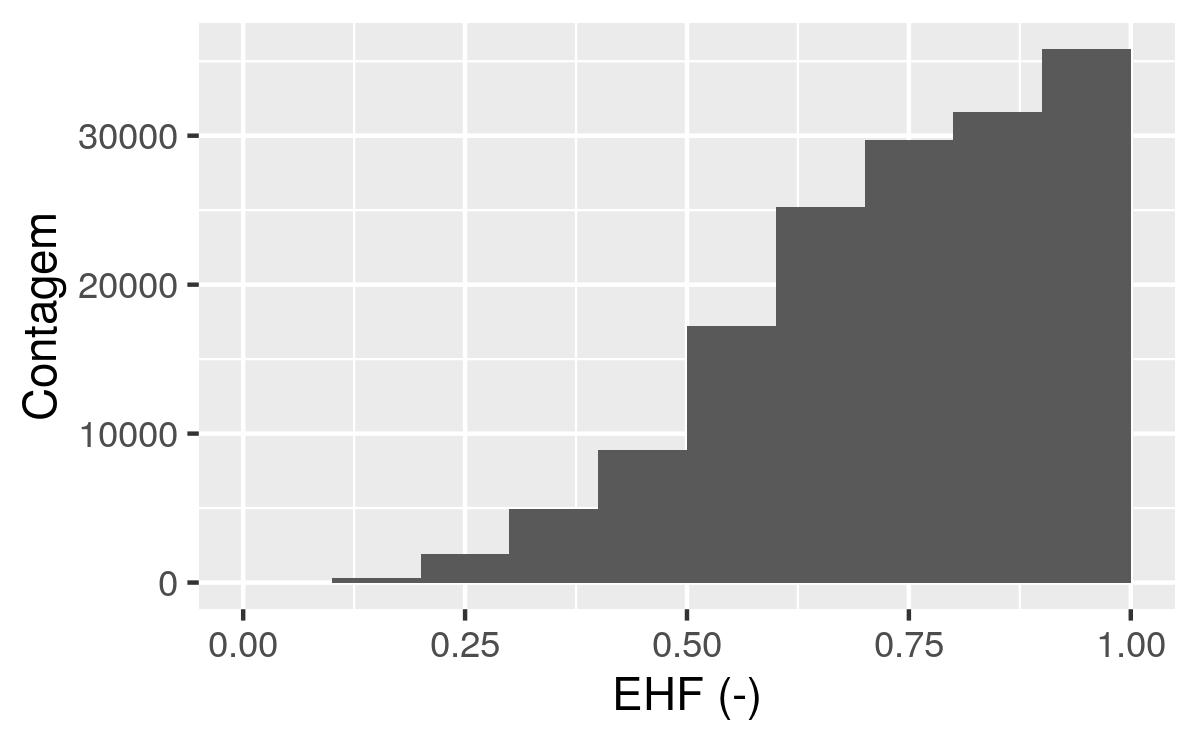
\includegraphics[width=.7\linewidth]{img/sobol_EHF.png}
	\label{fig:sobol_EHF}
	%			\begin{flushleft}
	%				Fonte: o autor.
	%			\end{flushleft}
\end{figure}

\newpage
As Figuras \ref{fig:as_ach}, \ref{fig:as_temp} e \ref{fig:as_ehf} apresentam os resultados das análises de sensibilidade (\acrshort{as}) para efeitos de primeira ordem e efeitos totais, relacionados ao \acrshort{ehf}, às temperaturas operativas das zonas, e ao \acrshort{ehf}. Os índices apresentados são proporcionais às influências entre os dados de entrada e saída.

\begin{figure}[H]
	\centering
	\caption{Análise de sensibilidade de Sobol dos efeitos de primeira ordem e efeitos totais nas médias anuais de ACH}
	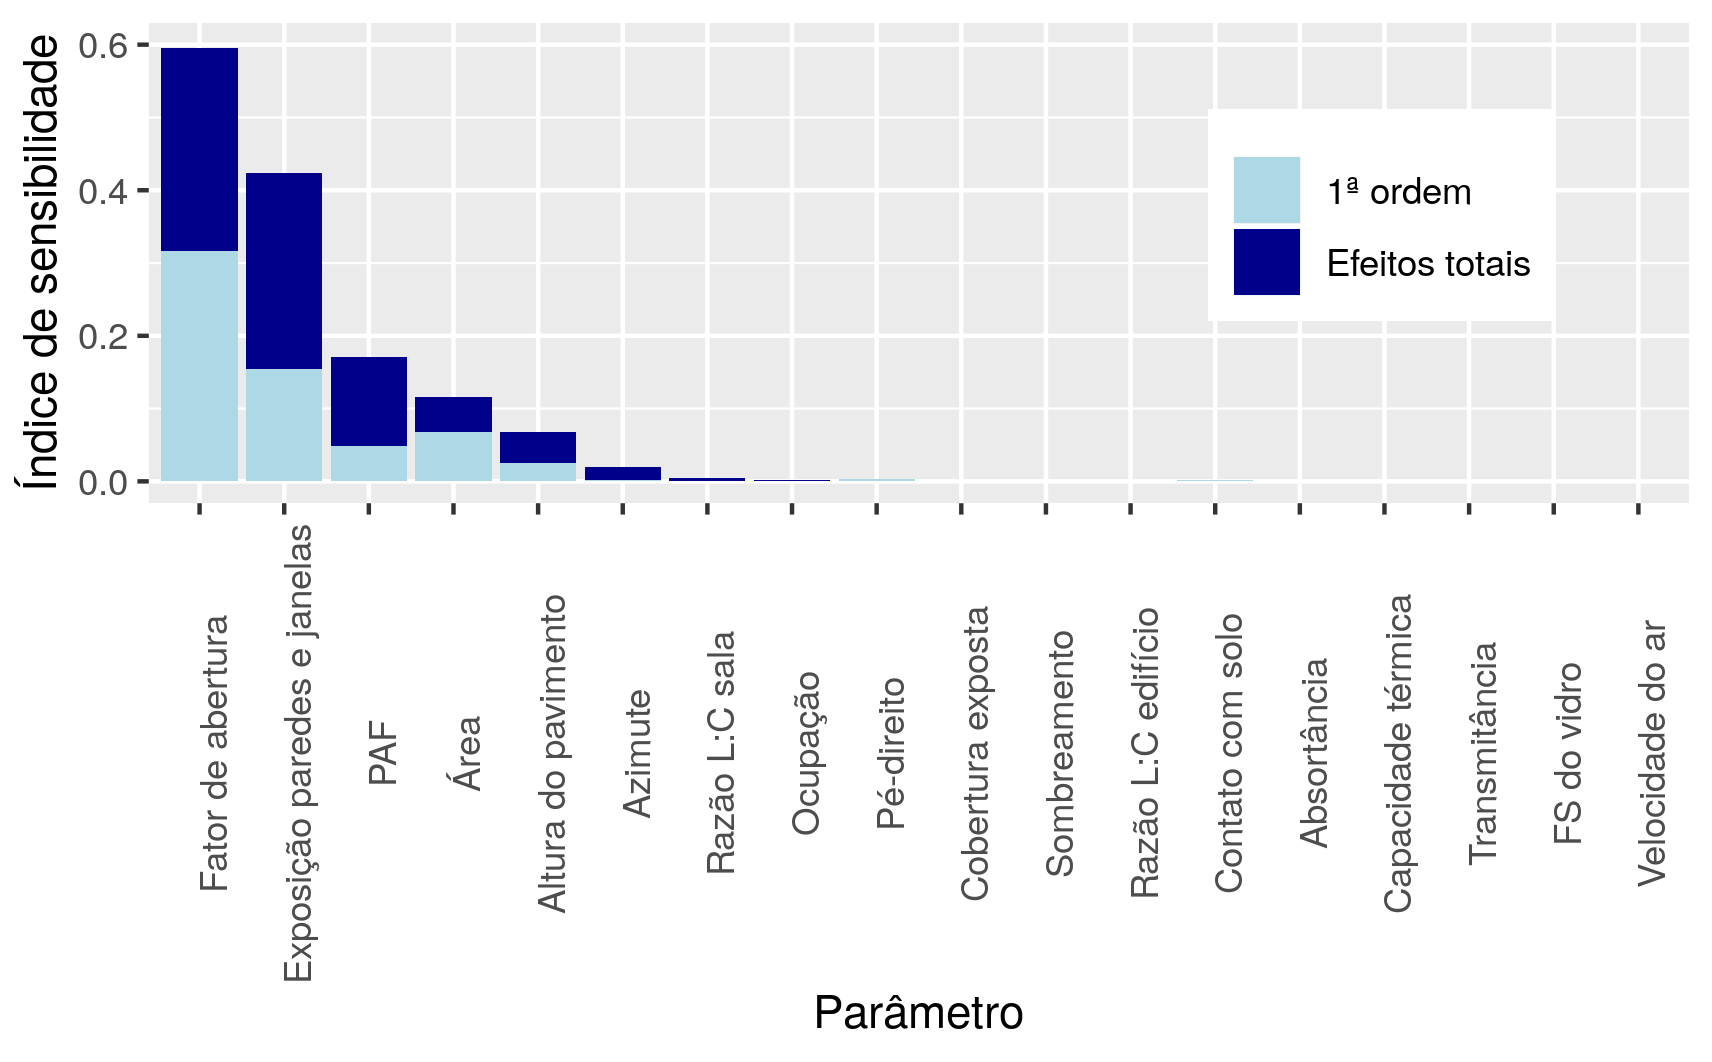
\includegraphics[width=\sasize\linewidth]{img/as_ach.png}
	\label{fig:as_ach}
	%			\begin{flushleft}
	%				Fonte: o autor.
	%			\end{flushleft}
\end{figure}

Os parâmetros mais influentes no \acrshort{ach}, como esperado, são aqueles relacionados às aberturas da zona. 
O primeiro parâmetro de maior influência é o fator de abertura das janelas, seguido do parâmetro relacionado à exposição das paredes e à presença de \acrshort{vn} cruzada ou unilateral. 
A área da zona  térmica tem influência significativa, pois o cálculo das trocas de ar leva em conta o volume de ar na zona, que é diretamente relacionado à sua área. 
A altura do pavimento é determinante nos resultados do \acrshort{ach}, pois a velocidade do vento no EnergyPlus é calculada em função da altura da zona.
A orientação da zona (azimute) não tem uma influência significativa de primeira ordem. No entanto, percebe-se uma influência mais significativa considerando-se os efeitos totais. 
O azimute é determinante para a definição dos coeficientes de pressão sobre as fachadas da edificação. Por isso, a influência deste parâmetro nos resultados das simulações depende de outros parâmetros, relacionados ao posicionamento e às áreas das aberturas na zona.
A velocidade do ar não influencia os resultados relacionados ao \acrshort{ach}, pois é considerada somente após o término das simulações, ao se calcular o \acrshort{ach}.
A \acrshort{as} apresentou interações de segunda ordem significativas entre o fator de abertura das janelas e a presença de \acrshort{vn} cruzada ou unilateral, com um índice de sensibilidade igual a 0,121.
Contudo, o parâmetro com maiores interações de segunda ordem relacionados ao \acrshort{ach} foi o \acrshort{paf}, com a soma dos índices de segunda ordem igual a 0,300.

\begin{figure}[H]
	\centering
	\caption{Análise de sensibilidade de Sobol dos efeitos de primeira ordem e efeitos totais nas temperaturas operativas}
	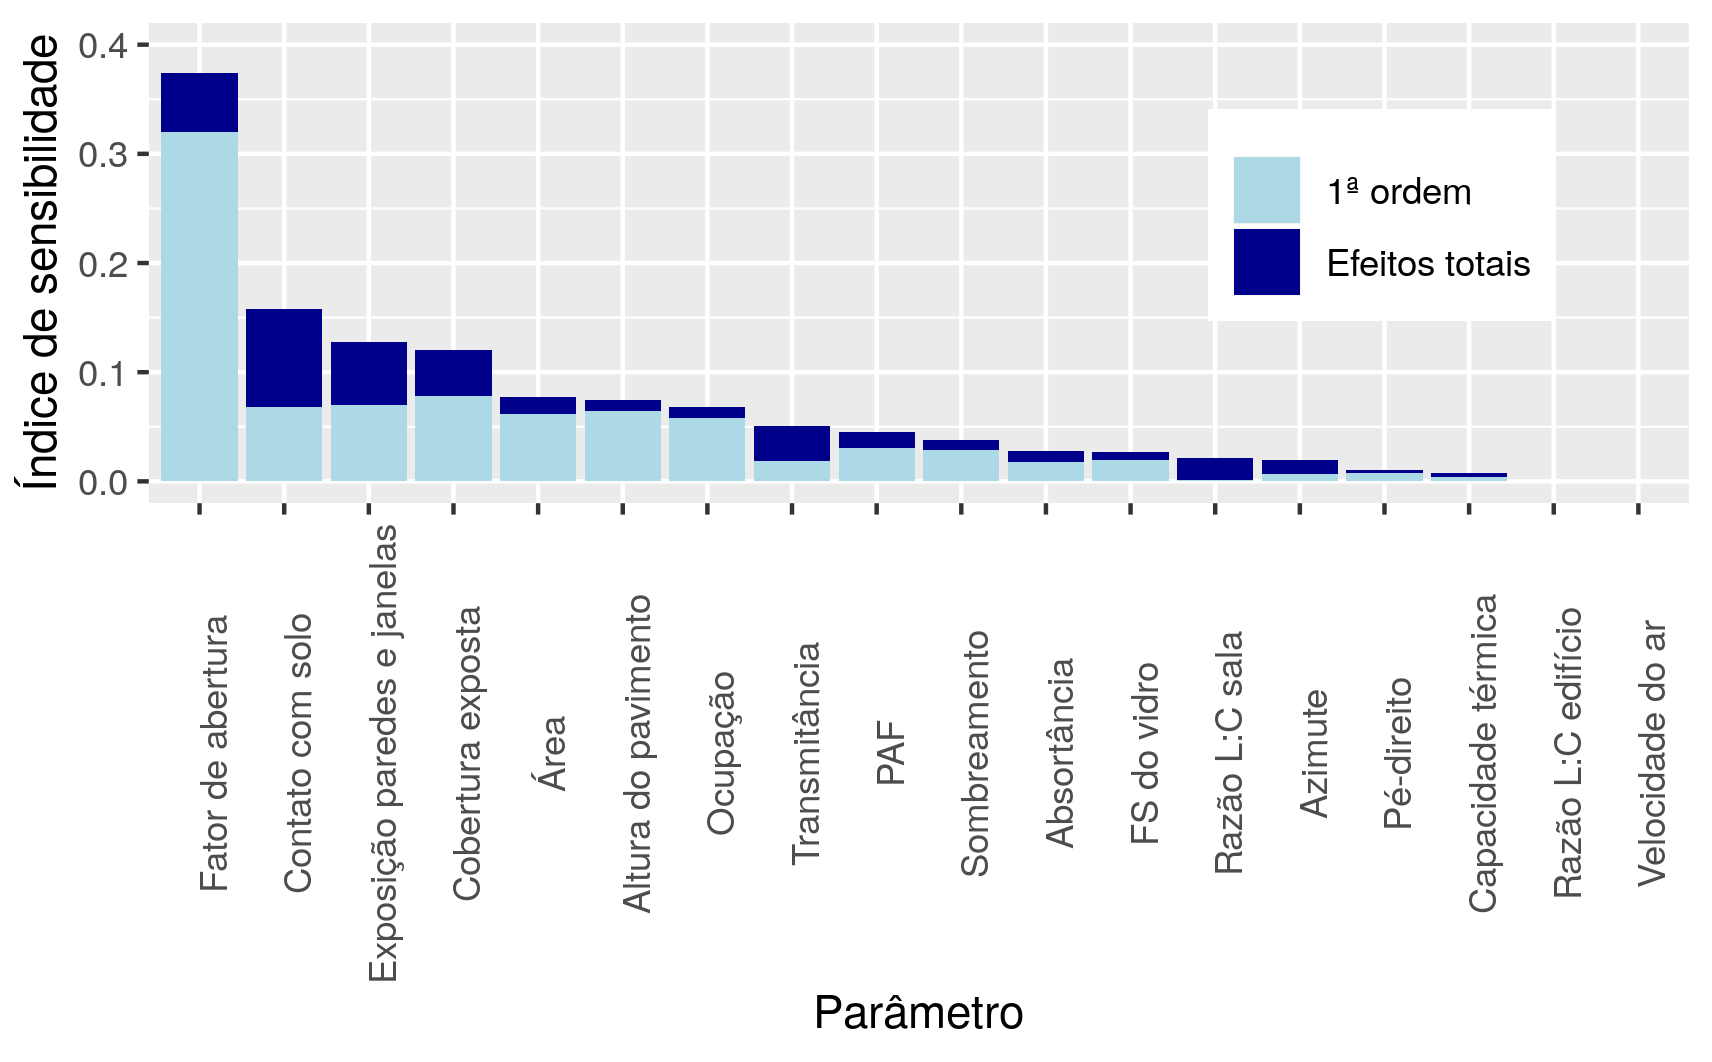
\includegraphics[width=\sasize\linewidth]{img/as_temp.png}
	\label{fig:as_temp}
	%			\begin{flushleft}
	%				Fonte: o autor.
	%			\end{flushleft}
\end{figure}

\begin{figure}[H]
	\centering
	\caption{Análise de sensibilidade de Sobol dos efeitos de primeira ordem e efeitos totais no EHF}
	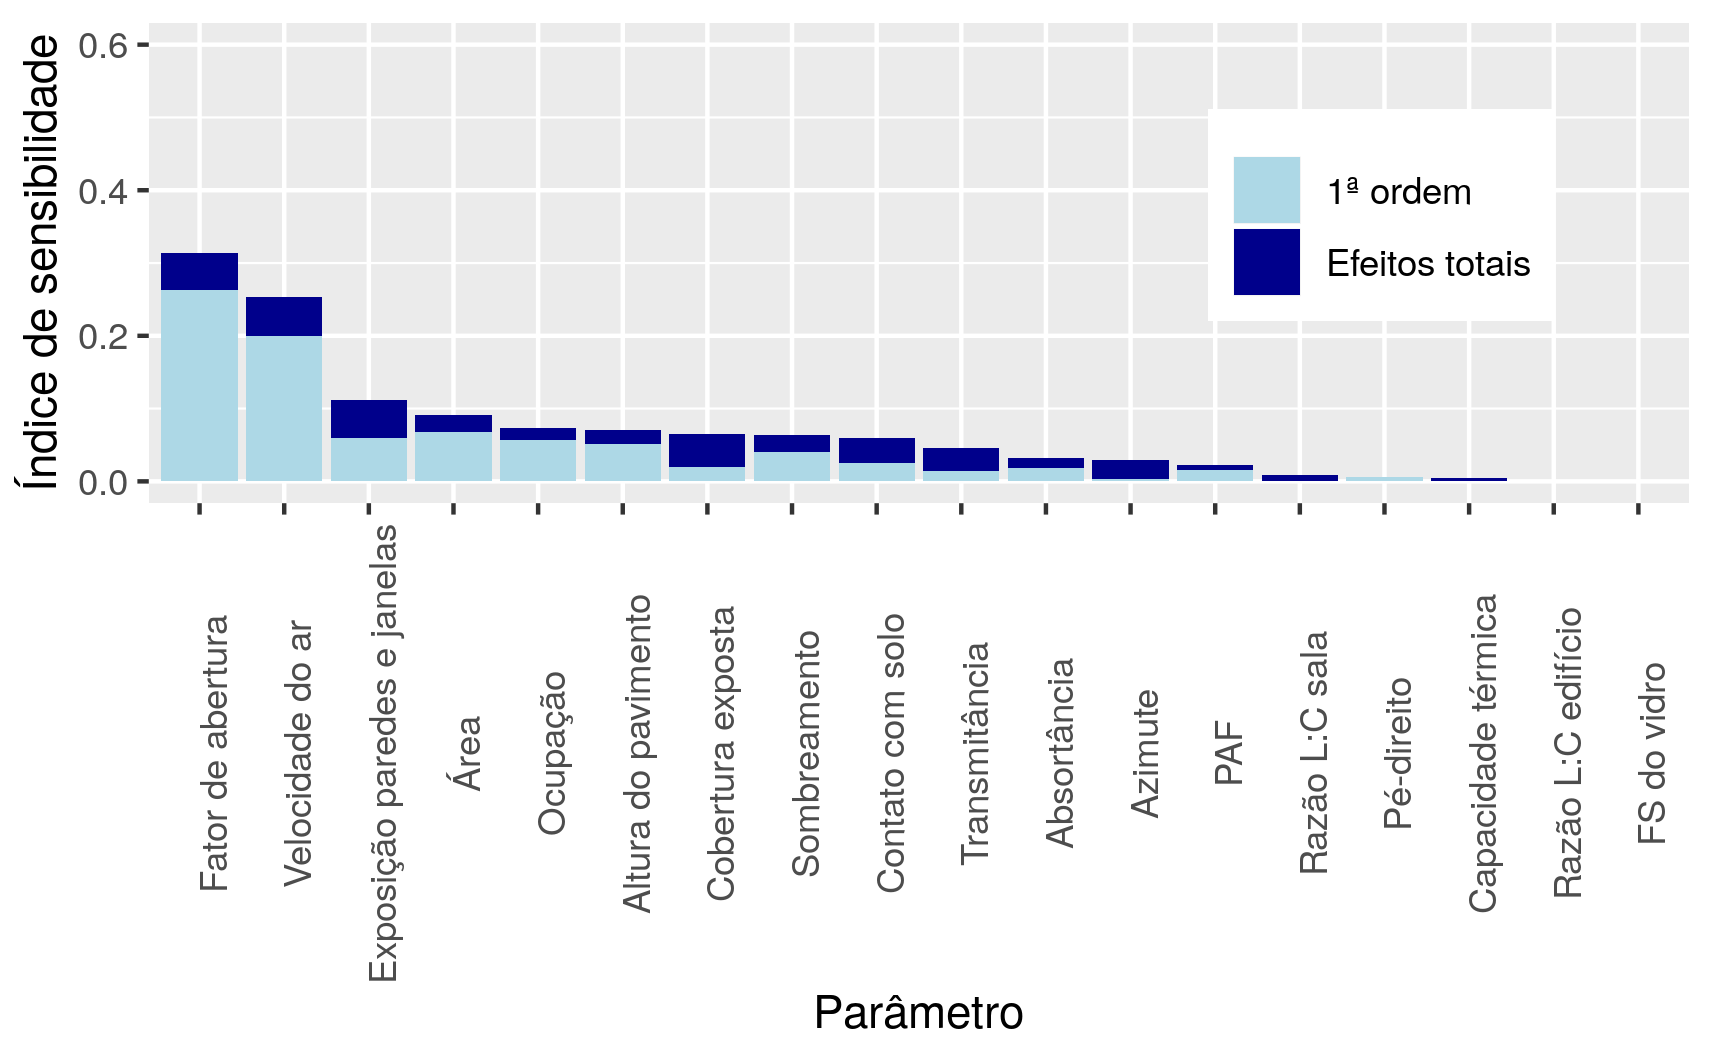
\includegraphics[width=\sasize\linewidth]{img/as_ehf.png}
	\label{fig:as_ehf}
	%			\begin{flushleft}
	%				Fonte: o autor.
	%			\end{flushleft}
\end{figure}

As análises relacionadas à temperatura operativa e ao \acrshort{ehf} indicam relevância dos parâmetros relacionados à \acrshort{vn}. Para ambas as análises, o parâmetro mais influente foi o fator de abertura da janela, enquanto o parâmetro relacionado à exposição das paredes e à presença de \acrshort{vn} cruzada ou unilateral foi o terceiro mais influente. 
O contato com o solo apresentou-se como o segundo parâmetro mais influente nas médias anuais de temperatura operativa, considerando-se os esfeitos totais. No entanto, a influência deste parâmetro não é tão significativa no \acrshort{ehf}. Isso indica que a influência do contato com o solo nas temperaturas operativas das zonas é mais significativa em faixas de temperatura que não interferem no cálculo do \acrshort{ehf}, ou seja, consideravelmente acima ou abaixo dos limites superiores de aceitabilidade estabelecidos pelo método de conforto adaptativo.
Observa-se que os efeitos totais entre o segundo (contato com o solo) e o quarto (exposição da cobertura) índice de sensibilidade com valores mais altos na \acrshort{as} relacionada à média anual da temperatura operativa são expressivos.
A transmitância das paredes, o azimute, e a razão entre a largura e o comprimento da sala também apresentam efeitos totais relevantes, apesar dos baixos índices de sensibilidade para primeira ordem. Isso indica que há interações significativas entre esses parâmetros e os demais.

O movimento do ar apresenta-se como o segundo parâmetro mais influente nos resultados de \acrshort{ehf}, o que indica um grande potencial de uso de ventiladores na busca por conforto térmico nos ambientes. 
A área da zona e a densidade de ocupação apresentaram-se mais influentes nos resultados de \acrshort{ehf}, comparando-se aos resultados relacionados às médias anuais de temperatura operativa.
O azimute, apesar de seu índice de sensibilidade baixo para a análise de primeira ordem, apresentou índices de segunda ordem expressivos. As interações de segunda ordem ocorrem relacionadas a parâmetros referentes à \acrshort{vn} e a parâmetros referentes à radiação solar. A soma dos índices de segunda ordem do azimute em relação ao \acrshort{ehf} foi igual a 0,177.  %, como sombreamento e absortância

A complexidade dos fenômenos representados junto às interações entre as diferentes variáveis exige um grande número de casos para reduzir incertezas, pois o método de \acrshort{as} utiliza uma base amostral. Por isso, existe uma incerteza associada aos índices de sensibilidade obtidos nas \acrshort{as} conduzidas, e a soma dos valores dos índices ultrapassa o valor 1. Entretanto, a aplicação da análise de sensibilidade global ofereceu resultados relevantes para o trabalho, com índices de sensibilidade condizentes aos comportamentos físicos representados pelas simulações. 

Baseando-se nos resultados das \acrshort{as}, alguns dos parâmetros não foram considerados para o desenvolvimento do metamodelo. Desconsiderar parâmetros com índices de sensibilidade significativamente baixos possibilita o desenvolvimento de um metamodelo mais simples, com menos dados de entrada e maior precisão nos resultados. Os parâmetros desconsiderados tiveram seus valores fixados, de acordo com a Tabela \ref{table:param_fixed}. O valor do pé-direito foi determinado considerando-se o valor encontrado com mais frequência na base de dados analisada. A capacidade térmica da parede foi estabelecida de acordo com o valor de uma parede de bloco cerâmico de dimensões 14x19x29 cm, e argamassa de 2,5 cm, resultando em um valor de 161 kJ/m$^2$K. No entanto, como as simulações foram desenvolvidos com o modelo de parede equivalente, considerou-se apenas metade do valor da capacidade térmica. Os parâmetros relacionados às proporções entre largura e profundidade das salas e edifícios foram determinados com valor igual a 1. 

\begin{table}[h]		
	\centering
	\caption{Parâmetros com valores constantes}
	\label{table:param_fixed}
	\begin{tabular}{|l |c |}
		\hline
		\textbf{Parâmetro} & Valor fixo \\
		\hline
		Razão entre a menor e maior dimensão do edifício ($-$) & 1 \\
		\hline
		Razão entre a menor e maior dimensão da sala ($-$) & 1 \\
		\hline
		Pé-direito ($m$) & 2,5 \\
		\hline
		Capacidade térmica ($kJ/m^2K$) & 80 \\
		\hline
		%			Fator solar do vidro ($-$) & 0,87 \\
		%			\hline
	\end{tabular}
\end{table}

\newpage

\section{Desenvolvimento do metamodelo}
 
O metamodelo final foi definido com 14 parâmetros:
\begin{itemize}
	\item Fator de abertura das janelas;
	\item Velocidade do ar;
	\item Condição de exposição das paredes e janelas;
	\item Área da sala;
	\item Densidade de ocupação;
	\item Altura do pavimento;
	\item Exposição da cobertura;
	\item Sombreamento horizontal;
	\item Contato com o solo;
	\item Transmitância das paredes;
	\item Absortância das paredes;
	\item Fator solar do vidro;
	\item Azimute da sala;
	\item \Acrlong{paf}.
\end{itemize}

As 100.000 simulações termoenergéticas foram desenvolvidas para o treinamento da rede neural artificial (\acrshort{ann}) a partir de combinações entre os parâmetros definidos.
Os parâmetros variaram na mesma faixa de valores estabelecida na Seção \ref{section:parametrosdeentrada}. O ângulo do azimute da sala é determinado considerando-se o eixo entre a parede voltada para a circulação e a parede oposta à circulação.
O contato com o solo e a exposição da cobertura foram definidas como variáveis binárias, com o valor zero correspondendo à superfície adiabática, e 1 correspondendo à exposição.
O parâmetro que representa a condição de exposição das paredes e janelas não foi representado com valores numéricos, e sim como uma variável de fatores, com cinco opções de exposição. Além das três opções apresentadas na Figura \ref{fig:exp_sz}, considerou-se também as exposições espelhadas. 	
Os demais parâmetros foram normalizados com valores entre -1 e 1.

\begin{figure}[h]
	\centering
	\caption{Condição de exposição das paredes e janelas}
	\includegraphics[width=.5\linewidth]{img/wallexposition2.png}
	\label{fig:exp_sz}
	%			\begin{flushleft}
	%				Fonte: o autor.
	%			\end{flushleft}
\end{figure}

O modelo de \acrshort{ann} final foi definido com duas camadas, umas de 50 nós, e a outra com 20. 
O algorítimo de otimização que obteve o melhor desempenho foi o \textit{Adagrad's Optimizer}, disponibilizado pela biblioteca \textit{TensorFlow} \cite{tensorflow2015}, com uma taxa de aprendizagem igual a 0,05. O treinamento foi interrompido após 150.000 iterações. Neste momento, os erros de obtidos para as estimativas da amostra de validação pararam de baixar, e continuar o processo poderia causar o um sobreajuste do metamodelo em relação à amostra de treinamento.

A Figura \ref{fig:ann_validation} apresenta um gráfico de pontos comparando os resultados de \acrshort{ehf} obtidos para as simulações e para as estimativas da \acrshort{ann}, a partir da base de dados desenvolvida para a validação do metamodelo. A base de dados para a validação (Figura \ref{fig:ann_validation}a) teve apenas os parâmetros incluídos no treinamento da \acrshort{ann} variados. 
O erro absoluto médio do \acrshort{ehf} para os casos de validação foi 0,0091, com o \acrshort{ae95} igual a 0,0244.
Para essa amostra, a \acrshort{ann} não superestimou, nem subestimou significativamente os resultados, revelando uma diferença média entre os resultados preditos e simulados igual a 0,0003.

\begin{figure}[h]
	\caption{Comparação entre os resultados de EHF estimados e simulados pelo metamodelo}
	\begin{minipage}{.5\textwidth}
		\centering
		\includegraphics[width=1\linewidth]{img/ann_validation.png}
		\begin{center}
			\small{(a) Amostra de validação}
		\end{center}
	\end{minipage}%
	\begin{minipage}{.5\textwidth}
		\centering
		\includegraphics[width=1\linewidth]{img/ann_test.png}
		\begin{center}
			\small{(b) Amostra de teste}
		\end{center}
	\end{minipage}
	\label{fig:ann_validation}
\end{figure}

%\begin{figure}[H]
%	\centering
%	\caption{Condição de exposição das paredes e janelas}
%	\includegraphics[width=.5\linewidth]{img/ann_validation.png}
%	\label{fig:ann_validation}
%\end{figure}

Para verificar as incertezas geradas nos resultados quando os parâmetros não incluídos como dados de entrada da \acrshort{ann} variam, outra amostra foi gerada para teste, com 20.000 casos.
A Figura \ref{fig:ann_validation}b apresenta o gráfico de pontos comparando os resultados de \acrshort{ehf} obtidos para as simulações e para as estimativas da \acrshort{ann}, a partir da base de dados gerada para verificar o impacto das incertezas no resultados. O erro absoluto médio do \acrshort{ehf} para os casos de validação foi 0,0298, com o \acrshort{ae95} igual a 0,0871.
No gráfico, é possível observar que os resultados para amostra de teste apresentam um enviesamento nas estimavas do \acrshort{ehf}, que retornam valores mais altos do que os obtidos pelas simulações. Essa diferença se faz mais expressiva em faixas de valores mais baixas de \acrshort{ehf}. Para os casos simulados com resultados de \acrshort{ehf} inferiores a 0,50, as estimativas de \acrshort{ehf} obtidas pela \acrshort{ann} são em média 0,0315 mais altas.

Os resultados obtidos pelo metamodelo desenvolvido apontam que a \acrshort{ann} é capaz de estimar adequadamente o conforto térmico em relação aos resultados simulados pelo programa EnergyPlus. 
Apesar das diferenças observadas entre os resultados preditos e simulados, os erros não são expressivos a ponto de impedir o uso da ferramenta.
Em situações em que há a necessidade de respostas rápidas, sem a possibilidade de utilizar-se programas de simulação computacional, como o EnergyPlus, a \acrshort{ann} desenvolvida pode ser aplicada, de maneira simples, para oferecer respostas relacionadas ao desempenho térmico de edifícios de escritório.

%\begin{figure}[H]
%	\centering
%	\caption{Condição de exposição das paredes e janelas}
%	\includegraphics[width=.5\linewidth]{img/ann_test.png}
%	\label{fig:ann_sobol}
%\end{figure}

\chapter{Conclusões}
\label{chapter:conclusoes}
	
	A disponibilidade de um banco de dados com informações das características construtivas de edifícios de escritórios com \acrfull{vn} na cidade de São Paulo foi fundamental para a definição dos parâmetros incluídos nas simulações termoenergéticas, com seus limites mínimos e máximos. 
	As informações relacionadas à geometria das edificações permitiu o desenvolvimento de simulações paramétricas, capazes de explorar amplamente o espaço de possibilidades existente em edificações reais mapeadas no estudo.
	Alguns parâmetros apresentados no banco de dados, como o tipo de esquadria utilizado nos edifícios, não puderam ser diretamente modelados na simulações. Contudo, todas as informações analisadas contribuíram para o desenvolvimento das simulações termoenergéticas.
	
	O indicador de conforto térmico escolhido para o estudo foi a \acrfull{ehf}. As variações térmicas dentro das edificações ventiladas naturalmente, assim como a expectativa dos ocupantes em relação às temperaturas médias externas, faz com que o método de conforto térmico adaptativo proposto pela \citeonline{ASHRAEStandard552017} seja o mais adequado para definir os limites de temperaturas operativas nas zonas térmicas.
	
	Simulações simplificadas foram desenvolvidas, buscando-se meios de melhorar a parametrização dos modelos e agilizar o tempo das simulações.	
	O uso de \acrfull{cp} disponibilizados pelo banco de dados da \acrfull{tpu} apresentam-se como fontes mais confiáveis do que o uso de métodos analíticos, pois oferece valores obtidos a partir de medições em túnel de vento. No entanto, comparações entre os resultados de simulações utilizando-se ambas as fontes apresentaram diferenças pouco significativas no \acrshort{ehf}, com um erro médio inferior a 0,01.
	Além disso, o uso do método analítico permite a consideração de edificações com geometrias de diferentes proporções de maneira contínua, enquanto o banco de dados da \acrshort{tpu} oferece dados para geometrias com proporções específicas.
	Por apresentar-se como um método mais simples e mais genérico, o método analítico foi adotado como uma das simplificações nas simulações.
	
	O modelo de uma parede equivalente com duas camadas foi desenvolvido para possibilitar a representação de diferentes componentes construtivos, permitindo-se variar a transmitância e a capacidade térmica independentemente. A análise foi efetuada para dois tipos de parede: uma leve, e outra pesada. A parede de alvenaria (pesada) teve sua parede equivalente analisada considerando-se a capacidade térmica total da parede, e metade do valor da capacidade térmica.
	Os resultados apontam que a adoção de um modelo de parede equivalente faz com que o \acrshort{ehf} tenha uma diferença absoluta média no valor de 0,010, para a parede de gesso com isolamento (leve).
	No caso da parede de alvenaria, a adoção de um valor de capacidade térmica com metade do valor calculado para a parede de referência mostra-se mais adequado, apresentando um erro absoluto médio de 0,0189 no \acrshort{ehf}. A consideração da capacidade térmica total da parede de alvenaria de referência apresenta um erro absoluto médio de 0,0209 no \acrshort{ehf}.
	O modelo de parede de alvenaria utilizado no programa EnergyPlus possui uma camada de ar no meio da parede, que a separa em duas metades. Durante os processos termofísicos, a inércia térmica nas zonas simuladas não sofre influência significativa da parte da parede voltada para o ambiente externo, devido à camada de ar, que possui alta resistência térmica. Portanto, considerar apenas a metade do valor da capacidade térmica apresenta diferenças menores na adoção do modelo de parede equivalente.
	Apesar da consideração da metade do valor da capacidade térmica para a parede de alvenaria ser mais adequada, as diferenças entre as duas abordagens é pouco expressiva.
	Essa questão foi esclarecida durante a análise de sensibilidade, que mostrou uma influência pouco significativa da capacidade térmica da parede nos resultados analisados.
	
	Durante o processo de simplificação das simulações, a descrição dos modelos em apenas uma zona térmica foi fundamental para parametrizar as diferentes variáveis observadas no estudo, e para tornar as simulações mais rápidas.
	Definir uma zona térmica, buscando-se representar as trocas de calor com um edifício de escritórios, exige a adoção de condições de contorno para as paredes adjacentes à edificação. 
	As paredes adjacentes a outros escritórios foram definidas como adiabáticas, pois considera-se comportamentos térmicos semelhantes em zonas térmicas com um mesmo padrão de ocupação. 
	Por outro lado, as paredes voltadas para o corredor foram modeladas considerando-se duas condições de contorno: (1) paredes como adiabáticas (sem trocas de calor); (2) paredes \textit{Outdoors} (voltada para o ambiente externo, sem incidência de radiação solar e vento).
	As análises conduzidas apontaram que considerar as paredes voltadas para a circulação como adiabáticas é mais apropriado na representação de paredes adjacentes a um edifício, gerando diferenças médias no \acrshort{ehf} de 0,005.
	
	A última etapa para o desenvolvimento das simulações simplificadas foi adaptar a modelagem da \acrshort{vn} para um modelo de uma zona térmica.
	A adoção de um \acrshort{cp} equivalente, ou \acrshort{cpeq}, apresentou resultados de \acrfull{ach} mais robustos do que a adoção de valores de \acrshort{cp} calculados diretamente pelo métodos analítico do programa EnergyPlus. 
	Para definir o coeficiente de vazão mássica de ar, atribuído ao objeto \textit{crack} do \acrfull{afn}, diferentes valores foram analisados.
	O valor mais adequado foi definido buscando-se as menores raízes dos erros quadráticos médios (\acrshort{rmse}), relacionados ao \acrshort{ehf} e às médias anuais de \acrlong{ach}. 
	Observou-se uma fronteira de Pareto entre esses dois indicadores, a partir da qual definiu-se que o valor mais adequado para o coeficiente de vazão mássica de ar é 0,8 kg/sPa$^n$ em 1 Pa, pois este apresenta o menor \acrshort{rmse} para o \acrshort{ehf}, que é o dado de saída para o qual buscou-se minimizar ao máximo os erros.
	
%	A comparação entre os resultados obtidos pelas simulações simplificadas e as simulações detalhadas em cada etapa permitiu entender os fatores que causam as maiores incertezas, assim 
	
	Após definir como seriam modeladas as simulações simplificadas, uma \acrfull{as} foi aplicada para entender quais parâmetros são os mais influentes para a obtenção dos resultados de conforto térmico em edifícios de escritórios ventilados naturalmente da cidade de São Paulo.
	Os valores de \acrshort{ehf} obtidos nesta etapa apontaram que o uso exclusivo de \acrshort{vn} como estratégia de resfriamento não é suficiente para garantir conforto térmico em todas as horas de ocupação ao longo do ano. 
	Entretanto, a variabilidade dos resultados obtidos evidencia como o potencial de conforto térmico depende da configuração adequada dos parâmetros de projeto.
	Por meio da análise de \citeonline{Sobol1993}, foi possível identificar os efeitos de primeira ordem, segunda ordem, e os efeitos totais de cada variável nos dados de saída da simulação.
	Quando aplicada nos resultados das médias anuais do \acrshort{ach}, a \acrshort{as} mostrou que os parâmetros relacionados às aberturas para ventilação da zona térmica são os mais influentes. O fator de abertura da janela mostrou-se significativamente mais influente do que os demais parâmetros, com interações de ordens superiores igualmente significativas.
	As análises de sensibilidade de Sobol aplicadas às temperaturas operativas médias das zonas e aos \acrshort{ehf} apresentaram resultados mais semelhantes entre si, pois o \acrshort{ehf} é um indicador derivado da temperatura operativa.
	Assim como na análise do \acrshort{ach}, o parâmetro mais influente nessas análises é o fator de abertura na janela.
	Entretanto, certas diferenças entre os resultados das \acrshort{as} são destacadas. 
	O contato com o solo apresenta-se como um parâmetro com influência mais significativa na temperatura operativa do que no \acrshort{ehf}. Esse resultado indica que as faixas de temperatura operativa mais impactadas pelo contato com o solo estão distantes dos limites superiores definidos pelo método adaptativo, pois não são capazes de alterar o \acrshort{ehf}.
	O \acrshort{ehf} apresenta um potencial de melhora significativo com o movimento do ar. O aumento no limite superior de temperatura considerando-se a velocidade do ar (\gls{tsupv}) mostrou-se como o segundo parâmetro mais impactante nos resultados de conforto térmico.
	
	A partir dos resultados obtidos pela \acrshort{as}, foi possível desenvolver um metamodelo considerando-se apenas os parâmetros mais impactantes no conforto térmico em edifícios de escritórios ventilados naturalmente da cidade de São Paulo.
	Através de 14 variáveis de entrada, o metamodelo desenvolvido por meio de \acrfull{ann} obteve resultados com erro absoluto médio de 0,009 para a amostra de validação.
	Mesmo nos casos onde as diferenças entre os resultados simulados e estimados pela \acrshort{ann} foram maiores, os erros não foram expressivos, pois o \acrfull{ae95} foi igual a 0,024.
	Para avaliar o desempenho da \acrshort{ann} com a variação de parâmetros não incluídos como variáveis de entrada, uma outra amostra de teste foi gerada e teve seu desempenho avaliado.
	Para essa amostra o erro absoluto médio foi 0,021, e o \acrshort{ae95} foi 0,087. Apesar de apresentar diferenças maiores em relação aos casos simulados, os resultados estimados não apresentaram erros expressivos.
	Esse comportamento da \acrshort{ann} confirma a influência pouco significativa dos parâmetros definidos como fixos na etapa da \acrshort{as}, pois a alteração dos parâmetros não incluídos no metamodelo não afetaram o desempenho da \acrshort{ann} significativamente.
	
	O metamodelo desenvolvido neste trabalho foi capaz de estimar o conforto térmico em edificações de escritórios ventilados naturalmente para a cidade de São Paulo com resultados próximos aos obtidos pelo programa de simulação computacional EnergyPlus.
	Esse metamodelo pode ser utilizado por projetistas como uma ferramenta de fácil aplicação no suporte à tomada de decisão em fases iniciais de projeto, pois é capaz de oferecer resultados rápidos.
	
\section{Limitações e justificativas}

As limitações seguintes foram identificadas no desenvolvimento deste estudo:

\begin{itemize}
%	\item Parede equivalente;
	
	\item O método de conforto térmico adaptativo utilizado neste trabalho é indicado para edificações naturalmente ventiladas. Os estudos abordados na revisão de literatura, assim como a base de dados de edifícios de escritórios da cidade de São Paulo, utilizada para o desenvolvimento do trabalho, abordam predominantemente o uso de modo misto (\acrshort{vn} e condicionamento artificial de ar). Devido à ausência de normas de conforto térmico voltadas para edificações de modo misto, optou-se por analisar exclusivamente o desempenho térmico das edificações com o uso da \acrshort{vn};
	
	\item Devido ao aumento de vestimentas em épocas mais frias do ano, no contexto brasileiro, o desconforto térmico por frio foi desconsiderado neste trabalho. Os padrões de ocupação tipicamente diurnos e as cargas térmicas presentes em edifícios de escritórios indicam maior relevância ao desconforto térmico por calor. Metamodelos semelhantes ao desenvolvido neste trabalho seriam capazes de estimar o desconforto térmico por frio;
	
	\item O \acrlong{afn}, utilizado para modelar a \acrshort{vn}, apresenta algumas limitações. 
	As principais limitações estão relacionadas às incertezas na definição dos coeficientes utilizados na modelagem das redes de fluxo de ar. 
	O \acrshort{cp} depende não só da geometria da edificação, mas da densidade de ocupação no entorno, a geografia local, e dos detalhes arquitetônicos nas fachadas dos edifícios.
	O \acrfull{cd} depende não só da esquadria utilizada, mas de fração da abertura da esquadria, que pode variar em diferentes momentos, e de fatores como a direção incidente do vento, que varia a cada instante.
	A velocidade do ar não é modelada dentro das zonas térmicas, o que impede a consideração do movimento do ar para o aumento dos limites superiores de temperatura operativa para garantir o conforto térmico. 
	Por essa razão, o movimento do ar foi considerado apenas pela utilização de ventiladores.
	O programa EnergyPlus integra o \acrshort{afn} aos seus algorítimos, mas a integração é falha em relação à abertura dos vidros. Mesmo em momentos em que o \acrshort{afn} considera as janelas abertas, o vidro é considerado presente na envoltória da edificação, o que resulta em uma modelagem inadequada das trocas de radiação com o entorno, da absorção de radiação solar.
	
\end{itemize}

\section{Sugestões para trabalhos futuros}

De acordo com os resultados e conclusões decorrentes deste estudo, as seguintes sugestões para trabalhos futuros são indicadas:

\begin{itemize}
	\item O desenvolvimento de metamodelos capazes de estimar conforto térmico e carga térmica em edificações que operam em modo misto poderia estar mais adequado com o cenário brasileiro. No entanto, esse trabalho exige a modelagem adequada do comportamento dos ocupantes, que podem optar por ambas as estratégias de resfriamento, assim como um indicador de conforto térmico apropriado para edificações de modo misto;

	\item A influência das edificações no entorno da edificação analisada pode alterar os resultados de conforto térmico. Trabalhos futuros poderiam considerar o entorno da edificação, que além de influenciar no comportamento do vento, causa sombreamento nas fachadas do edifício, e fenômenos térmicos relacionados à ilha de calor;
	
	\item O metamodelo proposto neste trabalho é voltado para edificações de escritórios. Entretanto, o uso de \acrlong{vn} em edificações residenciais apresenta grande potencial. Um estudo aplicado à edificações residenciais deveria observar as maiores incertezas em relação aos padrões de ocupação. O uso de um \acrfull{cpeq} pode ser fundamental ao se explorar o uso de ventilação cruzada entre diferentes ambientes, considerando-se as portas abertas;

	\item Devido ao banco de dados disponível, este trabalho foi desenvolvido para o clima da cidade de São Paulo. O clima é fundamental no desempenho térmico de edificações ventiladas naturalmente. Expandir a aplicabilidade do metamodelo desenvolvido neste trabalho para outros climas exige a descrição adequada de diferentes parâmetros climáticos, como temperaturas externas, radiação solar, ou velocidade e direção do vento;
	
%	\item O contato com o solo apresentou maior influência na temperatura operativa das zonas térmicas do que no indicador de conforto térmico. ;

	\item O metamodelo de \acrshort{ann} é capaz de simular o desempenho térmico em edificações de maneira simples e rápida. Para auxiliar nas fases de projeto de edificações, a integração de um algorítimo de otimização poderá encontrar combinações ótimas dos parâmetros construtivos, a partir de limitações impostas pelo projetista, como área construída, número de pavimentos, e áreas de abertura na fachada em relação às áreas de piso.
	
\end{itemize}

%\section{Considerações finais}
%
%Os códigos dos algorítimos desenvolvidos neste trabalho, assim como as documentações relacionadas, estão no \href{https://github.com/marcelosalles/}{repositório do autor}, disponível em: \url{https://github.com/marcelosalles/dissertacao}


\bibliography{library}

\backmatter

\begin{appendices}
	\chapter{APÊNDICE A - Informações referentes aos códigos de programação} \label{chap:codigos}
	Os códigos dos algorítimos desenvolvidos neste trabalho, assim como as documentações relacionadas, estão no \href{https://github.com/marcelosalles/}{repositório do autor}, disponível em: \url{https://github.com/marcelosalles/dissertacao}
\end{appendices}
	
\end{document}